% ============================================================
%  Controls Standard — Master Document
% ============================================================
%  This file holds the document class, all package imports,
%  color definitions, custom commands, and title metadata.
%  It compiles the standard by \input-ing each chapter file
%  from sections/ in order. Compile THIS file (not the files
%  in sections/, which are not standalone documents).
%
%  Build:
%    pdflatex -interaction=nonstopmode master.tex
%    pdflatex -interaction=nonstopmode master.tex   (run twice
%      for TOC/page-number cross-references to resolve)
% ============================================================

\documentclass[11pt]{report}

% ---------- Packages ----------
\usepackage[letterpaper,margin=1in]{geometry}  % page size/margins
\usepackage[table]{xcolor}                     % color, incl. table row shading
\usepackage{longtable}                         % multi-page tables
\usepackage{booktabs}                          % \toprule/\midrule/\bottomrule
\usepackage{array}                             % extended column types (p{})
\usepackage{amsmath}                           % equations (\text, aligned)
\usepackage{amssymb}                           % \varnothing and other math symbols
\usepackage{tikz}                              % network diagrams
\usetikzlibrary{positioning,fit,arrows.meta,shapes.geometric,backgrounds}
\usepackage{enumitem}                          % [itemsep=...] list spacing
\usepackage{hyperref}                          % clickable TOC / links
\usepackage{titlesec}                          % custom \chapter/\section styling
\usepackage{parskip}                           % paragraph spacing, no indent
\usepackage{fancyhdr}                          % page footer (page numbers)
\usepackage{colortbl}                          % \rowcolor in tables
\usepackage{pdflscape}                         % landscape pages (wide tables)
\usepackage{graphicx}                          % company logo and figures
\usepackage{tabularx}                          % flexible-width tables
\usepackage{ragged2e}                          % improved paragraph columns

% P{width}: ragged-right paragraph column (avoids stretched text in narrow cells)
\newcolumntype{P}[1]{>{\raggedright\arraybackslash}p{#1}}
\newcolumntype{R}[1]{>{\raggedleft\arraybackslash}p{#1}}  % right-aligned paragraph column

% ---------- Color palette ----------
\definecolor{noteorange}{HTML}{B45309}  % open item / TBD callouts
\definecolor{newgreen}{HTML}{1B7A3D}    % "NEW" tag on freshly added content
\definecolor{warnred}{HTML}{B91C1C}     % security/redaction warnings
\definecolor{headblue}{HTML}{2E5C8A}    % chapter/section headings
\definecolor{tblhead}{HTML}{D9D9D9}     % table header row shading

% ---------- Heading style ----------
\titleformat{\chapter}[hang]{\normalfont\Large\bfseries\color{headblue}}{\thechapter.}{0.5em}{}
\titleformat{\section}[hang]{\normalfont\large\bfseries\color{headblue}}{\thesection}{0.5em}{}
\titleformat{\subsection}[hang]{\normalfont\bfseries\color{headblue}}{\thesubsection}{0.5em}{}
\titleformat{\subsubsection}[hang]{\normalfont\bfseries\itshape}{\thesubsubsection}{0.5em}{}

% ---------- Custom commands ----------
% \note{...}  — orange bracketed open item / TBD / confirm-with-group callout
\newcommand{\note}[1]{\par\noindent\textit{\textcolor{noteorange}{[#1]}}\par\vspace{4pt}}
% \newtag     — small green "NEW" marker for content added after the original draft
\newcommand{\newtag}{\textbf{\textcolor{newgreen}{\small\ NEW}}}
% Manufacturer product-page links used in hardware tables.
\newcommand{\separt}[1]{\href{https://www.se.com/us/en/product/#1/}{#1}}
\newcommand{\wagopart}[1]{\href{https://www.wago.com/us/p/#1}{#1}}
\newcommand{\adpart}[1]{\href{https://www.automationdirect.com/adc/shopping/catalog/programmable_controllers/productivity2000_plcs_\%28micro-modular\%29/cpus/#1}{#1}}
\newcommand{\pcpart}[2]{\href{#1}{#2}}
% \pxpart{order-no} — Phoenix Contact product page by 7-digit order number
\newcommand{\pxpart}[1]{\href{https://www.phoenixcontact.com/us/products/#1}{#1}}
% \future{...} — blue callout for items planned for the future (not current practice)
\definecolor{futureblue}{HTML}{1D4ED8}
\newcommand{\future}[1]{\par\noindent\textit{\textcolor{futureblue}{[Future: #1]}}\par\vspace{4pt}}

% ---------- Page header and footer ----------
% Header: current chapter (top left) and current section (top right).
\setlength{\headheight}{14pt}
\pagestyle{fancy}
\renewcommand{\chaptermark}[1]{\markboth{\ifnum\value{chapter}>0 \thechapter.\ \fi#1}{}}
\renewcommand{\sectionmark}[1]{\markright{\thesection\ \ #1}}
\fancyhf{}
\fancyhead[L]{\small\nouppercase{\leftmark}}
\fancyhead[R]{\small\nouppercase{\rightmark}}
\fancyfoot[C]{\thepage}
\renewcommand{\headrulewidth}{0.4pt}
\fancypagestyle{plain}{\fancyhf{}\fancyfoot[C]{\thepage}\renewcommand{\headrulewidth}{0pt}}

% ---------- Links ----------
\hypersetup{colorlinks=true, linkcolor=headblue, urlcolor=headblue}

% ---------- Document metadata ----------
% These values are used on both the title page and latest revision row.
% \today updates to the date on which LaTeX compiles the document.
\newcommand{\companyname}{EFC Gases \& Advanced Materials}
\newcommand{\documenttitle}{Controls Standard}
\newcommand{\documentdate}{\today}
\newcommand{\documentauthor}{A. Zinman}
\newcommand{\documentrevision}{G}

\title{\textbf{\documenttitle}}
\date{\documentdate}
\author{\documentauthor}

% ============================================================
\begin{document}

\begin{titlepage}
\centering
\vspace*{1.4cm}

\includegraphics[width=0.68\textwidth]{assets/efc-logo.png}\par
\vspace{1.2cm}
{\Large\bfseries \companyname\par}
\vspace{1.6cm}
{\Huge\bfseries\color{headblue}\documenttitle\par}
\vfill
\begin{tabular}{@{}rl@{}}
\textbf{Date:} & \documentdate \\
\textbf{Author:} & \documentauthor \\
\textbf{Revision:} & \documentrevision
\end{tabular}
\vspace*{1.4cm}
\end{titlepage}

\chapter*{Revision History}
\begin{longtable}{@{}P{1.08cm}P{3.90cm}P{2.82cm}P{8.67cm}@{}}
\caption{Revision History}\label{tab:revision-history} \\
\toprule
\rowcolor{tblhead}\textbf{Rev} & \textbf{Date} & \textbf{Author} & \textbf{Description} \\
\midrule
\endfirsthead
\multicolumn{4}{@{}l}{\small\textit{Table \thetable{} (Revision History) continued}} \\
\toprule
\rowcolor{tblhead}\textbf{Rev} & \textbf{Date} & \textbf{Author} & \textbf{Description} \\
\midrule
\endhead
A & September 21, 2026 & \documentauthor & Initial rough draft. \\
B & September 21, 2026 & \documentauthor & This was a test of the revision process. \\
C & September 22, 2026 & \documentauthor & Added terminology and process definitions, selected panel-design guidance, scale and NAT-device comparisons, sequence guidance, common-system guidance for PDC compressors, and simplified SCADA/HMI standards. \\
D & September 24, 2026 & \documentauthor & Reworked the guide for new controls hires, added PHA and interlock/permissive-table guidance, and expanded the analog-input terminal options. \\
E & September 30, 2026 & \documentauthor & Aligned controls inputs and outputs with project execution phases 0--8; added the Stage 5A handoff, development and construction work, field wiring responsibility, and FAT Checkout timing. \\
F & October 1, 2026 & \documentauthor & Simplified the overview and governance text; rewrote the design-process stages as summaries with numbered input, work, and output lists; trimmed contractor submittals; added PHA, setpoint, and future-practice notes; reorganized PLC hardware; added Phoenix Contact screw-terminal alternates, plain-language SCCR and enclosure-heat guidance with worked examples, protocol-converter and temperature-transmitter options, M580-as-gateway guidance with a network diagram, the OnLogic CL260 workstation, monitor tables, and Class I Div 2 equipment guidance; added the control transformer sizing appendix; added chapter/section page headers. \\
G & October 1, 2026 & \documentauthor & Converted the design-process stage lists to simple tables; moved the PHA explanation into Section 5.3; added E-stop requirements (dual-channel, illuminated, PLC feedback, reset button, PLC-driven force-guided relay) and the FGR definition; added grounding and bonding guidance; moved the SCCR, enclosure heat, and transformer calculations into a new Important Equations appendix; moved panel networking to Chapter 8; expanded the VFD section with a drive table, control methods, and Safe Torque Off; added thin-client hosts and an Ignition server section; added software versions, the Control Expert Classic license, and legacy ICONICS notes; added the approved vendors list; added a Modbus addressing appendix for the M580 and Productivity2000; made all tables full width. \\
H & October 13, 2026 & \documentauthor & Renamed the master file and added a build script that produces the full PDF and a separate PDF for each appendix; formalized the How to Use section and changed approvals to the Lead/Senior Controls Engineer; added the deliverables master list, permissive setpoints, an alarm list example, IPC and drawing-document terms, and footnotes citing the standards used with a Standards Referenced table; added OnLogic (pending); updated VFDs (Invertek), solenoid alternates, the air prep unit, scales (Mettler Toledo, Laumas TLB4), EKI gateways, industrial monitors and keyboards, and moved the NAT table into Chapter 6; reorganized servers and operator stations; rewrote source control, review/MOC, online changes, backup, and change testing; revised networking (protocol standards with OPC UA, corrected M580 topology, tiered security, hardening, time server) and simplified the accounts chapter; added Ignition login/SSO notes, data-type and function-block sections; added appendices for the Perspective screen design standard (replacing the scaling procedure), Edge Panel integration, electrical drawings, Class I Div 2 design, alarm documentation, data types, function blocks, Git, change testing, a sample FAT, and Cato/Claroty; rebuilt Chapter 3 around the company Project Execution Process (stage overview table and stage cards, with distinct work-performed and output lists); split the data type appendix into Current and a proposed Future (PCLib) library, and defined the PCLib Auto, Manual, Maintenance, and Out of service modes; widened the page margins and all tables. \\
I & \documentdate & \documentauthor & Expanded Chapter 4 (contractor roles, information EFC provides, submittal review, packaged equipment, contractor software, testing and acceptance, site work, contractor cybersecurity, turnover); added Ignition version, PLC connection, alarm acknowledgment, and alarm priority numbering to Chapter 11; added internal references, manufacturer documents, further reading, and training to Chapter 12; added the \texttt{T\_DiaComp} diaphragm compressor type to Appendix~\ref{app:data-types-future} and linked it from the PDC Compressor section. \\
\bottomrule
\end{longtable}
\textit{Lettered revisions are used before the initial approved release. Numbered revisions begin after formal approval.}
\clearpage

\tableofcontents
%\listoftables Manual Edit by Author
\clearpage

\chapter{Overview}
\section{Purpose}
This guide explains how EFC approaches the design, implementation, testing, commissioning, documentation, operation, and maintenance of industrial control systems. It is written primarily for engineers who are new to EFC projects and is intended to help them build systems that are safe, supportable, repeatable, secure, and consistent.

\section{Scope}
The guide covers PLCs, remote I/O, industrial control panels, operator workstations, HMI/SCADA systems, industrial networks, instrumentation interfaces, packaged-equipment integration, and the related project documents. It applies to internal engineering work and to contractors unless a project specification gives a more stringent requirement.

This document does not replace the adopted electrical code, the requirements of the Authority Having Jurisdiction (AHJ), a project risk assessment, a process hazard analysis, or a machine-safety/functional-safety assessment. The project engineer must identify the governing jurisdiction and applicable editions at project initiation.

\section{How to Use This Guide}\label{sec:how-to-use}
This guide does not need to be read cover to cover. Start with the parts that apply to the current stage of the project and return to the rest as needed.

\subsection*{Where to start}
\begin{itemize}[itemsep=2pt]
  \item \textbf{Selecting parts or designing a panel:} Chapter~\ref{ch:hardware} (Hardware).
  \item \textbf{Writing PLC or SCADA code:} use the PLC and SCADA standards chapters and the related appendices.
  \item \textbf{Working with a contractor or panel shop:} the Working with Contractors chapter lists what they are expected to provide\textit{\textcolor{futureblue}{[Future: A document will be made that will be a standard Panel Build Contract and well as one for the Electrical Contractors used.  These will be attached as appendices when available.]}}.
\end{itemize}

\subsection*{What the key words mean}
\begin{itemize}[itemsep=2pt]
  \item \textbf{Must} --- required for safety, code compliance, security, or a basic EFC practice. If a requirement cannot be met, discuss it with the Lead/Senior Controls Engineer before proceeding.
  \item \textbf{Should} --- the expected practice. A different approach may be used when the project requires it, provided the reason is documented.
  \item \textbf{May} --- a permitted option.
\end{itemize}

\subsection*{How to read the notes in this guide}
\begin{itemize}[itemsep=2pt]
  \item \textit{\textcolor{noteorange}{[Orange bracketed text]}} marks an open question or an item that still needs a decision. It should not be treated as settled.
  \item \textit{\textcolor{futureblue}{[Future: blue bracketed text]}} marks something planned for later. It is not part of the current process.
  \item \tbd\ in red marks a description that has not been supplied yet.
  \item A green \newmark\ tag marks content that was recently added.
  \item Blue text is a link. Links to manufacturers and outside references are provided for convenience; keep a controlled copy of any datasheet the project depends on.
  \item Footnotes identify the standard (and edition) where text is taken directly from a code or standard.
\end{itemize}

\subsection*{When the guide does not fit the project}
Every project is a little different. If something in this guide does not fit, or appears to be wrong, raise it with the Lead/Senior Controls Engineer. Changes for a single project are recorded as a deviation (see Section~\ref{sec:governance}); changes that should apply to all projects go into the next revision of this guide.

\section{Governance}\label{sec:governance}
Controls Engineering owns this guide, and the Lead/Senior Controls Engineer (or someone they choose) approves changes to it. We review it at least once a year, or sooner if it is required.

If a project needs to do something differently, write it down in the design basis as a deviation. Include what requirement you're not meeting, why, what the risk is, what you're doing instead, who approved it, and when it will be closed out. A deviation only applies to that one project; it doesn't change the guide for anyone else.
\textit{\textcolor{futureblue}{[Future: Create a standard deviation document.]}}

\section{Controlled Layers}
Controls documentation must be maintained in four layers:
\begin{enumerate}[itemsep=2pt]
  \item Engineering requirements.
  \item Approved hardware and software catalog, including lifecycle status \textit{\textcolor{futureblue}{[Future: to be added]}}.
  \item Version-controlled reusable PLC, SCADA, and drawing libraries.
  \item Project-specific design, test, configuration, and validation records.
\end{enumerate}

\chapter{Terminology}\label{ch:terminology}
\begin{description}[style=nextline,leftmargin=0pt]
  \item[Alarm] An operator notification requiring a defined response within a defined time to prevent or mitigate an undesirable consequence.
  \item[Warning] An advisory condition that increases awareness but does not meet the alarm definition.
  \item[Fault] A detected abnormal condition of a device, signal, communication path, or control function.
  \item[Control narrative] A written description of how a control system is intended to operate, including operating modes, sequences, permissives, interlocks, alarms, operator actions, failure responses, and interfaces with other equipment.
  \item[Table of Interlocks and Permissives] A project document that lists the conditions that allow equipment to operate and the conditions that stop or prevent operation. It normally identifies the initiating condition, affected equipment or action, required response, reset behavior, and related notes. The project team may begin the table earlier, but it cannot be finalized until the PHA is complete and its controls-related recommendations have been incorporated.
  \item[Process Hazard Analysis (PHA)] A structured review used by the project team to identify process hazards, evaluate existing safeguards, and recommend additional protection where needed. PHA results may create or change alarms, permissives, interlocks, and trips.
  \item[Permissive] A non-safety interlock: a condition that must be satisfied before an action (opening a valve, starting a pump) may start or continue. A permissive is not a rated safety function and is not a substitute for one.
  \item[Permissive setpoint] The value a permissive compares against. The operator may adjust it from SCADA, but only within a minimum and maximum that are hard-coded in the PLC and displayed on the SCADA screen. Example: the maximum pressure at which the vacuum pump lines may be opened. See Section~\ref{sec:setpoints}.
  \item[Control interlock] Logic that prevents or stops an action to protect normal operation or equipment. It is implemented in the basic process control system unless the risk assessment requires independence.\footnote{EFC currently uses interlocks in the standard PLC to serve as its safety instrumented functions (SIFs); we do not yet design separate, integrity-rated SIFs. This is expected to change when safety PLCs are added to our systems, and this guide will be updated then.}
  \item[Equipment protective interlock] A protective action intended principally to prevent equipment damage. Its required independence and integrity must be established by risk assessment.
  \item[Emergency-stop function] A complementary protective measure intended to avert or reduce an existing hazard. It is not a substitute for safeguarding or risk reduction by design.
  \item[Force-Guided Relay (FGR)] A relay whose contacts are mechanically linked so that if one contact welds shut, the others cannot change state. A safety relay can monitor one of the linked contacts to detect that fault. Used wherever a relay is part of an E-stop or other safety circuit (see Section~\ref{sec:estop}).
  \item[Trip] An automatic transition to a defined safe or protective state.
  \item[Bypass/Override] An authorized temporary defeat or substitution of a protective condition or output. It must be controlled, visible, time limited, and logged.
  \item[Inhibit] Prevention of an alarm or protective action from operating while its initiating condition may still exist.
  \item[Suppression] Prevention of an alarm based on a designed operating state or condition.
  \item[Shelving] A time-limited operator action that temporarily removes an alarm from normal presentation while retaining its record.
  \item[Safe state] The process or equipment condition defined by the risk assessment as producing an acceptable level of risk.
  \item[First-out] Identification and retention of the initiating condition in a group of protective trips.
  \item[Project Objective Document (POD)] The master scope document produced in Stage~0 (Project Evaluation) of the Project Execution Process. It states the project's high-level commercial and operational requirements and its initial business case, and is the basis for the Project Charter in Stage~1 (Section~\ref{sec:pep}).
  \item[Gate review] The meeting at the end of each project stage where the required stakeholders decide whether the project moves to the next stage: Project Charter Approval, Preliminary Design Review (PDR), Critical Design Review (CDR), Manufacturing Readiness Review (MRR), Test Readiness Review (TRR), and Pre-Startup Safety Review (PSSR) (Table~\ref{tab:pep-overview}).
  \item[Management of Change (MOC)] The controlled review, authorization, implementation, validation, and documentation of a change.
  \item[Short-Circuit Current Rating (SCCR)] The maximum prospective short-circuit current at a stated voltage that an assembly or component can safely withstand under specified conditions. The panel SCCR must be at least equal to the available fault current at its installation point.
  \item[Industrial PC (IPC)] A computer built for the plant floor or panel mounting rather than an office: fanless or filtered cooling, a wide operating temperature range, DIN-rail or panel mounting, 24\,VDC power, industrial-grade SSDs, and long product availability. EFC uses IPCs for Ignition Edge Panel stations, thin clients, and rugged gateways (Section~\ref{sec:computers}).
  \item[Single-line diagram (SLD)] A simplified drawing of the power system that shows each circuit as one line: the incoming supply, disconnects, protective devices, transformers, and major loads with their ratings. See Section~\ref{sec:drawing-package} and Appendix~\ref{app:drawing-package}.
  \item[Electrical schematic] The detailed circuit drawing of a panel or system, drawn on numbered lines (rungs), showing every device, contact, coil, terminal, and wire number and how they are connected.
  \item[Cable schedule] A table listing every field cable: its tag, type, size, number of conductors, from and to points, route, and length.
  \item[UDT / DDT] User-Defined Type; called a Derived Data Type (DDT) in Modicon Control Expert. A reusable data structure that bundles the data for one piece of equipment or signal into a single variable (Section~\ref{sec:udt}).
  \item[DFB] Derived Function Block: a reusable block of PLC logic in Control Expert, used with a matching DDT (Section~\ref{sec:reusable-fbs}).
  \item[FAT/SAT] Factory Acceptance Test and Site Acceptance Test, respectively.
\end{description}

\chapter{Design Process}\label{ch:design-process}
\future{this chapter needs a thorough review before it is treated as final.}

\section{Getting Started}\label{ch:getting-started}
Collect the information that will shape the controls work as it becomes available: project goals and schedule, P\&IDs, equipment and valve lists, process descriptions, layout drawings, utility and power information, area classification, and network requirements. Keep a list of open questions, assumptions, and who will answer them. The bulk of controls engineering starts near the end of Stage 3; Stage 2 is for early discussions and planning.

\section{Project Execution Phases}\label{sec:pep}
EFC runs projects through the company Project Execution Process (PEP): nine stages (0--8), each ending in a gate review where the stakeholders approve the project to move on. The Project Sponsor is accountable for Stage~0 and the Project Manager for Stages 1--8. Controls work follows the same stage numbers and names. The stages are practical handoffs, so work may overlap; check the inputs before promising the outputs. Stage 5A is an added controls handoff within Construction; it does not renumber the company stages.

\begingroup
\renewcommand{\arraystretch}{1.35}
\rowcolors{2}{headblue!10}{white}
\begin{longtable}{@{}P{1.15cm}P{3.20cm}P{3.60cm}P{3.60cm}R{2.00cm}R{2.11cm}@{}}
\caption{Project Execution Process Overview}\label{tab:pep-overview} \\
\toprule
\rowcolor{tblhead}\textbf{Stage} & \textbf{Name} & \textbf{Gate review} & \textbf{Outgoing master scope document} & \textbf{\small Project maturity} & \textbf{\small Engineering maturity} \\
\midrule
\endfirsthead
\multicolumn{6}{@{}l}{\small\textit{Table \thetable{} continued}} \\
\toprule
\rowcolor{tblhead}\textbf{Stage} & \textbf{Name} & \textbf{Gate review} & \textbf{Outgoing master scope document} & \textbf{\small Project maturity} & \textbf{\small Engineering maturity} \\
\midrule
\endhead
\textbf{0} & Project Evaluation & Project Prioritization Team & Project Objective Document (POD) & 1\% & 1\% \\
\textbf{1} & Project Initiation & Project Charter Approval & Project Charter & 3--5\% & 5--10\% \\
\textbf{2} & Preliminary Engineering & Preliminary Design Review (PDR) & Preliminary Design Package (PDP) & 10--20\% & 30\% \\
\textbf{3} & Basic Engineering & Critical Design Review (CDR) & Critical Design Package (CDP) & 20--35\% & 60\% \\
\textbf{4} & Detailed Engineering & Manufacturing Readiness Review (MRR) & Issued for Construction (IFC) drawings & 30--60\% & 90--100\% \\
\textbf{5} & Construction & Test Readiness Review (TRR); Mechanical Completion & As-built drawings & 80--90\% & 98--100\% \\
\textbf{6} & Commissioning & Pre-Startup Safety Review (PSSR) & As-built drawings & 90--100\% & 100\% \\
\textbf{7} & Startup/\allowbreak Qualification & Transfer to Operations & As-built drawings & 98--100\% & 100\% \\
\textbf{8} & Project Closeout & --- & As-built drawings & 100\% & 100\% \\
\bottomrule
\end{longtable}
\endgroup

Each stage below has a stage card. The title bar shows who is accountable and the gate that ends the stage, and the card contains:
\begin{itemize}[itemsep=0pt,topsep=2pt]
  \item \textbf{Required controls inputs} --- what controls needs to start the stage.
  \item \textbf{Controls outputs} --- \textit{what} controls hands over at the gate: documents, files, or hardware.
  \item \textbf{Controls work performed} --- \textit{how} controls gets there: the activities and coordination behind the outputs.
  \item \textbf{Relevant engineering deliverables} --- documents other disciplines produce in the stage that controls uses.
\end{itemize}
The footer gives the outgoing master scope document, maturity, and gate outcome.

% Local helpers for the stage cards
\newenvironment{stagecard}[2]{%
  \begin{tcolorbox}[enhanced,breakable,colback=white,colframe=headblue,boxrule=0.6pt,arc=2pt,
    title={#1\hfill #2},fonttitle=\small\bfseries,left=6pt,right=6pt,top=4pt,bottom=4pt,
    before skip=4pt,after skip=10pt]\small}%
  {\end{tcolorbox}}
\newcommand{\stagesummary}[1]{\textit{#1}\par}
\newcommand{\stagehead}[1]{\textbf{\color{headblue}#1}}
% \stagefoot{outgoing master scope document}{project maturity}{engineering maturity}{gate outcome}
\newcommand{\stagefoot}[4]{\footnotesize\textbf{Outgoing master scope document:} #1\par
  \textbf{Project maturity:} #2\qquad \textbf{Engineering maturity:} #3\par
  \textbf{Gate outcome:} #4\par}

\subsection{Stage 0 --- Project Evaluation}\label{ch:stage-0}
\begin{stagecard}{Accountable: Project Sponsor}{Gate: Project Prioritization Team}
\stagesummary{Define high-level commercial and operational requirements, and develop the initial business case and associated CAPEX/OPEX assumptions. There is no meaningful controls involvement at this point.}
\tcbline
\begin{minipage}[t]{0.485\linewidth}
\stagehead{Required Controls Inputs}
\begin{itemize}[leftmargin=*,itemsep=1pt,topsep=2pt]
  \item N/A
\end{itemize}
\end{minipage}\hfill
\begin{minipage}[t]{0.485\linewidth}
\stagehead{Controls Outputs}
\begin{itemize}[leftmargin=*,itemsep=1pt,topsep=2pt]
  \item N/A
\end{itemize}
\end{minipage}
\tcbline
\stagehead{Controls Work Performed}
\begin{itemize}[leftmargin=*,itemsep=1pt,topsep=2pt]
  \item N/A
\end{itemize}
\tcbline
\stagehead{Relevant Engineering Deliverables}\par
\begin{itemize}[leftmargin=*,itemsep=1pt,topsep=2pt]
  \item N/A
\end{itemize}
\tcbline
\stagefoot{Project Objective Document (POD)}{1\%}{1\%}{the project is approved or rejected, and a Project Manager is assigned.}
\end{stagecard}

\subsection{Stage 1 --- Project Initiation}
\begin{stagecard}{Accountable: Project Manager}{Gate: Project Charter Approval}
\stagesummary{The Project Manager/Engineer engages the end customer to understand their specific needs and expands the POD into a Project Charter: capacity, raw material and final product specifications, analytical and storage requirements, target CAPEX/OPEX and timeline, applicable regulations and standards, the technology to be used, and the project's assumptions, risks, exclusions, and scope boundaries. If needed, the Controls Engineer can be brought in to assist with this effort.}
\tcbline
\begin{minipage}[t]{0.485\linewidth}
\stagehead{Required Controls Inputs}
\begin{itemize}[leftmargin=*,itemsep=1pt,topsep=2pt]
  \item Approved project direction
  \item Team contacts
  \item Overall project goal
  \item Estimated timeline (if available)
  \item What is known about the equipment and site
\end{itemize}
\end{minipage}\hfill
\begin{minipage}[t]{0.485\linewidth}
\stagehead{Controls Outputs}
\begin{itemize}[leftmargin=*,itemsep=1pt,topsep=2pt]
  \item List of open controls questions and key interfaces
  \item Ongoing support as needed
\end{itemize}
\end{minipage}
\tcbline
\stagehead{Controls Work Performed}
\begin{itemize}[leftmargin=*,itemsep=1pt,topsep=2pt]
  \item Get read into the project: goals, schedule, site, and equipment.
  \item Flag anything in the draft charter that affects controls, such as other systems, vendors, or utilities that controls will need to interface with.
  \item Answer controls questions from the Project Manager as the charter develops.
\end{itemize}
\tcbline
\stagehead{Relevant Engineering Deliverables}\par
\begin{minipage}[t]{0.485\linewidth}
\begin{itemize}[leftmargin=*,itemsep=1pt,topsep=2pt]
  \item Estimated target timeline (milestone schedule)
\end{itemize}
\end{minipage}\hfill
\begin{minipage}[t]{0.485\linewidth}
\begin{itemize}[leftmargin=*,itemsep=1pt,topsep=2pt]
  \item Project team assignments
\end{itemize}
\end{minipage}
\tcbline
\stagefoot{Project Charter}{3--5\%}{5--10\%}{the project is approved for preliminary engineering, the project team is assigned, and a budget code is issued.}
\end{stagecard}

\subsection{Stage 2 --- Preliminary Engineering}
\begin{stagecard}{Accountable: Project Manager}{Gate: Preliminary Design Review (PDR)}
\stagesummary{The technology is finalized and the 30\% design deliverables are completed: process flow, preliminary P\&IDs, preliminary layout, and utility requirements. Cost and schedule estimates are updated and any long-lead procurement is recommended. Controls involvement is increasing: controls works through the operating approach with the process engineer and sketches possible panel, platform, and network arrangements, while full electrical design and PLC programming come later.}
\tcbline
\begin{minipage}[t]{0.485\linewidth}
\stagehead{Required Controls Inputs}
\begin{itemize}[leftmargin=*,itemsep=1pt,topsep=2pt]
  \item Rough P\&IDs (developed during this stage)
  \item Early process description
  \item Likely system location
  \item Preliminary schedule
\end{itemize}
\end{minipage}\hfill
\begin{minipage}[t]{0.485\linewidth}
\stagehead{Controls Outputs}
\begin{itemize}[leftmargin=*,itemsep=1pt,topsep=2pt]
  \item Sketches of possible panels, control platform, and network arrangement (assumptions marked)
  \item Identify likely long-lead controls items
\end{itemize}
\end{minipage}
\tcbline
\stagehead{Controls Work Performed}
\begin{itemize}[leftmargin=*,itemsep=1pt,topsep=2pt]
  \item Talk through how the process should run with the process engineer, and write down any assumptions you make along the way.
  \item Look at where panels could go and which control platform and network layout fit the process and site.
  \item Check lead times with vendors so long-lead hardware can be added to the project's procurement list early.
\end{itemize}
\tcbline
\stagehead{Relevant Engineering Deliverables}\par
\begin{minipage}[t]{0.485\linewidth}
\begin{itemize}[leftmargin=*,itemsep=1pt,topsep=2pt]
  \item Block Flow Diagram
  \item Process Flow Diagram
  \item Preliminary P\&ID
\end{itemize}
\end{minipage}\hfill
\begin{minipage}[t]{0.485\linewidth}
\begin{itemize}[leftmargin=*,itemsep=1pt,topsep=2pt]
  \item Preliminary layout and utility requirements
  \item Preliminary Design Review presentation
\end{itemize}
\end{minipage}
\tcbline
\stagefoot{Preliminary Design Package (PDP)}{10--20\%}{30\%}{the project is approved for 60\% engineering, and long-lead procurements are approved or deferred.}
\end{stagecard}

\subsection{Stage 3 --- Basic Engineering}
\begin{stagecard}{Accountable: Project Manager}{Gate: Critical Design Review (CDR)}
\stagesummary{The 60\% design deliverables are completed and the cost and schedule are baselined. The P\&IDs are brought to a level ready for the PHA, and the preliminary Interlock Matrix and Control Narrative are started. This is when the bulk of controls engineering begins: the I/O is counted, the panel concept is chosen, and long-lead parts (often PLC hardware) are ordered once the project team approves them.}
\tcbline
\begin{minipage}[t]{0.485\linewidth}
\stagehead{Required Controls Inputs}
\begin{itemize}[leftmargin=*,itemsep=1pt,topsep=2pt]
  \item Preliminary Design Package (PDP)
  \item Developing P\&IDs
  \item Preliminary system layout
  \item Equipment and utility information
\end{itemize}
\end{minipage}\hfill
\begin{minipage}[t]{0.485\linewidth}
\stagehead{Controls Outputs}
\begin{itemize}[leftmargin=*,itemsep=1pt,topsep=2pt]
  \item Preliminary I/O list
  \item Panel concept (central or remote panels)
  \item Controls input to the preliminary Interlock Matrix and Control Narrative
  \item Controls loads for the electrical load list
  \item Controls hardware quotes and RFP/bid scope
  \item Long-lead orders placed (often PLC components)
  \item Record of spare capacity and open uncertainty
\end{itemize}
\end{minipage}
\tcbline
\stagehead{Controls Work Performed}
\begin{itemize}[leftmargin=*,itemsep=1pt,topsep=2pt]
  \item Count the I/O from the P\&IDs and walk through the list with the project team.
  \item Near the end of the stage, weigh one central panel against remote panels based on the layout and I/O locations.
  \item Plan how 240/480 VAC power equipment will be separated from 120 VAC and 24 VDC controls.
  \item Work with the process engineer on the interlocks, permissives, and operating sequence.
  \item Gather vendor pricing for the cost estimate.
  \item Get the project team's approval of quantities and assumptions before ordering long-lead parts.
  \item Hold detailed schematics and the final I/O list for Stage 4.
\end{itemize}
\tcbline
\stagehead{Relevant Engineering Deliverables}\par
\begin{minipage}[t]{0.485\linewidth}
\begin{itemize}[leftmargin=*,itemsep=1pt,topsep=2pt]
  \item P\&ID (ready for PHA)
  \item EBOM (about 80\% ready for procurement)
  \item Equipment specifications
\end{itemize}
\end{minipage}\hfill
\begin{minipage}[t]{0.485\linewidth}
\begin{itemize}[leftmargin=*,itemsep=1pt,topsep=2pt]
  \item Updated layout drawing and utility requirements
  \item Class 3 cost estimate (about $\pm$20\%) and Level 3 schedule
  \item Critical Design Review presentation
\end{itemize}
\end{minipage}
\tcbline
\stagefoot{Critical Design Package (CDP)}{20--35\%}{60\%}{the project is approved for detailed engineering, and the final budget and schedule baseline is approved.}
\end{stagecard}

\subsection{Stage 4 --- Detailed Engineering}\label{sec:stage4}
\begin{stagecard}{Accountable: Project Manager}{Gate: Manufacturing Readiness Review (MRR)}
\stagesummary{The PHA is completed, the detailed engineering deliverables are finished, procurements are released, and Issued for Construction (IFC) drawings are released. This is the main controls design stage: using the P\&IDs, Control Narrative, Interlock Matrix, PHA results, and layout, controls produces the full electrical package --- I/O list, schematics, panel layouts, bill of materials, and network map.}
\tcbline
\begin{minipage}[t]{0.485\linewidth}
\stagehead{Required Controls Inputs}
\begin{itemize}[leftmargin=*,itemsep=1pt,topsep=2pt]
  \item Critical Design Package (CDP)
  \item Completed P\&IDs
  \item Interlock Matrix (Table of Interlocks and Permissives)
  \item Control Narrative
  \item System layout drawing
  \item PHA results and approved controls recommendations (obtain before treating the interlock table as final)
\end{itemize}
\end{minipage}\hfill
\begin{minipage}[t]{0.485\linewidth}
\stagehead{Controls Outputs}
\begin{itemize}[leftmargin=*,itemsep=1pt,topsep=2pt]
  \item Approved I/O list
  \item Electrical schematics and panel layouts, issued for construction
  \item Electrical bill of materials
  \item Network map and preliminary cable schedule
  \item Panel shop RFP/bid package
  \item Preliminary SCADA layout and operator navigation mockup (Visio, \href{https://www.drawio.com/}{draw.io}, or similar)
  \item Controls portion of the commissioning/startup/test plan
  \item FAT Checkout document outline
\end{itemize}
\end{minipage}
\tcbline
\stagehead{Controls Work Performed}
\begin{itemize}[leftmargin=*,itemsep=1pt,topsep=2pt]
  \item Take part in the PHA and close the controls-related action items.
  \item Where an input is still in progress, draft what you can and keep its assumptions open for review.
  \item Place panels and remote I/O from the physical layout (see Section~\ref{sec:local-remote-io}).
  \item Size racks, cards, terminals, and power from the I/O list.
  \item Confirm high-voltage separation and the panel build scope with the project team.
  \item Line up the resources needed from other departments and vendors for testing.
  \item Start the FAT Checkout outline from the Control Narrative and Interlock Matrix; specific checks are added as the design develops.
  \item Release the controls procurements and issue the drawings for construction.
  \item \textit{\textcolor{futureblue}{[Future: write a protective-function design record for each trip (see Section~\ref{sec:protective-function-reqs}). This would be developed here alongside the Interlock Matrix and checked during Stage 6 commissioning.]}}
\end{itemize}
\tcbline
\stagehead{Relevant Engineering Deliverables}\par
\begin{minipage}[t]{0.485\linewidth}
\begin{itemize}[leftmargin=*,itemsep=1pt,topsep=2pt]
  \item PHA and PHA design action items
  \item Updated P\&ID, EBOM, Interlock Matrix, and Control Narrative
  \item Updated layout drawing and utility requirements
  \item Updated electrical load list
\end{itemize}
\end{minipage}\hfill
\begin{minipage}[t]{0.485\linewidth}
\begin{itemize}[leftmargin=*,itemsep=1pt,topsep=2pt]
  \item Updated RFPs and bid packages for the other scopes
  \item Updated project execution plan (construction, commissioning, startup, and turnover details)
  \item FMEA (if required)
  \item Manufacturing Readiness Review presentation
\end{itemize}
\end{minipage}
\tcbline
\stagefoot{Issued for Construction (IFC) drawings}{30--60\%}{90--100\%}{the project is approved for fabrication and construction.}
\end{stagecard}

\subsection{Stage 5 --- Construction}
\begin{stagecard}{Accountable: Project Manager}{Gate: Test Readiness Review (TRR) and Mechanical Completion}
\stagesummary{The project is executed to the plan, budget, and schedule; progress, issues, risks, and non-conformances are tracked; and the commissioning and test plan is developed. The panel shop builds the panels while controls writes the PLC program and SCADA/\allowbreak HMI application in parallel. Late in the stage, the electrician connects the field devices to the panels, and the stage ends when the system is mechanically complete and the test plan is approved.}
\tcbline
\begin{minipage}[t]{0.485\linewidth}
\stagehead{Required Controls Inputs}
\begin{itemize}[leftmargin=*,itemsep=1pt,topsep=2pt]
  \item IFC drawings (released Stage 4 electrical package)
  \item Approved purchasing and panel-shop scope
  \item Current Control Narrative and Interlock Matrix
  \item Access to the project development environment
  \item Construction schedule coordinated with mechanical and electrical contractors
\end{itemize}
\end{minipage}\hfill
\begin{minipage}[t]{0.485\linewidth}
\stagehead{Controls Outputs}
\begin{itemize}[leftmargin=*,itemsep=1pt,topsep=2pt]
  \item Built electrical panels
  \item PLC program, targeting about 95\% completion by end of Stage 5
  \item SCADA/HMI application, targeting about 95\% completion by end of Stage 5
  \item Finished network diagram
  \item FAT Checkout document with complete procedures and expected results
  \item As-built markups of the electrical drawings and I/O list
\end{itemize}
\end{minipage}
\tcbline
\stagehead{Controls Work Performed}
\begin{itemize}[leftmargin=*,itemsep=1pt,topsep=2pt]
  \item Coordinate parts delivery and the panel build with the contractor or panel shop, and answer their questions.
  \item Write the PLC and SCADA/HMI code in parallel with the physical build.
  \item Add procedures and expected results to the FAT Checkout document (started in Stage 4) as each part of the program is finished; it becomes part of the commissioning and test plan.
  \item Late in the stage, the electrical contractor connects the field devices to their panels and is responsible for verifying those connections (identification and continuity checks). Support that checkout and capture any approved field changes. The contractor's wiring checks do not replace controls I/O and functional testing.
  \item Provide controls status for project updates and the Test Readiness Review.
\end{itemize}
\tcbline
\stagehead{Relevant Engineering Deliverables}\par
\begin{minipage}[t]{0.485\linewidth}
\begin{itemize}[leftmargin=*,itemsep=1pt,topsep=2pt]
  \item Project updates
  \item Commissioning and test plan
\end{itemize}
\end{minipage}\hfill
\begin{minipage}[t]{0.485\linewidth}
\begin{itemize}[leftmargin=*,itemsep=1pt,topsep=2pt]
  \item Test Readiness Review presentation
  \item Mechanical Completion form
\end{itemize}
\end{minipage}
\tcbline
\stagefoot{As-built drawings}{80--90\%}{98--100\%}{the test plan is approved, the project is mechanically complete and ready for test, and an operator is assigned to support commissioning and act as the transfer representative.}
\end{stagecard}

\subsection{Stage 5A --- PLC and SCADA Completion}
\begin{stagecard}{Accountable: Controls Engineer}{Gate: Within Stage 5, before the TRR}
\stagesummary{A controls-only handoff within Stage 5, before the Test Readiness Review. Controls finishes the PLC and SCADA applications, runs as much of the FAT Checkout as possible before going to the field, and makes clean, versioned backups.}
\tcbline
\begin{minipage}[t]{0.485\linewidth}
\stagehead{Required Controls Inputs}
\begin{itemize}[leftmargin=*,itemsep=1pt,topsep=2pt]
  \item Near-complete Stage 5 applications
  \item Built panels
  \item Current field wiring and network information
  \item Completed FAT Checkout procedure
\end{itemize}
\end{minipage}\hfill
\begin{minipage}[t]{0.485\linewidth}
\stagehead{Controls Outputs}
\begin{itemize}[leftmargin=*,itemsep=1pt,topsep=2pt]
  \item Completed PLC and SCADA/HMI programs
  \item Versioned backups
  \item FAT Checkout actual results and open items
  \item As-built connection information available at handoff
  \item List of remaining field-dependent tests, clearly identified for commissioning
\end{itemize}
\end{minipage}
\tcbline
\stagehead{Controls Work Performed}
\begin{itemize}[leftmargin=*,itemsep=1pt,topsep=2pt]
  \item Close out the development punch list.
  \item Bench-test against the built panels: run every FAT Checkout procedure that does not need field equipment, simulating field signals where practical.
  \item Back up the applications (Section~\ref{sec:source-control}) before going to site.
  \item Flag the tests that need field equipment so commissioning picks them up.
\end{itemize}
\end{stagecard}
The completed PLC and SCADA programs, together with the as-built connection information available at handoff, are required inputs to Stage 6.

\subsection{Stage 6 --- Commissioning}
\begin{stagecard}{Accountable: Project Manager}{Gate: Pre-Startup Safety Review (PSSR)}
\stagesummary{The commissioning and test plan is executed and the commissioning and test report is written. Everything is installed and wired: controls checks every field signal end to end, then tests sequences, alarms, and interlocks with the project team before equipment is run. The stage ends with the Pre-Startup Safety Review (PSSR).}
\tcbline
\begin{minipage}[t]{0.485\linewidth}
\stagehead{Required Controls Inputs}
\begin{itemize}[leftmargin=*,itemsep=1pt,topsep=2pt]
  \item Completed PLC and SCADA/HMI programs from Stage 5A
  \item Versioned backups
  \item Built panels and installed mechanical equipment
  \item Verified field wiring
  \item Current I/O list and as-built drawings
  \item Approved commissioning and test plan, including the FAT Checkout with available results and open items
\end{itemize}
\end{minipage}\hfill
\begin{minipage}[t]{0.485\linewidth}
\stagehead{Controls Outputs}
\begin{itemize}[leftmargin=*,itemsep=1pt,topsep=2pt]
  \item Field signal check results (scaling, direction, valve/motor action, fail states, comms, safety circuits)
  \item Sequence, alarm, permissive, interlock, shutdown, and abnormal-condition test results
  \item Controls sections of the commissioning and test report
  \item Punch-list ownership and status
  \item Software change log
  \item New versioned backups
\end{itemize}
\end{minipage}
\tcbline
\stagehead{Controls Work Performed}
\begin{itemize}[leftmargin=*,itemsep=1pt,topsep=2pt]
  \item Walk each field signal end to end with a technician or operator, from the device through the PLC to the SCADA screen.
  \item Work through the commissioning and test plan with the project team, starting with safety circuits and interlocks.
  \item Run equipment only after wiring and safety checks are complete.
  \item Keep the punch list current, log software changes as they happen, and back up after significant changes.
  \item Support the PSSR.
\end{itemize}
\tcbline
\stagehead{Relevant Engineering Deliverables}\par
\begin{itemize}[leftmargin=*,itemsep=1pt,topsep=2pt]
  \item Pre-Startup Safety Review (PSSR)
  \item As-built drawings
\end{itemize}
\tcbline
\stagefoot{As-built drawings}{90--100\%}{100\%}{the system is ready for startup and chemical introduction.}
\end{stagecard}

\subsection{Stage 7 --- Startup/Qualification}
\begin{stagecard}{Accountable: Project Manager}{Gate: Transfer to Operations}
\stagesummary{The startup and qualification plan is executed, the startup/qualification summary report is written, operators are trained, and the transfer documentation is finalized. Controls tunes loops, confirms the system behaves correctly under real operating conditions, supports qualification testing, and hands over the as-built software as Rev~0.}
\tcbline
\begin{minipage}[t]{0.485\linewidth}
\stagehead{Required Controls Inputs}
\begin{itemize}[leftmargin=*,itemsep=1pt,topsep=2pt]
  \item Commissioning records and PSSR approval
  \item Resolved critical punch-list items
  \item Approved operating limits
  \item Startup and qualification plan
\end{itemize}
\end{minipage}\hfill
\begin{minipage}[t]{0.485\linewidth}
\stagehead{Controls Outputs}
\begin{itemize}[leftmargin=*,itemsep=1pt,topsep=2pt]
  \item Tuned control loops
  \item Confirmed normal and fault behavior under operating conditions
  \item Qualification test support records
  \item Released Rev~0 PLC and SCADA software and backups
  \item Software revision log and list of remaining issues
  \item Operator training records
\end{itemize}
\end{minipage}
\tcbline
\stagehead{Controls Work Performed}
\begin{itemize}[leftmargin=*,itemsep=1pt,topsep=2pt]
  \item Bring equipment, and then the process, online with the process engineer, operators, and vendors.
  \item Tune loops under real process conditions and capture the final values.
  \item Watch for nuisance alarms and unexpected behavior, and fix or log them.
  \item Support the qualification tests required by the project.
  \item Train operators on the actual screens, alarms, and recovery steps.
  \item Follow Section~\ref{sec:source-control} for the Rev~0 release, and add the controls documents to the transfer-to-operations package.
\end{itemize}
\tcbline
\stagehead{Relevant Engineering Deliverables}\par
\begin{itemize}[leftmargin=*,itemsep=1pt,topsep=2pt]
  \item Startup/qualification summary report
  \item Transfer to Operations package
\end{itemize}
\tcbline
\stagefoot{As-built drawings}{98--100\%}{100\%}{the project is transferred to Operations.}
\end{stagecard}

\subsection{Stage 8 --- Project Closeout}
\begin{stagecard}{Accountable: Project Manager}{Gate: None}
\stagesummary{All process safety information is filed in the appropriate controlled location, the project documentation is archived, lessons learned are documented, and the project is closed financially. Controls closes or hands off remaining items and stores a complete, final set of files so the next person can support the system.}
\tcbline
\begin{minipage}[t]{0.485\linewidth}
\stagehead{Required Controls Inputs}
\begin{itemize}[leftmargin=*,itemsep=1pt,topsep=2pt]
  \item Startup and qualification results
  \item Field changes
  \item Open-item status
  \item Final panel and software configurations
\end{itemize}
\end{minipage}\hfill
\begin{minipage}[t]{0.485\linewidth}
\stagehead{Controls Outputs}
\begin{itemize}[leftmargin=*,itemsep=1pt,topsep=2pt]
  \item Final PLC and SCADA source code and backups
  \item As-built schematics and panel layouts
  \item I/O and cable lists
  \item Final network diagram and address list
  \item Current Control Narrative and Interlock Matrix
  \item Test records
  \item Manuals
  \item Relevant configuration files
  \item Controls lessons learned
\end{itemize}
\end{minipage}
\tcbline
\stagehead{Controls Work Performed}
\begin{itemize}[leftmargin=*,itemsep=1pt,topsep=2pt]
  \item Close remaining controls items, or hand them off with a named owner.
  \item Bring drawings, lists, and documents to as-built.
  \item File the controls process safety information (Interlock Matrix, Control Narrative, alarm list) in the controlled location, and the rest in the project location so the next person can support the system.
  \item Review the project with the team and capture what went well and what to change.
\end{itemize}
\tcbline
\stagehead{Relevant Engineering Deliverables}\par
\begin{itemize}[leftmargin=*,itemsep=1pt,topsep=2pt]
  \item Final project report
  \item Archived project documentation and process safety information
\end{itemize}
\tcbline
\stagefoot{As-built drawings}{100\%}{100\%}{the project is closed.}
\end{stagecard}

\section{Typical Design Deliverables}
The stage outputs above are the working checklist, and Section~\ref{sec:deliverables-master} combines them into a single list. Scale the detail to the project, but keep the I/O list, Control Narrative, Interlock Matrix, electrical package (Section~\ref{sec:drawing-package}), network diagram, software backups, checkout records, and as-built documentation in step with the actual system. Larger or higher-risk projects may also need formal calculations, cybersecurity records, alarm documentation, and validation records.

\section{Reviews and Changes}
Bring in the people who will design, build, operate, maintain, and support the system when their input is useful. Track important review comments and open items. When a late change affects hardware, safety, software behavior, testing, or documentation, check the impact and update the affected files.

\section{Controls Deliverables Master List}\label{sec:deliverables-master}
The table below gathers every output listed for the controls engineer in Stages 1--8. Items that are developed over several stages are shown once, with the stages in which they are created or updated.

\begin{longtable}{@{}P{5.62cm}P{4.65cm}P{6.66cm}@{}}
\caption{Controls Deliverables Master List}\label{tab:deliverables-master} \\
\toprule
\rowcolor{tblhead}\textbf{Deliverable} & \textbf{Stage(s) Created / Updated} & \textbf{Final Form at Handoff} \\
\midrule
\endfirsthead
\multicolumn{3}{@{}l}{\small\textit{Table \thetable{} continued}} \\
\toprule
\rowcolor{tblhead}\textbf{Deliverable} & \textbf{Stage(s) Created / Updated} & \textbf{Final Form at Handoff} \\
\midrule
\endhead
Opinion on platform, integration, and panel scope; flagged risks (if requested) & 0 & Superseded by the basis of design \\
Open controls questions and key interfaces & 1; updated throughout & Closed or formally transferred (Stage 8) \\
Panel, platform, and network concept sketches; panel concept & 2--3 & Superseded by the Stage 4 package \\
FAT Checkout document & 4 (outline); 5 (procedures); 5A (results); 6 (field tests) & Completed record with actual results (sample in Appendix~\ref{app:sample-fat}) \\
I/O list & 3 (preliminary); 4 (approved); 5--6 (updated) & As-built I/O list \\
Long-lead item orders & 2 (identified); 3 (ordered) & Purchase records \\
Controls hardware quotes and RFP/bid scope; panel shop bid package & 3--4 & Purchase records \\
Controls input to the Interlock Matrix and Control Narrative; electrical load list & 3--4 & Current approved versions \\
PHA controls action items & 4 & Closed in the PHA record \\
Controls portion of the commissioning/startup/test plan & 4--5 & Part of the approved test plan \\
Record of spare capacity and open uncertainty & 3 & Folded into the basis of design \\
Electrical bill of materials & 4 & As-built bill of materials \\
Electrical schematics and panel layouts & 4; updated 5--7 & As-built schematics and panel layouts \\
Network map and address list & 4 (map); 5 (finished diagram) & Final network diagram and address list \\
Cable schedule & 4 (preliminary); 5--6 (updated) & Final cable list \\
SCADA layout and operator navigation mockup & 4 & Superseded by the SCADA/HMI application \\
Built electrical panels & 5 & Installed panels with nameplates \\
PLC program & 5 (about 95\%); 5A (complete); 6--7 (changes) & Final source code and backups, Rev~0 (Section~\ref{sec:source-control}) \\
SCADA/HMI application & 5 (about 95\%); 5A (complete); 6--7 (changes) & Final project export and gateway backup, Rev~0 \\
Versioned backups & 5A, 6, 7 & Final backups (Section~\ref{sec:backup}) \\
List of field-dependent tests & 5A & Closed during Stage 6 \\
Field signal check results & 6 & Test records \\
Sequence, alarm, permissive, interlock, shutdown, and abnormal-condition test results & 6 & Test records \\
Controls sections of the commissioning and test report & 6 & Commissioning/test report \\
Punch list with owners and status & 6--7 & Closed or formally transferred \\
Software change and revision log & 6--7 & Final revision log \\
Tuned control loops & 7 & Tuning values captured in the final backups \\
Qualification test support records & 7 & Test records \\
Operator training records & 7 & Training record \\
Control Narrative and Interlock Matrix (current) & Maintained 4--8 & Current approved versions \\
Manuals and relevant configuration files & 8 & Stored with the project files \\
Controls lessons learned & 8 & Final project report \\
\bottomrule
\end{longtable}


\chapter{Working with Contractors}
\section{Scope and Responsibility}
The purchase specification must identify the contractor's design responsibility, applicable codes and editions, required certifications, supplied hardware/software, interfaces, exclusions, schedule, review milestones, testing, commissioning support, training, warranty, and turnover deliverables. Acceptance by EFC does not relieve the contractor of code compliance or design responsibility.

\section[Contractor Roles]{Contractor Roles \newmark}\label{sec:contractor-roles}
Most EFC projects use more than one outside firm. The table lists the usual roles and what each one is normally responsible for. One company can hold more than one role (for example, a panel shop that also writes the PLC program); the purchase specification states which roles each contractor holds.

\begin{small}
\begin{longtable}{@{}P{3.10cm}P{6.60cm}P{7.23cm}@{}}
\caption{Typical Contractor Roles}\label{tab:contractor-roles} \\
\toprule
\rowcolor{tblhead}\textbf{Role} & \textbf{Typical scope} & \textbf{Main controls deliverables} \\
\midrule
\endfirsthead
\multicolumn{3}{@{}l}{\small\textit{Table \thetable{} continued}} \\
\toprule
\rowcolor{tblhead}\textbf{Role} & \textbf{Typical scope} & \textbf{Main controls deliverables} \\
\midrule
\endhead
Panel builder & Builds control panels to EFC or contractor drawings; may also do the panel design. & Panel drawings and BOM, nameplate data, SCCR and heat calculations when requested, panel test record. \\
Electrical contractor & Installs conduit, cable, field devices, and panels at site; terminates and checks field wiring. & Cable schedule and termination records, loop-check sign-off, red-line markups for as-builts. \\
System integrator & Writes the PLC and SCADA software; may also do the controls design. & PLC and SCADA source files, I/O list, control narrative updates, FAT/SAT procedures and records. \\
Equipment (package) vendor & Supplies a skid or machine with its own controls (for example a compressor package). & Interface list, vendor drawings and manuals, source code or a documented interface, alarm and trip list. \\
Instrument and valve suppliers & Supply and configure field instruments, valves, and analyzers. & Datasheets, calibration certificates, configuration files, hazardous-location certificates. \\
\bottomrule
\end{longtable}
\end{small}

\section[Information EFC Provides]{Information EFC Provides \newmark}\label{sec:efc-provides}
At the kickoff meeting, EFC gives the contractor what it needs to work to this standard. As applicable, this includes:
\begin{itemize}[itemsep=1pt]
  \item This standard and the appendices that apply to the contractor's scope (separate appendix PDFs are available).
  \item The standard hardware selections (Chapter~\ref{ch:hardware}) and any project-specific exceptions.
  \item The standard data types and function blocks (Appendices~\ref{app:data-types} and~\ref{app:function-blocks}) as Control Expert import files, and the Perspective Screen Design Standard (Appendix~\ref{app:screen-design}).
  \item The project number and file-naming rules (Section~\ref{sec:source-control}).
  \item IP addresses, subnets, and device names assigned by EFC (Chapter~\ref{ch:networking}). Contractors do not choose addresses for devices on EFC networks.
  \item P\&IDs, the Table of Interlocks and Permissives, the control narrative, and the alarm list, at their current revision (Chapter~\ref{ch:process-definition}).
  \item The drawing title block and the EFC review contacts.
\end{itemize}
The contractor confirms in writing that it has received these items and lists any it cannot meet before work starts.

\section{Required Submittals}
Before fabrication or programming, contractors must submit the basis of design, component data, schematics, panel layout, I/O list, and bill of material.

The following submittals are \textbf{optional} and are requested only when the project calls for them:
\begin{itemize}[itemsep=1pt]
  \item SCCR calculation (see Section~\ref{sec:sccr})
  \item Enclosure heat calculation (see Section~\ref{sec:heat})
  \item Network architecture
\end{itemize}
Deviations from this standard must be clearly listed; silence does not constitute approval.

\subsection[Submittal Review]{Submittal Review \newmark}\label{sec:submittal-review}
EFC reviews each submittal and returns it with one of the following statuses:
\begin{itemize}[itemsep=1pt]
  \item \textbf{Approved} --- proceed.
  \item \textbf{Approved as noted} --- proceed, incorporating the comments; resubmit only if a comment asks for it.
  \item \textbf{Revise and resubmit} --- do not fabricate or program against this submittal; correct and resubmit.
  \item \textbf{For information only} --- no review was made.
\end{itemize}
Comments are tracked in a comment log that lists each comment, the contractor's response, and how it was closed. Each resubmittal carries a new revision letter and clouds or otherwise marks what changed. Fabrication, programming, and ordering of long-lead items start only after the related submittal is Approved or Approved as noted, unless EFC agrees otherwise in writing.
\note{EFC's review turnaround time and the review form are not yet defined. Agree them with the contractor at kickoff until they are.}

\section{Panel Fabrication}
The purchase order must state whether a UL Listed industrial control panel is required. When listing is not required, panels must still follow the documented UL 508A design approach and this standard, but drawings and nameplates must not imply a UL Listing that does not exist. Fabricators must be qualified for the voltage, SCCR, environmental, and hazardous-location requirements of the project.

\section[Packaged Equipment]{Packaged Equipment \newmark}\label{sec:packaged-equipment}
Skids and machines bought with their own control system must fit into the plant controls without special handling. The purchase specification should require:
\begin{itemize}[itemsep=1pt]
  \item A Modicon M580 or other EFC-standard PLC where the vendor can supply one. Where the vendor's standard controller is used instead, the purchase specification lists it as a deviation.
  \item A documented interface to the plant control system: each signal's name, direction, data type, units, and meaning. Data exchange uses the protocols in Section~\ref{sec:protocols}. A Modbus interface includes a register map in the format of Appendix~\ref{app:modbus}.
  \item E-stop, shutdown, and permissive signals that cross between the package and the plant are hardwired, not only sent over the network.
  \item Package alarms delivered with priority, cause, consequence, and operator response, so they can be added to the plant alarm list (ANSI/ISA-18.2; ISA-TR18.2.7 covers alarms from packaged systems).
  \item Unlocked source code, or a written agreement on what EFC receives instead (Section~\ref{sec:contractor-software}).
  \item No remote-access device or cellular modem in the package. Vendor remote support uses EFC's remote access platform (Section~\ref{sec:remote-access}).
\end{itemize}

\section[PLC and SCADA Software by Contractors]{PLC and SCADA Software by Contractors \newmark}\label{sec:contractor-software}
Contractors who write PLC or SCADA software for EFC must follow Chapters~\ref{ch:software}, \ref{ch:plc-standards}, and~\ref{ch:scada}, and in particular:
\begin{itemize}[itemsep=1pt]
  \item Use the software versions in Table~\ref{tab:software-versions} unless EFC approves another version in writing.
  \item Use the EFC standard data types and function blocks. New or modified types are submitted for review before use.
  \item Do not password-protect, lock, or encrypt program sections, DFBs, or Ignition resources. If protection is required for a specific reason, the passwords are handed over to EFC at turnover.
  \item Do not include time-limited functions, license locks, or logic that stops the system for commercial reasons.
  \item Name files according to Section~\ref{sec:source-control} and deliver the complete source at each milestone: Control Expert \texttt{.STU} plus a \texttt{.ZEF} or \texttt{.XEF} export, Productivity Suite \texttt{.adpro}, and an Ignition Gateway backup or project export.
  \item Software licenses bought for the project are registered to EFC, not to the contractor.
\end{itemize}
EFC owns the delivered source and may modify it or give it to other contractors. The purchase order should say so.

\section[Testing and Acceptance]{Testing and Acceptance \newmark}\label{sec:contractor-testing}
The contractor writes the test procedures and runs the tests; EFC witnesses and signs. A Factory Acceptance Test (FAT) at the contractor's shop is held before shipment, using the format in Appendix~\ref{app:sample-fat}. Open items go on a punch list with an owner and a due date; equipment ships only when EFC agrees the remaining items can be closed at site. The Site Acceptance Test (SAT) repeats the checks that shipping and installation can affect, adds loop checks and tests with the real process, and closes the FAT punch list. Changes made after the FAT are tested as described in Section~\ref{sec:change-testing}.

\section[Site Work]{Site Work \newmark}\label{sec:contractor-site-work}
Contractors working at an EFC site follow the site's safety rules, permits, and lockout/tagout procedures, which take precedence over anything in this standard. In addition:
\begin{itemize}[itemsep=1pt]
  \item Work in Class~I, Division~2 areas follows Appendix~\ref{app:c1d2} and the site's hot-work rules.
  \item Downloads, online changes, and forces on a running system are made only with EFC's approval and follow Section~\ref{sec:online-changes}.
  \item Laptops and other devices are connected to EFC controls networks only with EFC's approval, and only to the network and port EFC assigns.
  \item The contractor removes temporary jumpers, forces, test logic, and temporary accounts before turnover, and lists anything that must stay.
\end{itemize}

\section[Contractor Cybersecurity]{Contractor Cybersecurity \newmark}\label{sec:contractor-cyber}
IEC~62443-2-4\footnote{IEC 62443-2-4:2023 (Ed.~2), \emph{Security for industrial automation and control systems --- Part 2-4: Security program requirements for IACS service providers}.} sets out what an asset owner can require of integration and maintenance service providers. EFC does not require formal compliance. At a minimum, contractors must:
\begin{itemize}[itemsep=1pt]
  \item Change every default password on delivered equipment before it goes into operation, and hand the credentials to EFC as described in Chapter~\ref{ch:accounts}. Credentials are never written in drawings, code comments, or e-mail.
  \item Disable services, ports, and protocols that the system does not use.
  \item Scan laptops and removable media for malware before connecting them to EFC equipment.
  \item Report any suspected security incident on an EFC system to EFC immediately.
\end{itemize}

\section[Turnover and Closeout]{Turnover and Closeout \newmark}\label{sec:contractor-turnover}
Turnover deliverables are listed in the Controls Deliverables Master List (Section~\ref{sec:deliverables-master}) and include, as applicable, as-built drawings, final source files at Rev~0 (Section~\ref{sec:source-control}), the FAT and SAT records, instrument and device configuration files, manuals and certificates, spare-parts lists, and operator and maintenance training. The warranty period and the support contact for it are stated in the purchase order.
\note{A standard warranty period and post-startup support terms have not been set. Define them per project in the purchase order until they are.}

\section{Approved Vendors}\label{sec:vendors}
The vendors below are approved for controls hardware, services, and support. Use the contact listed where there is one; otherwise call the main number.

\begin{longtable}{@{}P{3.43cm}P{3.85cm}P{2.78cm}P{2.78cm}P{3.21cm}@{}}
\caption{Approved Vendors}\label{tab:vendors} \\
\toprule
\rowcolor{tblhead}\textbf{Company} & \textbf{Location} & \textbf{Contact} & \textbf{Phone} & \textbf{What We Use Them For} \\
\midrule
\endfirsthead
\multicolumn{5}{@{}l}{\small\textit{Table \thetable{} continued}} \\
\toprule
\rowcolor{tblhead}\textbf{Company} & \textbf{Location} & \textbf{Contact} & \textbf{Phone} & \textbf{What We Use Them For} \\
\midrule
\endhead
\href{https://www.mdciautomation.com/}{MDCI Automation} & Hatfield, PA & Jeff DiTrolio & \textit{\textcolor{noteorange}{[to be added]}} & \textit{\textcolor{noteorange}{[to be added]}} \\
\href{https://automationdistribution.com/}{ADI (Automation Distribution)} & 2398 North Penn Rd, Hatfield, PA 19440 & Art McEvoy & 888-600-3080 (main) & \textit{\textcolor{noteorange}{[to be added]}} \\
United Electric Supply & 1111 N. Broad St, Lansdale, PA 19446 (closest branch to Hatfield) & --- & 215-368-1960 & \textit{\textcolor{noteorange}{[to be added]}} \\
\href{https://www.ifm.com/us/en}{ifm efector, inc.} & 1100 Atwater Dr, Malvern, PA 19355 (US headquarters) & --- & 800-441-8246 & \textit{\textcolor{noteorange}{[to be added]}} \\
\href{https://us.wiautomation.com/}{WIAutomation} & Online; operated by Vision Automation SA, Lugano, Switzerland & --- & +41 91 21 01 366 (customer support) & \textit{\textcolor{noteorange}{[to be added]}} \\
\href{https://www.nealsystems.com/}{Neal Systems, Inc.} & 122 Terry Dr, Newtown, PA 18940 & --- & 215-968-7577 & \textit{\textcolor{noteorange}{[to be added]}} \\
\href{https://www.automationdirect.com/}{AutomationDirect} & 3505 Hutchinson Rd, Cumming, GA 30040 & --- & 800-633-0405 (sales); 770-844-4200 (tech support) & \textit{\textcolor{noteorange}{[to be added]}} \\
\href{https://www.airlinehyd.com/}{Airline Hydraulics} & 3557 Progress Dr, Bensalem, PA 19020 & --- & \textit{\textcolor{noteorange}{[confirm]}} & \textit{\textcolor{noteorange}{[to be added]}} \\
\href{https://www.kendallelectric.com/}{Kendall Electric} & 15 Colwell Ln, Conshohocken, PA 19428 & --- & 610-832-9000 & \textit{\textcolor{noteorange}{[to be added]}} \\
\href{https://www.onlogic.com/}{OnLogic} \textit{\textcolor{noteorange}{[pending approval]}} & 435 Community Dr, South Burlington, VT 05403 & --- & 802-861-2300 & Industrial PCs (IPCs) \\
\bottomrule
\end{longtable}
\note{Add direct phone numbers for Jeff DiTrolio (MDCI) and Art McEvoy (ADI), MDCI's main number, and Airline Hydraulics' Bensalem number, and fill in what each vendor is used for. ``Niel Systems'' was taken to be Neal Systems, Inc., and ``Kendal Electric'' to be Kendall Electric; confirm. OnLogic's approval as a vendor is pending.}


\chapter{Process Definition and Protective Functions}\label{ch:process-definition}
\section{Permissives, Interlocks, and SIFs}\label{sec:permissives-interlocks}
A permissive is a non-safety interlock: a condition that must be satisfied before an action may start or continue (for example, header pressure below a limit before the vacuum pump lines may be opened). A control interlock prevents or stops an action to protect normal operation or equipment. Neither term, by itself, indicates that the function is safety rated.

A \textbf{Safety Instrumented Function (SIF)} is a protective function that uses one or more sensors, a logic solver, and one or more final elements to move a process to a defined safe state or keep it there. EFC currently implements this kind of protection as interlocks in the standard PLC rather than as separate, integrity-rated SIFs (see the footnote on \emph{Control interlock} in Chapter~\ref{ch:terminology}). This is expected to change when safety PLCs are added to our systems.

\section{Control Narrative}
The control narrative must describe how the system is intended to operate. It must cover operating modes, startup, normal operation, shutdown, abnormal operation, restart following power or communication loss, manual and maintenance operation, permissives, interlocks, SIF interfaces, trips, alarms, operator actions, and interfaces with packaged equipment. Each output must have a defined de-energized condition and loss-of-communications response.

The process engineer normally owns the Control Narrative. Controls Engineering uses it, together with the P\&IDs and equipment information, as the main basis for detailed PLC and SCADA development.

\section{Table of Interlocks and Permissives}
Begin the Table of Interlocks and Permissives as the process design develops so it can support early software planning and project discussions. Do not treat it as final until the PHA is complete.

\textbf{How we use the PHA to build the interlocks.}
\begin{enumerate}[itemsep=2pt]
  \item The project team (process, controls, operations, and EHS) walks through the P\&IDs one section at a time and asks ``what could go wrong here?'' --- for example no flow, high pressure, high temperature, or a valve in the wrong position.
  \item For each credible problem, the team writes down the cause, what would happen, and what already protects against it.
  \item Where the existing protection isn't enough, the team makes a recommendation --- often a new alarm, permissive, or interlock.
  \item Controls adds each approved recommendation as a row in the Table of Interlocks and Permissives: what triggers it, what it does, and how it resets.
  \item That row becomes part of the PLC program and is tested during FAT and commissioning.
\end{enumerate}
A formal risk classification of each protective function (for example under ISO 13849 or IEC 61511) is not currently part of our process.

After the PHA, update the table to include the approved controls-related recommendations and have the project team review the result before using it as the final programming and test basis.

\section{Protective Function Requirements}\label{sec:protective-function-reqs}
\future{this section describes a practice we plan to adopt. It is not currently part of the EFC design process. When adopted, it fits into Stage 4 --- Detailed Engineering (Section~\ref{sec:stage4}), alongside the Interlock Matrix, and the records would be checked during Stage 6 commissioning.}

For each trip or safety function, the design record must state the initiating conditions, setpoint basis, voting, time delay, safe state, latching, reset location, restart behavior, first-out indication, bypass rules, loss-of-power behavior, loss-of-communication behavior, proof-test interval, and validation method.

Automatic reset or restart is prohibited where it can create a hazard. Reset must not initiate motion or process flow unless separately justified and risk assessed. Reset must only clear a latched condition after the initiating cause is no longer present.

\section{Bypass and Override Control}
\future{this section should be added to our process in the future. It is not part of the current plan.}

Bypasses, overrides, and inhibits must require authorized access, a stated reason, a defined expiration, visible HMI indication, event logging, and shift/operations communication. Safety-function bypasses require the process defined by the applicable safety lifecycle and MOC policy. Software must not conceal an active bypass after restart.

\section{Setpoints}\label{sec:setpoints}
A \textbf{setpoint} is a target or limit value the control system works with --- for example a tank level the fill valve aims for, or the pressure at which an alarm goes off. A setpoint is a \emph{number}. Permissives and interlocks (Section~\ref{sec:permissives-interlocks} and Chapter~\ref{ch:terminology}) are \emph{logic}: a permissive decides whether an action is allowed to start or continue, and an interlock stops or blocks an action. Many permissives and interlocks compare a reading against a setpoint (``stop the pump if pressure is above the high-pressure trip setpoint''), but changing the setpoint only changes \emph{when} the logic acts --- the permissive or interlock logic itself is unchanged.

Because of that, treat the three kinds of setpoints differently:
\begin{itemize}[itemsep=2pt]
  \item \textbf{Operating setpoints} (control targets and normal alarm limits) may be operator-adjustable. Each must have approved engineering limits, units, a default value, an access level, change logging, and validation.
  \item \textbf{Permissive setpoints} (the values permissives compare against, such as the maximum pressure at which the vacuum pump lines may be opened) may be adjusted by the operator, but only within a minimum and maximum that are hard-coded in the PLC and cannot be changed from SCADA. The limits are displayed on the SCADA screen next to the setpoint so the operator can see the allowed range. Each permissive setpoint must have units, a default value, an access level, and change logging, and the PLC must reject or clamp any entry outside the limits (Section~\ref{sec:plc-setpoint-clamp}). Where a hard-coded limit comes from an equipment rating or the PHA, it must be traceable to that source in the same way as a protective setpoint, so the operator can only make the permissive \emph{more} conservative, never less. Each permissive setpoint is listed in the Table of Interlocks and Permissives with its default, limits, and source. (Example in the current library: \texttt{DDT\_Station.HMI\_SP\_Max\_Vac\_Press}, Appendix~\ref{app:data-types}.)
  \item \textbf{Protective setpoints} (the values that trigger interlocks and trips) must be traceable to the PHA or an equipment limit and must not be adjustable from the HMI unless specifically authorized by the risk assessment and MOC process.
\end{itemize}

\section{Alarm Management}\label{sec:alarm-mgmt}
\note{Alarm management at EFC is currently informal. A formal alarm-management procedure should be put in place; until then, use the requirements below as guidance.}

The project must apply the alarm lifecycle in ANSI/ISA-18.2.\footnote{ANSI/ISA-18.2-2016, \emph{Management of Alarm Systems for the Process Industries}; the international equivalent is IEC 62682:2022 (Ed.~2).} Each alarm must have a unique identifier, cause, consequence, required response, priority, maximum response time, setpoint basis, deadband, delay, operating-state applicability, shelving/suppression rules, and test method. Priority must be based on consequence severity and available response time, not equipment importance alone.

Alarm systems must detect and manage chattering, fleeting, stale, standing, and frequently occurring alarms. Suppression by design must be state based and documented. Shelving must be time limited, access controlled, visible, and auditable. Alarm performance must be reviewed after startup and periodically during operation.

\subsection*{Example alarm list entry}
An alarm list (the master alarm database) records every alarm and the decisions behind it. One example entry is shown below; Appendix~\ref{app:alarm-doc} gives the full field list, more examples, and the governing standards.

\begin{center}
\begin{tabular}{@{}P{4.53cm}P{12.82cm}@{}}
\toprule
\rowcolor{tblhead}\textbf{Field} & \textbf{Value} \\
\midrule
Tag / alarm ID & PT-210.HI \\
Description & Vacuum header pressure high \\
Setpoint / deadband & 50 torr / 5 torr \\
On delay & 10\,s \\
Priority & Medium \\
Cause & Vacuum pump stopped or degraded, or a leak on the header \\
Consequence & Station evacuation stalls; product fill delayed \\
Operator response & Check the vacuum pump status and running current; inspect the header for an open valve or leak \\
Maximum response time & 15 minutes \\
\bottomrule
\end{tabular}
\end{center}

\chapter{Hardware}\label{ch:hardware}
\section{PLC}
\subsection{Primary Selection --- Modicon}
\begin{longtable}{@{}P{3.25cm}P{3.36cm}P{3.90cm}P{5.97cm}@{}}
\caption{Modicon PLC Hardware --- Primary Selection}\label{tab:modicon} \\
\toprule
\rowcolor{tblhead}\textbf{Type} & \textbf{Part Number} & \textbf{Required Cable / Interface} & \textbf{Description} \\
\midrule
\endfirsthead
\multicolumn{4}{@{}l}{\small\textit{Table \thetable{} continued}} \\
\toprule
\rowcolor{tblhead}\textbf{Type} & \textbf{Part Number} & \textbf{Required Cable / Interface} & \textbf{Description} \\
\midrule
\endhead
PLC CPU & \separt{BMEP582040} & N/A & Modicon M580 standalone processor; 8 MB memory; supports up to 61 Ethernet devices and eight X80 remote I/O racks. \\
Power Supply & \separt{BMXCPS3500} & N/A & Modicon X80 power supply; 100--240 VAC input; 36 W. \\
Ethernet Communication & \separt{BMENOC0301} & Ethernet & Modicon M580 Ethernet network option module. Can also be used to separate networks (see Section~\ref{sec:m580-gateway}). \\
OPC UA Communication & \separt{BMENUA0100} & Ethernet & Modicon M580 OPC UA communication module. \\
Remote I/O Drop & \separt{BMXCRA31210} & Ethernet/IP & X80 Ethernet RIO drop adapter with service port and advanced features. \\
Serial Communication & \separt{BMXNOM0200} & RS-232 / RS-485 & Two-port Modbus serial communication module. \\
Digital Input, 16-point & \separt{BMXDDI1602} & \separt{BMXFCC203} / \separt{ABE7H16CR21} & 24 VDC discrete input module. \\
Digital Input, 32-point & \separt{BMXDDI3202K} & \separt{BMXFCC203} / \separt{ABE7H16CR21} & 32 positive-logic, 24 VDC discrete inputs. \\
Digital Output, 16-point & \separt{BMXDDO1602} & \separt{BMXFCC203} / \separt{ABE7H16CR21} & 24 VDC transistor output module. \\
Digital Output, 32-point & \separt{BMXDDO3202K} & \separt{BMXFCC203} / \separt{ABE7H16CR21} & 32 positive-logic, 24 VDC transistor outputs. \\
Digital Output, 64-point & \separt{BMXDDO6402K} & \separt{BMXFCC203} / \separt{ABE7H16CR21} & 64 positive-logic, 24 VDC transistor outputs. \\
Analog Input, 8-channel & \separt{BMXAMI0810} & \separt{BMXFTA300} & High-level analog input module; 0--20 mA, 4--20 mA, and $\pm$10 V. \\
Analog Output, 8-channel & \separt{BMXAMO0802} & \separt{BMXFTA302} / \separt{ABE7CPA02} & Eight-channel X80 analog output module. \\
RTD / Thermocouple Input & \separt{BMXART0814} & \separt{BMXFCW301S} & Eight-channel isolated low-level analog input module (see Section~\ref{sec:temperature}). \\
Ethernet Backplane, 12-slot & \separt{BMEXBP1200} & N/A & Modicon X80 12-slot Ethernet backplane. \\
Standard Backplane, 12-slot & \separt{BMXXBP1200} & N/A & Modicon M340/X80 12-slot DIN-rail backplane. \\
Backplane Extension Kit & \separt{BMXXBE2005} & N/A & Modicon M340/X80 backplane extension kit. \\
Digital I/O Cable & \separt{BMXFCC203} & 40-way to dual HE10 & Two-meter prefabricated digital I/O cord set. \\
Digital I/O Sub-base & \separt{ABE7H16CR21} & HE10 & Passive 16-channel ABE7 connection sub-base. \\
Analog Input Cable & \separt{BMXFTA300} & 28-way to SUB-D 25 & Three-meter analog input cord set. \\
Analog Output Cable & \separt{BMXFTA302} & 20-way to SUB-D 25 & Three-meter analog output cord set. \\
Analog Distribution Base & \separt{ABE7CPA02} & SUB-D 25 & Passive distribution base for eight analog channels. \\
RTD / TC Cable & \separt{BMXFCW301S} & 40-way to flying leads & Three-meter shielded low-level analog cord set. \\
Fiber Media Converter & \pcpart{https://www.phoenixcontact.com/en-pc/products/fo-converters-mc-1000-mm-st-1329818}{MC 1000-MM ST} & 100Base-TX / multimode ST fiber & Phoenix Contact 10/100 Mbps multimode fiber-optic media converter. \\
\bottomrule
\end{longtable}

\subsection{Low-Cost Option --- AutomationDirect Productivity2000}
For low-cost applications, the standard PLC is the AutomationDirect Productivity2000 P2-622 CPU.

\begin{longtable}{@{}P{3.23cm}P{2.80cm}P{10.88cm}@{}}
\caption{AutomationDirect Productivity2000 --- Low-Cost Option}\label{tab:productivity2000} \\
\toprule
\rowcolor{tblhead}\textbf{Type} & \textbf{Part Number} & \textbf{Notes} \\
\midrule
\endfirsthead
\multicolumn{3}{@{}l}{\small\textit{Table \thetable{} continued}} \\
\toprule
\rowcolor{tblhead}\textbf{Type} & \textbf{Part Number} & \textbf{Notes} \\
\midrule
\endhead
CPU & \adpart{p2-622} & 50 MB memory; 2 Ethernet ports; 2 serial ports (RS-232/485); USB-C; microSD slot; small OLED display. Needs Productivity Suite v4.0.1 or later. \\
DC Power Supply & \href{https://www.automationdirect.com/adc/shopping/catalog/programmable_controllers/productivity2000_plcs_\%28micro-modular\%29/power_supplies/p2-02dc}{P2-02DC} & 24 VDC input. One per base. \\
7-Slot Base & \href{https://www.automationdirect.com/adc/shopping/catalog/programmable_controllers/productivity2000_plcs_\%28micro-modular\%29/bases/p2-07b}{P2-07B} & Holds the power supply, CPU, and seven I/O modules. DIN-rail or panel mount. \\
Analog Input & \href{https://www.automationdirect.com/adc/shopping/catalog/programmable_controllers/productivity2000_plcs_\%28micro-modular\%29/analog_i-z-o/p2-08ad-1}{P2-08AD-1} & 8 channels, 4--20 mA, 16-bit. Needs external 24 VDC.\textsuperscript{\dag} \\
Analog Output & \href{https://www.automationdirect.com/adc/shopping/catalog/programmable_controllers/productivity2000_plcs_\%28micro-modular\%29/analog_i-z-o/p2-08da-1}{P2-08DA-1} & 8 channels, 4--20 mA, 16-bit. Needs external 24 VDC.\textsuperscript{\dag} \\
Digital Input & \href{https://www.automationdirect.com/adc/shopping/catalog/programmable_controllers/productivity2000_plcs_\%28micro-modular\%29/dc_i-z-o/p2-16nd3-1}{P2-16ND3-1} & 16 points, 12--24 VDC, sinking or sourcing; 2 commons.\textsuperscript{\dag} \\
Digital Output & \href{https://www.automationdirect.com/adc/shopping/catalog/programmable_controllers/productivity2000_plcs_\%28micro-modular\%29/dc_i-z-o/p2-16td1p}{P2-16TD1P} & 16 points, 12--24 VDC sinking; 0.25 A per point; short-circuit protected.\textsuperscript{\dag} \\
\bottomrule
\end{longtable}
\textsuperscript{\dag}\textit{\small Each I/O module also needs a P2-RTB / P2-RTB-1 terminal block or a ZIPLink cable.}

Productivity2000 may be selected for a stand-alone, non-safety application with limited I/O, no high-availability requirement, a simple network interface, and no requirement for M580/X80 compatibility. Modicon M580 must be used when remote I/O, system growth, network segmentation, advanced diagnostics, redundancy, large memory, or integration with an existing Modicon architecture is required. The basis of design must record the selection. Remote I/O and termination hardware not listed above require technical approval before design release.

\subsection{Panel Layout Consistency}
Where a project includes multiple panels performing a similar function (e.g., a column control panel repeated across several production lines, or system variants that share a common core), panel layout --- DIN rail arrangement, sizing, and general internal organization --- should be kept as consistent as possible across those panels, even when their I/O content differs.

\textbf{Rule of thumb:} Design to the largest/worst-case variant for that panel type, and let smaller variants carry unused space rather than designing a unique layout for each. This trades a small amount of panel real estate for a significant reduction in fabrication variability, which matters most when panels are outsourced to a panel builder --- a consistent design lets the builder run a repeatable process instead of building bespoke panels project to project.

This applies at the panel-type level, not across unrelated equipment --- the goal is consistency among panels that do the same job, not one universal panel layout for the whole system.

\note{A Panel Layout Design Guide is in development. Once it is added as an appendix, a cross-reference to it will be placed here.}

\subsection{Local vs.\ Remote I/O Placement}\label{sec:local-remote-io}
Whether a field device is wired to local or remote I/O must be based on lifecycle cost, cable length and voltage drop, analog signal integrity, fault containment, availability, environmental and hazardous-area classification, maintenance access, network loading, spare capacity, local power, and safe behavior following a communication failure. Physical distance is one input, not the sole criterion:
\begin{itemize}[itemsep=2pt]
  \item \textbf{Local I/O:} used when the device/area is close enough to the primary panel that direct wiring is practical.
  \item \textbf{Remote I/O:} used when distance makes direct wiring impractical (cable run length, voltage drop, install cost). A remote drop is placed near the equipment cluster it serves (e.g., near a feed or fill section) and connected back to the primary panel via the plant network.
\end{itemize}
This decision should be made per functional area (e.g., column, feed, fill) based on the facility layout, not assumed to be the same across every project. This decision cannot be made from the P\&ID alone --- it requires the system layout drawing (see Stage 4 in Section~\ref{sec:stage4}) showing physical distances between functional areas.

\section{Panel Components}
\subsection{Terminal Blocks}
This subsection lists the standard WAGO terminal blocks approved for use in panel builds under this standard, organized by use case. Except where noted, all part numbers are DIN-rail mount, push-in CAGE CLAMP\textregistered\ termination with push-button release.

\begin{small}
\setlength{\tabcolsep}{3pt}
\begin{longtable}{@{}P{2.51cm}P{2.73cm}P{5.35cm}P{1.31cm}P{1.42cm}P{2.07cm}P{1.09cm}@{}}
\caption{Terminal Blocks (WAGO)}\label{tab:terminal-blocks} \\
\toprule
\rowcolor{tblhead}\textbf{Use Case} & \textbf{PN} & \textbf{Description} & \textbf{Size} & \textbf{Color} & \textbf{Rating} & \textbf{Cost} \\
\midrule
\endfirsthead
\multicolumn{7}{@{}l}{\small\textit{Table \thetable{} continued}} \\
\toprule
\rowcolor{tblhead}\textbf{Use Case} & \textbf{PN} & \textbf{Description} & \textbf{Size} & \textbf{Color} & \textbf{Rating} & \textbf{Cost} \\
\midrule
\endhead
24 VDC Distribution & \wagopart{2202-1404} & 4-conductor through terminal block, push-button & 2.5 mm\textsuperscript{2} & Blue & 24 A / 800 V & \$5.87 \\
Fused Terminals (1/4 x 1-1/4") & \wagopart{2206-1631/1000-541} & 2-conductor fuse terminal block, pivoting fuse holder, blown-fuse LED (12--30 V) & 6 mm\textsuperscript{2} & Grey & 10 A (fuse sets protection) & Quote \\
Fused Terminals (5 x 20 mm) & \wagopart{2202-1811/1000-541} & 4-conductor fuse terminal block, pivoting fuse holder, blown-fuse LED (12--30 V) & 2.5 mm\textsuperscript{2} & Grey & 6.3 A (fuse sets protection) & Quote \\
Analog Outputs & \wagopart{2202-2201} & Double-deck through terminal block, push-button & 2.5 mm\textsuperscript{2} & Grey & 24 A / 800 V & Quote \\
Analog Inputs & \wagopart{280-560} & 3-conductor sensor terminal block (triple-deck), colored conductor entries & 2.5 mm\textsuperscript{2} & Grey & 20 A / 400 V & Quote \\
Analog Inputs (Alternate) & \href{https://www.wago.com/us/rail-chassis-terminal-blocks/3-conductor-sensor-terminal-block/p/2020-5311}{2020-5311} & 3-conductor sensor terminal block for PNP sensors, pluggable signal level & 1 mm\textsuperscript{2} & Grey & 13.5 A / 250 V & Quote \\
Digital Inputs & \wagopart{2202-1201} & 2-conductor through terminal block, push-button & 2.5 mm\textsuperscript{2} & Grey & 24 A / 800 V & \$2.46 \\
Digital Outputs & \wagopart{857-304} & Relay module, 1 changeover (SPDT) contact, 24 VDC coil, status LED & 6 mm wide & Grey & 6 A (contact) & \$17.02 \\
Ground -- Single & \wagopart{2202-1207} & 2-conductor ground terminal block, push-button & 2.5 mm\textsuperscript{2} & Green-Yellow & 24 A / 800 V & \$7.28 \\
Ground -- Double & \wagopart{2202-1407} & 4-conductor ground terminal block, push-button & 2.5 mm\textsuperscript{2} & Green-Yellow & 24 A / 800 V & \$15.18 \\
\bottomrule
\end{longtable}
\end{small}
\textit{\small Costs are budgetary single-unit snapshots retained for estimating. ``Quote'' indicates that procurement must obtain current pricing. The 857-304 is an active relay module; its size is module width. Separate terminal colors/markers must be selected for DC common, 120 VAC line and neutral, and externally energized circuits. Ratings must be checked against conductor size, circuit protection, temperature, and panel SCCR.}

\subsubsection*{Accessories}
\begin{longtable}{@{}P{2.89cm}P{14.44cm}@{}}
\caption{WAGO TOPJOB S Accessories}\label{tab:wago-accessories} \\
\toprule
\rowcolor{tblhead}\textbf{Part Number} & \textbf{Description} \\
\midrule
\endfirsthead
\multicolumn{2}{@{}l}{\small\textit{Table \thetable{} continued}} \\
\toprule
\rowcolor{tblhead}\textbf{Part Number} & \textbf{Description} \\
\midrule
\endhead
\wagopart{2002-1291} & End and intermediate plate, 0.8 mm thick \\
\wagopart{209-191} & Separator, for Ex e / Ex i applications \\
\wagopart{2002-2292} & End plate / end cover, for 2002 double-deck terminal blocks (orange) \\
\wagopart{2009-115} & WMB-Inline marking strips (for Smart Printer), white, 5 mm width, 1,500 pieces per roll \\
\wagopart{2002-410} & Cross-connector, pluggable, 10-pole, for 2.5 mm\textsuperscript{2} TOPJOB S terminal blocks, 25 A max, IP20 \\
\bottomrule
\end{longtable}

\subsubsection*{Screw-Terminal Alternates (Phoenix Contact)}
\note{WAGO does not make screw-clamp terminal blocks; its range is spring-clamp (push-in CAGE CLAMP\textregistered) only. When a project, customer, or panel shop requires screw terminals, use the Phoenix Contact UT (screw connection) equivalents below.}

\begin{longtable}{@{}P{3.17cm}P{3.60cm}P{2.00cm}P{7.71cm}@{}}
\caption{Phoenix Contact Screw-Terminal Alternates to WAGO Items}\label{tab:phoenix-alternates} \\
\toprule
\rowcolor{tblhead}\textbf{WAGO PN} & \textbf{Phoenix Contact Type} & \textbf{Order No.} & \textbf{Notes} \\
\midrule
\endfirsthead
\multicolumn{4}{@{}l}{\small\textit{Table \thetable{} continued}} \\
\toprule
\rowcolor{tblhead}\textbf{WAGO PN} & \textbf{Phoenix Contact Type} & \textbf{Order No.} & \textbf{Notes} \\
\midrule
\endhead
\multicolumn{4}{@{}l}{\textit{Terminal blocks (Table~\ref{tab:terminal-blocks})}} \\
2202-1404 & UT 2,5-QUATTRO BU & \pxpart{3044555} & 4-conductor feed-through, blue, 2.5 mm\textsuperscript{2} --- 24 VDC distribution. \\
2206-1631/1000-541 & UK 10-DREHSILED 24 (6,3X32) & \pxpart{3005646} & Fuse terminal for 6.3 x 32 mm (1/4 x 1-1/4") fuses, 24 V blown-fuse LED. \\
2202-1811/1000-541 & UT 4-HESILED 24 (5X20) & \pxpart{3046090} & Fuse terminal for 5 x 20 mm fuses, 24 V blown-fuse LED. \\
2202-2201 & UTTB 2,5 & \pxpart{3044636} & Double-level feed-through, grey --- analog outputs. \\
280-560 & UT 2,5-3L & \pxpart{3214259} & Three-level terminal block --- analog inputs (sensor wiring). \\
2020-5311 & UT 2,5-3L & \pxpart{3214259} & No direct pluggable screw equivalent; use the same three-level block. \\
2202-1201 & UT 2,5 & \pxpart{3044076} & 2-conductor feed-through, grey --- digital inputs. \\
857-304 & PLC-RSC- 24DC/21 & \pxpart{2966171} & Relay module, 1 changeover contact, 24 VDC coil, screw connection --- digital outputs. \\
2202-1207 & UT 2,5-PE & \pxpart{3044092} & 2-conductor ground terminal, green-yellow. \\
2202-1407 & UT 2,5-QUATTRO-PE & \pxpart{3044568} & 4-conductor ground terminal, green-yellow. \\
\midrule
\multicolumn{4}{@{}l}{\textit{Accessories (Table~\ref{tab:wago-accessories})}} \\
2002-1291 & D-UT 2,5/10 & \pxpart{3047028} & End cover for UT 2,5 / UT 2,5-QUATTRO blocks. \\
209-191 & ATP-UT & \pxpart{3047167} & Partition (separating) plate for UT blocks. \\
2002-2292 & D-UTTB 2,5/4 & \pxpart{3047293} & End cover for UTTB 2,5 double-level blocks. \\
2009-115 & UC-TM 5 & \pxpart{0818108} & Blank terminal markers, 5 mm --- print with the Phoenix marking system. \\
2002-410 & FBS 10-5 & \pxpart{3030213} & 10-position plug-in bridge (jumper) for 5.2 mm pitch UT 2,5 blocks. \\
\bottomrule
\end{longtable}
\textit{\small These are suggested equivalents for size and function. Before ordering, check wire range, current/voltage rating, color, and that accessories fit the exact block family. Fuse terminals and relay modules in particular should be checked against the circuit they protect or switch.}

\section{Industrial Control Panel Design}
This section explains the main design checks for a control panel in plain terms. If something here doesn't make sense or doesn't fit your project, ask before you design around it.

\subsection{Codes, Listing, and Nameplate}
Three documents set most of the rules for our panels: NFPA 70 (the National Electrical Code), NFPA 79 (electrical equipment on industrial machinery), and UL 508A (how industrial control panels are built and rated). Design panels using the UL 508A approach.

\future{formally identifying which edition of each code applies (and any local changes) is something we plan to do for each project. It is not current practice.}

A panel is only \emph{UL Listed} if a UL-certified shop builds it and applies a UL label. The purchase specification should say whether the project needs a listed panel. If it doesn't, the panel and drawings must not say or imply that it is UL Listed.

Every panel needs a nameplate that shows: supply voltage, phase, and frequency; full-load current; SCCR (see Section~\ref{sec:sccr}); enclosure type rating (for example NEMA 4X); and the drawing number.

\subsection{SCCR and Circuit Protection}\label{sec:sccr}
\textbf{What SCCR is.} If a short circuit happens somewhere downstream, a huge burst of current flows for a split second before a fuse or breaker clears it. The panel's \textbf{Short-Circuit Current Rating (SCCR)} is the largest of these fault currents the panel can survive without catching fire or blowing apart. It is given in kA (thousands of amps) at a stated voltage, for example ``SCCR: 65~kA at 480~VAC.''

\textbf{The rule:} the panel's SCCR must be \emph{equal to or greater than} the available fault current where the panel is installed.\footnote{UL 508A, \emph{Industrial Control Panels}, 3rd edition (2018, revised through 2025), Supplement SB; NFPA 70-2023, 409.22.} The panel is only as strong as its lowest-rated power component, so one weak part (often a power distribution block or an unrated component) sets the rating for the whole panel.

\textbf{How to calculate it:} see Appendix~\ref{app:eq-sccr} for the step-by-step method, the equation, a worked example, and links to more detail.

\textbf{Circuit protection.} Every circuit needs the right protection: feeders, branch circuits, motors (overloads), control circuits, and transformers (see Section~\ref{sec:heat} and Appendix~\ref{app:transformer-sizing}). Each protective device must be able to interrupt the fault current it could see. Show the protection on the schematics.

\subsection{Disconnects and Emergency Stops}\label{sec:estop}
\textbf{Disconnect.} Each panel needs a way to shut off all incoming power, usually a door-mounted handle. It should be interlocked with the door so the door can't be opened with power on, except by a qualified person using the defeat feature.

\textbf{Emergency stop (E-stop).} An E-stop is for emergencies only, not for normal process stops. Where the risk assessment calls for E-stops, they must meet the requirements below.

\subsubsection*{E-stop devices and circuits}
\begin{enumerate}[itemsep=2pt]
  \item \textbf{The device.} Red mushroom-head (palm) button on a yellow background, with direct-opening (positive-opening) contacts and mechanical latching: once pressed, it stays pressed until someone deliberately twists or pulls it to release it. These are the core requirements of \href{https://machinerysafety101.com/2026/05/18/iso-13850-emergency-stop-requirements/}{ISO 13850} and \href{https://link.nfpa.org/all-publications/79/2024}{NFPA 79}; buy devices rated to IEC 60947-5-5.\footnote{ISO 13850:2015, \emph{Safety of machinery --- Emergency stop function}; NFPA 79-2024, 10.7 (devices for stop and emergency stop); IEC 60204-1:2016+A1:2021, 10.7.}
  \item \textbf{Dual-channel.} Every E-stop circuit must be \textbf{dual-channel}: each E-stop has two separate normally closed safety contacts, wired as two independent chains into a safety relay (or, in the future, a safety controller). The safety relay must monitor both channels and detect a fault between them, such as one channel stuck closed or the two channels shorted together (``cross-fault detection''). With suitable rated components this arrangement is typically used for ISO 13849-1 Category 3 or 4 (PL d or e); the risk assessment sets the level actually required.\footnote{ISO 13849-1:2023, \emph{Safety-related parts of control systems --- Part 1: General principles for design}.}
  \item \textbf{Stop category.} The E-stop must perform a Stop Category 0 (remove power immediately) or Category 1 (controlled stop, then remove power) as defined in NFPA 79 / IEC 60204-1.\footnote{NFPA 79-2024, 9.2 (stop categories and emergency stop); IEC 60204-1:2016+A1:2021, 9.2.2 (categories of stop functions).} The risk assessment decides which. For VFD-driven motors, see Safe Torque Off in Section~\ref{sec:vfd}.
  \item \textbf{Illuminated.} Every E-stop must light up when it is pressed, so anyone can see at a glance which one stopped the system. The light is an indicator only; it is not part of the safety function and the button must still look red-on-yellow when unlit.
  \item \textbf{Signal back to the PLC.} Every E-stop must have its own auxiliary contact wired to a PLC input, so the PLC and HMI can show exactly which E-stop was pressed. This contact is for indication only and is \emph{not} part of the safety chain.
  \item \textbf{No automatic restart.} Releasing an E-stop or resetting the safety relay must never restart anything on its own; it only allows a separate, deliberate start.
\end{enumerate}
\future{once safety PLCs are adopted, the separate auxiliary contact back to the PLC may no longer be needed. A safety PLC can tell which E-stop was pressed when each E-stop is wired to its own pair of safety inputs, depending on how the circuit is designed.}

\subsubsection*{E-stop reset button}
Every E-stop system has a \textbf{blue, illuminated reset pushbutton} with two normally open (NO) contacts and a light:
\begin{itemize}[itemsep=2pt]
  \item \textbf{Contact 1} is wired directly to the safety relay's reset input. This is what actually resets the safety circuit; the PLC is not in that path.
  \item \textbf{Contact 2} is a PLC input, so the PLC knows a reset was requested (for logging, HMI messages, and sequence logic).
  \item \textbf{The light} is driven by a PLC output:
  \begin{itemize}[itemsep=1pt]
    \item \textbf{Off} while any E-stop is pressed.
    \item \textbf{Blinking} once every E-stop has been released: a reset is required.
    \item \textbf{Steady on} once the reset has been accepted and the safety relay's outputs are on (system healthy and ready to run).
  \end{itemize}
  \item To drive the light, the PLC needs each E-stop's auxiliary signal and a status signal from the safety relay showing that its outputs are on.
  \item Set the safety relay for \textbf{monitored manual reset}: it accepts a reset only when the button is pressed \emph{and released}, so a stuck or jumpered button can't reset the circuit by itself. A normally open contact works with this.
\end{itemize}
IEC 60204-1 allows blue (or white, grey, or black) for reset buttons and does not allow green, so a blue reset button is correct\footnote{IEC 60204-1:2016+A1:2021, 10.2.1 (colours of push-button actuators) and 10.3.2 (colours of indicator lights).} (\href{https://www.se.com/uk/en/faqs/FA28043/}{Schneider Electric --- pushbutton colors per IEC 60204-1}).
\note{IEC 60204-1 indicator colors use blue for ``action required,'' which matches the blinking state. A steady ``ready'' indication is more often green or white; the steady-blue state is an EFC choice and should be confirmed during review.}

\subsubsection*{PLC-initiated emergency stop}
Each E-stop system includes one \textbf{force-guided relay (FGR)} controlled by a PLC output, so the PLC can trigger an emergency stop (for example on a critical interlock).
\begin{itemize}[itemsep=2pt]
  \item Wire it fail-safe: the PLC keeps the FGR energized during normal operation, and its contacts sit in the E-stop chain, one contact in each channel so the circuit stays dual-channel. The PLC trips the system by dropping the relay out; losing PLC power or the output also trips it.
  \item Use one of the FGR's mechanically linked contacts for monitoring (in the safety relay feedback loop or to a PLC input) so a welded contact is detected.
  \item Because a standard PLC drives it, this adds another way to stop the system but is not counted as a rated safety function (see the footnote on interlocks in Chapter~\ref{ch:terminology}).
\end{itemize}

\subsection{Power Distribution and Segregation}
\textbf{Keep high voltage separate.} When you can, put 240/480 VAC equipment (drives, motor starters, the main disconnect) in a different enclosure from the 24 VDC and 120 VAC controls. That way someone can work on the PLC without being exposed to 480~V. If that's not practical, use barriers, spacing, separate wire routing, and clear labels.

\textbf{Keep wiring types apart.} Route power, control, analog, safety, and network wiring separately to reduce electrical noise and the chance that one fault takes out several systems. Show shield termination, grounding, and cable entry on the drawings. Never put a switch or fuse in the protective ground (PE).

\subsection{Grounding and Bonding}\label{sec:bonding}
\textbf{Grounding} connects the electrical system to earth; \textbf{bonding} ties all metal parts together so that a fault trips the breaker or fuse instead of leaving metal live. The requirements come from NEC Article 250.\footnote{NFPA 70, \emph{National Electrical Code}, 2023 edition: Art.~250, including 250.30 (separately derived systems) and Table 250.122 (equipment grounding conductor size).}
\begin{itemize}[itemsep=2pt]
  \item Bond every metal part that could become energized (enclosure, back panel, door, DIN rails, subpanels) to the ground bar; use a bonding jumper across door hinges.
  \item Bring an equipment grounding conductor in with the incoming power, sized from NEC Table 250.122, and make bonding connections to bare metal (remove paint or use bonding hardware).
  \item Bond neutral to ground in one place only: X2 to the ground bar at the control transformer (NEC 250.30).
  \item Never switch or fuse a ground conductor; use green or green/yellow insulation.
  \item Ground cable shields at the panel end only, unless the device manual says otherwise.
\end{itemize}
\textit{Further reading:} \href{https://link.nfpa.org/all-publications/70/2023}{NFPA 70 (NEC), Article 250 --- free read-only access from NFPA}; \href{https://www.nfpa.org/forms/grounding-and-bonding-fact-sheet}{NFPA grounding and bonding fact sheet}; \href{https://www.mikeholt.com/instructor2/img/product/pdf/1292448885sample.pdf}{Mike Holt --- Grounding and Bonding (sample chapter)}.

\subsection{Control Power, Heat, and Capacity}\label{sec:heat}
\textbf{Sizing power.} Size power supplies and transformers for the steady load, the start-up (inrush) surge, and future additions. Leave at least \textbf{20\% spare} power-supply capacity and panel space unless the project says otherwise.

\textbf{Control transformers.} Most panels fed from 480~VAC use a control transformer to make 120~VAC for power supplies, coils, fans, lights, and a service receptacle. The basic rules:
\begin{itemize}[itemsep=1pt]
  \item On a 480~V delta supply (no neutral), connect a single-phase control transformer across two of the phases.
  \item Bond the secondary's X2 terminal to the panel ground bar; X1 is the fused hot (see Section~\ref{sec:bonding}).
  \item Fuse both primary lines and the X1 secondary, using time-delay fuses on the primary.
  \item Size for the steady load plus 25\%, then check that it can handle the inrush when coils pull in.
\end{itemize}
Appendix~\ref{app:transformer-sizing} gives the sizing method, the NEC fuse limits, and a worked 480~VAC to 120~VAC example.

\textbf{Heat.} Everything in the panel gives off heat. If the inside gets too hot, electronics fail early --- most PLCs, power supplies, and PCs are rated to about 40--55~\textdegree C inside the panel. Check the heat at the hottest expected ambient temperature, and also think about condensation, dust, corrosive air, washdown, and how filters will be maintained. In short:
\begin{itemize}[itemsep=1pt]
  \item Add up the heat given off by everything in the panel.
  \item Compare it with how much heat the enclosure can shed through its walls on its own.
  \item If the enclosure can't shed enough, add cooling: a filtered fan when the room air is clean and cooler than the panel needs to be, an air-to-air heat exchanger when the enclosure must stay sealed, or an air conditioner when the room is as hot as (or hotter than) the panel is allowed to get.
\end{itemize}
Appendix~\ref{app:eq-heat} has the equations, a table for choosing the cooling method, a worked example, and links to more detail.

\subsection{Conductors, Identification, and Termination}\label{sec:conductors}
\textbf{Wire.} Pick wire size, insulation, and temperature rating to match the current, the terminal it lands on, and the bend room available.

\textbf{Numbering.} A wire's number is the drawing line where that signal starts. A relay's or contactor's tag is the drawing line where its coil is. Label every wire and terminal at both ends. Wires that stay live when the panel disconnect is off (for example, powered from another panel) must be clearly marked, usually with orange (or yellow) wire and a warning label.

\textbf{Colors.} Show the wire color scheme on the project drawings and use it consistently:
\begin{itemize}[itemsep=1pt]
  \item 24 VDC control (+): \textbf{blue}.
  \item Protective ground (PE): \textbf{green/yellow}.
  \item Neutrals, AC control wiring, and externally powered wiring each get their own distinct, code-compliant color.
\end{itemize}

\subsection{Electrical Drawing Package}\label{sec:drawing-package}
The electrical package produced in Stage 4 (Section~\ref{sec:stage4}) is a set of related documents, each with its own job:
\begin{itemize}[itemsep=2pt]
  \item \textbf{Single-line diagram (SLD):} the power system on one page, with each circuit drawn as one line --- incoming supply, disconnect, protective devices, transformers, and major loads with their ratings. It is used to check SCCR and protection (Section~\ref{sec:sccr}).
  \item \textbf{Electrical schematics:} the detailed circuit drawings on numbered lines (rungs), showing every device, contact, coil, terminal, and wire number. Wire and device numbering follows Section~\ref{sec:conductors}.
  \item \textbf{Panel layout:} a scaled drawing of the enclosure door and back panel showing where every component, DIN rail, wire duct, and terminal strip goes, plus the nameplate.
  \item \textbf{Wiring and interconnection diagrams:} point-to-point connection drawings for the panel shop and the electrician, including the terminal plan and connections between panels and field devices.
  \item \textbf{Cable schedule:} a table of every field cable --- tag, type, size, conductor count, from/to, route, and length.
  \item \textbf{Supporting lists:} the I/O list, terminal plan, and electrical bill of materials.
\end{itemize}
Appendix~\ref{app:drawing-package} describes each document in more detail, with short examples, the differences between them, and when each is used.

\section{Other Hardware}
\subsection{VFDs}\label{sec:vfd}
VFD selection must be approved by Controls and Electrical Engineering. Required features include an industrial Ethernet protocol compatible with the project, hardwired Safe Torque Off where required by the risk assessment, local disconnect coordination, motor overload protection, line/load reactor or filtering evaluation, fault history, parameter backup, and documented behavior on communication loss and power restoration. The project must document harmonic, cable-length, motor-insulation, grounding, and EMC considerations.

\begin{small}
\setlength{\tabcolsep}{4pt}
\begin{longtable}{@{}P{3.14cm}P{2.82cm}P{3.58cm}P{2.06cm}P{3.04cm}P{1.70cm}@{}}
\caption{VFD Options}\label{tab:vfds} \\
\toprule
\rowcolor{tblhead}\textbf{Drive} & \textbf{Power / Voltage} & \textbf{Communications} & \textbf{STO Rating} & \textbf{Best Fit} & \textbf{Price} \\
\midrule
\endfirsthead
\multicolumn{6}{@{}l}{\small\textit{Table \thetable{} continued}} \\
\toprule
\rowcolor{tblhead}\textbf{Drive} & \textbf{Power / Voltage} & \textbf{Communications} & \textbf{STO Rating} & \textbf{Best Fit} & \textbf{Price} \\
\midrule
\endhead
\href{https://cdn.automationdirect.com/static/specs/gs20drives.pdf}{AutomationDirect DURApulse GS20} & 1/4--30 hp; 120, 230, 460, 575 VAC & Modbus RTU (RS-485) built in; EtherNet/IP + Modbus TCP card (GS20A-CM-ENETIP) & SIL 2 (TÜV), two STO inputs & Lowest cost; fans, pumps, conveyors; 100 kA SCCR & \$190--\$1,377 (list, Oct 2026) \\
\href{https://www.rockwellautomation.com/en-us/products/hardware/vfds-variable-frequency-drives/powerflex-525.html}{Allen-Bradley PowerFlex 525} & 0.5--30 hp (0.4--22 kW); 100--600 VAC & EtherNet/IP built in; Modbus RTU (RS-485) & PL d / SIL 2, Cat.~3 & Rockwell systems (Rare Gas column, Helium system); wide local support & \$\$ (est.) \\
\href{https://new.abb.com/drives/low-voltage-ac/general-purpose/acs580}{ABB ACS580} & 0.75--500 kW (1--700 hp); 208--600 VAC & Modbus RTU built in; EtherNet/IP and Modbus TCP via FENA-21 adapter & SIL 3 / PL e & General purpose, including large motors; strong pump and fan features & \$\$\$ (est.) \\
\href{https://www.se.com/ca/en/faqs/FA280174/}{Schneider Electric Altivar Process ATV630} & 0.75 kW up to large frame sizes; 208--690 VAC & Modbus TCP Ethernet port and Modbus RTU built in; EtherNet/IP via VW3A3720/3721 card & SIL 3 / PL e (verify per frame) & Best match for Modicon M580 systems (same vendor, DTM support) & \$\$\$ (est.) \\
\href{https://www.invertekdrives.com/variable-frequency-drives/datasheets/ODP-2-34100-3HF42-MN}{Invertek Optidrive P2} ODP-2-34100-3HF42-MN & Frame 3: 10 hp (7.5 kW), 18 A; 380--480 VAC 3-phase; internal EMC filter and brake transistor; IP20 & Modbus RTU built in; EtherNet/IP via \href{https://www.mrosupply.com/automation/6093208_opt-2-ethnt-in_invertek/}{OPT-2-ETHNT-IN} plug-in (preferred); Modbus TCP via \href{https://www.precision-elec.com/shop/opt-3-mtpeg-device-operates-modbus-tcp-modbus-rtu-converter-communicates-drive-using-modbus-rtu-protocol-opt-3-mtpeg/}{OPT-3-MTPEG-IN} (backup) & SIL 2 / PL d, Cat.~3 & Specified drive for 10 hp, 480\,V applications & \$1,390 (distributor, Oct 2026) \\
\bottomrule
\end{longtable}
\end{small}
\textit{\small Price tiers are estimates for drives of 10 hp and under: \$ = budget, \$\$ = mid-range, \$\$\$ = premium; actual prices are shown where known. Get a current quote for the actual horsepower and options. Confirm the STO rating and power range for the exact catalog number before ordering. For the Invertek P2, the OPT-2-ETHNT-IN EtherNet/IP module is the standard; the OPT-3-MTPEG-IN is an external Modbus TCP to Modbus RTU converter that connects to the drive's RJ45 port and is the approved backup only when the OPT-2-ETHNT-IN cannot be sourced. Using the backup means the drive is mapped with Modbus registers instead of EtherNet/IP (Appendix~\ref{app:modbus}).}

\subsubsection*{How the PLC controls the drive}
\begin{itemize}[itemsep=2pt]
  \item \textbf{Analog plus hardwired I/O} (4--20~mA or 0--10~V speed reference, with hardwired run/stop and fault signals). Simple, works with any drive and any PLC, and easy to troubleshoot with a meter. But it uses several I/O points per drive and gives no diagnostics (no motor current, fault codes, or parameter access). Use for very simple applications or when matching existing equipment.
  \item \textbf{EtherNet/IP.} Full control and status over one network cable: speed, start/stop, current, faults, and parameters. The M580 scans EtherNet/IP drives through the DTM Browser. This is the standard method for new installations (Section~\ref{sec:protocols}).
  \item \textbf{Modbus TCP} (or Modbus RTU on RS-485). The backup method: used when a drive or its EtherNet/IP option is not available, or when converting an existing Modbus RTU system. Widely supported and simple to set up. Data comes as register numbers rather than named tags, so it needs a documented register map (see Appendix~\ref{app:modbus}).
\end{itemize}
Whichever method is used, define what the drive does when communication is lost (for example stop, or hold last speed) and document it. Network control is for normal operation only; safety stopping is done with Safe Torque Off.

\subsubsection*{Safe Torque Off (STO)}
\textbf{STO} is a built-in drive safety function that stops the drive from producing torque by blocking the power stage. The incoming power stays connected, which allows a faster restart than opening a contactor.
\begin{itemize}[itemsep=2pt]
  \item \textbf{Wiring:} the drive's two STO inputs are wired to two outputs of the safety relay (or, in the future, a safety controller), one per channel, matching the dual-channel E-stop circuit in Section~\ref{sec:estop}. When the E-stop chain opens, STO removes torque.
  \item \textbf{Stop category:} wired directly, STO gives a Stop Category 0 (the motor coasts). For a Stop Category 1, use a safety relay with time-delayed outputs: the PLC ramps the drive down first, then STO is applied.
  \item \textbf{PLC status:} the PLC reads the drive's STO status (over the network or from a drive output) so the HMI can show why the drive won't run.
  \item \textbf{Limits:} STO is not electrical isolation. The motor and drive terminals can still be live, so lockout/tagout at the disconnect is still required for maintenance.
\end{itemize}
\future{with safety PLCs, STO can be commanded from safety outputs or over a safety network (for example CIP Safety on drives that support it), instead of from a hardwired safety relay.}

\subsection{Solenoids}
\begin{enumerate}[itemsep=2pt]
  \item Need to standardize airline size, preferably metric (4 or 6mm), since most solenoid providers use metric.
  \item SMC EX260 Ethernet/IP Operated Solenoid Bank --- standard solenoid bank for most projects using EtherNet/IP for I/O communication. Must incorporate a dump valve upstream of the solenoid to be controlled by the system.
  \begin{enumerate}
    \item SY300 and SY5000 series have imperial options.
  \end{enumerate}
\end{enumerate}

\subsubsection*{Approved Manifold Base Model --- SS5Y3-10S}
SS5Y3-10S (SY3000 Series Manifold, Side Ported, EX260 Integrated-type for Output Serial Transmission System) is the standard solenoid bank manifold for most projects using EtherNet/IP for I/O communication. The final part number is built per-project from the configuration fields below; the ones marked ``standard'' should be held constant across projects, and the ones marked ``project-specific'' are selected based on the panel's actual valve count and layout.

\begin{longtable}{@{}P{3.96cm}P{8.35cm}P{4.61cm}@{}}
\caption{SS5Y3-10S Manifold Configuration Fields}\label{tab:ss5y3} \\
\toprule
\rowcolor{tblhead}\textbf{Field} & \textbf{Selection} & \textbf{Status} \\
\midrule
\endfirsthead
\multicolumn{3}{@{}l}{\small\textit{Table \thetable{} continued}} \\
\toprule
\rowcolor{tblhead}\textbf{Field} & \textbf{Selection} & \textbf{Status} \\
\midrule
\endhead
SI unit & EA --- EtherNet/IP, 32 outputs, M12 & Standard \\
A, B port size & C6 --- 6 mm push-in fitting & Standard (change only if flow requires) \\
Mounting & DIN rail (D / A / B) & Standard \\
Valve stations & 2--24 & Per project \\
P, E port location & U, D, or both sides & Per project \\
SUP/EXH block & Internal pilot, internal pilot with silencer, or external pilot & Per project \\
DIN rail length & Standard, or specified length 3--24 & Per project \\
\bottomrule
\end{longtable}
The manifold must include documented safe-state behavior and a separately controlled upstream dump valve where required by the risk assessment. Spare stations and output capacity must be included where practical.

\subsubsection*{Alternate Manifolds}
Two alternates are approved. The Festo terminal is the Ethernet backup when the SMC EX260 manifold is not available. The SMC D-sub manifold is the option for panels that drive valves with discrete PLC outputs instead of an Ethernet I/O network.

\begin{longtable}{@{}P{2.53cm}P{4.66cm}P{4.66cm}P{4.66cm}@{}}
\caption{Solenoid Manifold Options}\label{tab:solenoid-options} \\
\toprule
\rowcolor{tblhead} & \textbf{SMC SS5Y3-10S + EX260 (primary)} & \textbf{Festo VTUG + CPX-AP-I (Ethernet backup)} & \textbf{SMC SS5Y3-10F (discrete)} \\
\midrule
\endfirsthead
\toprule
\rowcolor{tblhead} & \textbf{SMC SS5Y3-10S + EX260 (primary)} & \textbf{Festo VTUG + CPX-AP-I (Ethernet backup)} & \textbf{SMC SS5Y3-10F (discrete)} \\
\midrule
\endhead
Control signal & EtherNet/IP (SI unit EA) & EtherNet/IP; the same interface runs Modbus TCP when set by its rotary switch & One PLC discrete output per coil through a 25-pin D-sub cable \\
Interface part & Integrated EX260 SI unit & Bus interface \href{https://ftp.festo.com/Public/PNEUMATIC/SOFTWARE_SERVICE/Datasheet/EN_US/8086610.pdf}{CPX-AP-I-EP-M12} (8086610) with valve terminal interface VAEM-L1-S-24-AP (8081923) & 25-pin D-sub connector: F1 = top entry, F2 = side entry (IP40) \\
Valves / size & SY3000, 10 mm & VTUG, 10 mm width (14 and 18 mm also available) & SY3000, 10 mm (same valves as the primary) \\
Stations & 2--24 & Up to 24 valve positions (48 coils) & 2--24 \\
Fittings & C6 --- 6 mm push-in & QS 6 mm push-in (QS 4 also available on 10 mm) & C6 --- 6 mm push-in \\
Example part & SS5Y3-10S\ldots (built per Table~\ref{tab:ss5y3}) & VTUG-10-\ldots{} (configured per project) & \href{https://esd.equipment/en/FL-SS5Y3-10F1-06B-C6.html}{SS5Y3-10F1-06B-C6} \\
Why choose it & Standard: one cable for all valves, diagnostics over the network & Different vendor when SMC lead times or availability are a problem; works with M580 and Productivity2000 & Small valve counts, no Ethernet I/O network, or where hardwired outputs are preferred \\
Cautions & --- & Separate configuration table and EDS file; confirm the full order code with Festo & A double-solenoid valve uses two outputs; include this in the I/O count \\
\bottomrule
\end{longtable}
The dump-valve and documented safe-state requirements above apply to all three options.

\subsection{Standard Air Prep Unit}\label{sec:air-prep}
Each pneumatic system uses a standard SMC air preparation assembly (filter, regulator, and lubricator or filter-regulator, ``FRL'') with an electrically operated dump valve and a pressure sensor. The dump valve is the upstream dump valve required for the solenoid manifold above: when it is de-energized it exhausts downstream air so the valves cannot move. The pressure sensor confirms supply pressure to the PLC and is used as a permissive for pneumatic operations.

\begin{longtable}{@{}P{3.68cm}P{10.23cm}P{3.03cm}@{}}
\caption{Standard Air Prep Unit}\label{tab:air-prep} \\
\toprule
\rowcolor{tblhead}\textbf{Item} & \textbf{Description} & \textbf{Last Cost} \\
\midrule
\endfirsthead
\toprule
\rowcolor{tblhead}\textbf{Item} & \textbf{Description} & \textbf{Last Cost} \\
\midrule
\endhead
SMC FRL assembly \chk{} & Modular SMC air preparation unit (AC20/AC30 series) with a solenoid residual-pressure-release (dump) valve (VP-series modular type) and a digital pressure sensor/switch (ISE20 series) & \$295.53 (12/3/2025) \\
\bottomrule
\end{longtable}
\note{The exact SMC part number is still needed (the reference photo did not come through). Add it to this table and confirm the port size, filter rating, regulator range, dump-valve coil voltage, and pressure-sensor output.}

\subsection{Scales}
\begin{longtable}{@{}P{3.23cm}P{5.71cm}P{3.77cm}P{3.77cm}@{}}
\caption{Approved Scale and Weight-Indicator Options}\label{tab:scales} \\
\toprule
\rowcolor{tblhead}\textbf{Device} & \textbf{Capabilities} & \textbf{EtherNet/IP} & \textbf{Modbus TCP} \\
\midrule
\endfirsthead
\toprule
\rowcolor{tblhead}\textbf{Device} & \textbf{Capabilities} & \textbf{EtherNet/IP} & \textbf{Modbus TCP} \\
\midrule
\endhead
\href{https://www.ricelake.com/resources/catalogs/sct-2200-catalog-page}{Rice Lake SCT-2200} & DIN-rail weight transmitter for connecting load-cell weighing systems to a PLC or supervisory network. Intended for control-panel integration rather than use as a full operator scale terminal. & Supported through the dedicated SCT-2200 EtherNet/IP fieldbus module. & Supported through the dedicated SCT-2200 Modbus TCP/IP fieldbus module. Specify the required protocol module when ordering. \\
\href{https://www.minebea-intec.com/en/industrial-scales/weight-indicators/weight-indicator-combics}{Minebea Intec Combics 3} & Graphic-display industrial indicator for more complex weighing applications. Supports checkweighing, totaling, product memory, optional filling functions, statistics, and optional second weighing points. & Available using the B10 EtherNet/IP fieldbus option. Confirm the complete indicator and interface configuration when ordering. & Native Modbus TCP support was not confirmed in current manufacturer literature. The optional Ethernet TCP/IP interface must not be assumed to provide Modbus TCP. \\
\href{https://www.mt.com/us/en/home/products/Industrial_Weighing_Solutions/scale-indicator/ind700.html}{Mettler Toledo} weighing system (IND780/IND700 terminal or \href{https://www.mt.com/dam/product_organizations/industry/Load_Cells/Downloads/Transmitter/ACT350/act350analog/datssheets/30246738_C_MAR_DS_ACT350_ACT350xx_Analog_EN.pdf}{ACT350} transmitter) & One platform from gram-level precision bases up to 2,000\,kg floor scales. The IND780 terminal runs up to four scales (analog, POWERCELL, IDNet, or SICS bases) plus a sum scale from one unit. The ACT350 is a DIN-rail single-scale transmitter; the ACT350xx version is rated Class I Div 2. & IND780: optional EtherNet/IP card. ACT350: EtherNet/IP version (30076690). & IND780: optional Modbus TCP card. ACT350: no Modbus TCP version (PROFIBUS DP, PROFINET, or EtherNet/IP only). \\
\bottomrule
\end{longtable}
\textit{\small Resolution depends on the scale base, not the indicator. No single scale reads 1\,g up to 2,000\,kg (that would be 2,000,000 divisions; legal-for-trade industrial scales are limited to about 10,000 divisions). Use a precision base for gram-level weighing (typically up to 30--60\,kg) and a floor scale with 0.2--0.5\,kg divisions for heavy loads, both on the same terminal family so they work the same way in the PLC.}
\note{A distributor lists the IND780 as discontinued (September 2026) and replaced by the IND700. Confirm with Mettler Toledo before specifying.}

\subsubsection*{Custom Scale Setups}
A custom setup may be used instead of a packaged indicator: a standalone scale base (load cells or a weighing platform with no indicator) wired to a DIN-rail load-cell transmitter in the control panel. EFC has used the Laumas TLB4 family from AutomationDirect. Each model accepts four load-cell inputs and has relay outputs and a Modbus RTU port; the network or analog interface is chosen by model number, not by configuration.

\begin{longtable}{@{}P{3.89cm}P{10.90cm}P{2.14cm}@{}}
\caption{Laumas TLB4 Load-Cell Transmitters (AutomationDirect)}\label{tab:tlb4} \\
\toprule
\rowcolor{tblhead}\textbf{Part Number} & \textbf{PLC Interface} & \textbf{Price} \\
\midrule
\endfirsthead
\toprule
\rowcolor{tblhead}\textbf{Part Number} & \textbf{PLC Interface} & \textbf{Price} \\
\midrule
\endhead
\href{https://www.automationdirect.com/adc/shopping/catalog/process_control_-a-_measurement/weight_-z-_force_sensors_-a-_electronics/controllers_-a-_electronics/tlb4}{TLB4} & 16-bit analog output (current or voltage) and Modbus RTU & \$308 \\
\href{https://www.automationdirect.com/adc/shopping/catalog/process_control_-a-_measurement/weight_-z-_force_sensors_-a-_electronics/controllers_-a-_electronics/tlb4ethetcp}{TLB4ETHETCP} & Ethernet TCP/IP with web server, and Modbus RTU & \$454 \\
\href{https://www.automationdirect.com/adc/shopping/catalog/process_control_-a-_measurement/weight_-z-_force_sensors_-a-_electronics/controllers_-a-_electronics/tlb4modbustcp}{TLB4MODBUSTCP} & Modbus TCP and Modbus RTU & \$518 \\
\href{https://www.automationdirect.com/adc/shopping/catalog/process_control_-a-_measurement/weight_-z-_force_sensors_-a-_electronics/controllers_-a-_electronics/tlb4etheip}{TLB4ETHEIP} & EtherNet/IP and Modbus RTU & \$588 \\
\bottomrule
\end{longtable}
\textit{\small Prices are AutomationDirect list prices (October 2026). All models: 4 load-cell inputs (expandable to 16 cells), 24-bit input, 2 logic inputs, 3 relay outputs, 12--24\,VDC, DIN-rail or panel mount (\href{https://cdn.automationdirect.com/static/specs/laumastlb4.pdf}{TLB4 specifications}). Choose TLB4ETHEIP to follow the EtherNet/IP default (Section~\ref{sec:protocols}).}


\subsection{Protocol Converters}\label{sec:protocol-converters}
Use a protocol converter (gateway) when a device only speaks a serial or other protocol that the PLC or SCADA can't read directly --- most often an instrument with a Modbus RTU (RS-485) port that needs to appear on Modbus TCP. Use the simple Modbus gateway when that's all you need; use a Red Lion when you need other protocols, more ports, or local data logging. Modbus addressing on the M580 and Productivity2000 is covered in Appendix~\ref{app:modbus}.

\begin{longtable}{@{}P{3.49cm}P{4.33cm}P{4.33cm}P{4.33cm}@{}}
\caption{Protocol Converter Options}\label{tab:protocol-converters} \\
\toprule
\rowcolor{tblhead} & \textbf{Advantech EKI-1221/1222/1224-CE} & \textbf{Red Lion DA10D} & \textbf{Red Lion DA30D} \\
\midrule
\endfirsthead
\toprule
\rowcolor{tblhead} & \textbf{Advantech EKI-1221/1222/1224-CE} & \textbf{Red Lion DA10D} & \textbf{Red Lion DA30D} \\
\midrule
\endhead
Best for & Simple Modbus RTU/ASCII $\leftrightarrow$ Modbus TCP; pick the model by the number of serial ports needed & Basic multi-protocol conversion & Multi-protocol conversion with logging, web server, or expansion \\
Serial ports & 1, 2, or 4 $\times$ RS-232/422/485 (EKI-1221, -1222, -1224) & 1 $\times$ RS-232, 1 $\times$ RS-232/485 & 2 $\times$ RS-232, 1 $\times$ RS-485 \\
Ethernet & 2 $\times$ 10/100 RJ45 & 1 $\times$ 10/100 & 1 $\times$ 10/100 \\
Protocols & Modbus serial (master/slave) and Modbus TCP (client/server) & 300+ industrial drivers & 300+ industrial drivers \\
Capacity / features & Up to 16 client / 32 server connections per serial port & SD card; no data logging or web server & SD card, data logging, web server, virtual HMI, expansion slot (e.g., fieldbus cards) \\
Configuration & Web browser / utility & Crimson software & Crimson software \\
Power & 12--48 VDC, redundant dual inputs & 24 VDC $\pm$20\% & 10--30 VDC \\
Hazardous location & UL/cUL Class I Div 2, Groups A--D; ATEX Zone 2 & None listed & UL Class I Div 2, Groups A--D \\
Mounting & DIN rail or panel & DIN rail & DIN rail \\
Approx. price & \$283 / \$392 / \$534 (AutomationDirect, Oct 2026) & Quote & Quote \\
Links & AutomationDirect: \href{https://www.automationdirect.com/adc/shopping/catalog/communications/protocol_gateways/modbus_gateways/eki-1221-ce}{1221}, \href{https://www.automationdirect.com/adc/shopping/catalog/communications/protocol_gateways/modbus_gateways/eki-1222-ce}{1222}, \href{https://www.automationdirect.com/adc/shopping/catalog/communications/protocol_gateways/modbus_gateways/eki-1224-ce}{1224}; \href{https://cdn.automationdirect.com/static/manuals/advantechmbgateway/eki122x_insert.pdf}{product insert}, \href{https://cdn.automationdirect.com/static/manuals/advantechmbgateway/advmbgatewayum.pdf}{manual} & \href{https://cdn.logic-control.com/docs/red-lion/Datasheets/Data\%20Stations/DA10D_and_DA30D_Datasheet.pdf}{Datasheet} & \href{https://cdn.logic-control.com/docs/red-lion/Datasheets/Data\%20Stations/DA10D_and_DA30D_Datasheet.pdf}{Datasheet} \\
\bottomrule
\end{longtable}

\subsection{Panel Networking}\label{sec:nat-hardware}
How panel networks are laid out --- including when to use a NAT/security appliance and when to use the Modicon M580 itself as the gateway --- is covered in Section~\ref{sec:panel-networking}. The appliance options are listed below. The ranking is a starting point; final selection must consider company cybersecurity requirements, availability, support, and the required number of NAT mappings and ports. A device with a stateful firewall is preferred, because it lets one box both hide the local network and restrict what can reach the exposed devices (Section~\ref{sec:hardening}).

\begin{longtable}{@{}P{0.65cm}P{3.47cm}P{2.50cm}P{4.23cm}P{5.23cm}@{}}
\caption{NAT and Security Appliance Options for Local Controls Networks}\label{tab:nat-options} \\
\toprule
\rowcolor{tblhead}\textbf{\#} & \textbf{Device} & \textbf{Firewall} & \textbf{Fit for the Application} & \textbf{Reasoning and Cautions} \\
\midrule
\endfirsthead
\multicolumn{5}{@{}l}{\small\textit{Table \thetable{} continued}} \\
\toprule
\rowcolor{tblhead}\textbf{\#} & \textbf{Device} & \textbf{Firewall} & \textbf{Fit for the Application} & \textbf{Reasoning and Cautions} \\
\midrule
\endhead
1 & \href{https://www.siemens.com/global/en/products/automation/industrial-communication/industrial-security/scalance-s.html}{Siemens SCALANCE S615} & Stateful & Best overall fit when the device is both the security boundary and the 1:1 NAT appliance. & Strong industrial-security features and traffic control, with more configuration effort than a NAT-only device. \\
2 & \href{https://www.moxa.com/en/products/industrial-network-infrastructure/secure-routers/secure-nat-gateways/nat-102-series}{Moxa NAT-102} & Basic filtering & Strong fit for a compact, straightforward 1:1 NAT deployment. & NAT-focused; well suited when ease of deployment matters more than advanced firewall functions. \\
3 & \href{https://eshop.weidmueller.com/en/ie-sr-4gt/p/2873910000}{Weidm\"uller IE-SR-4GT} (2873910000) & Stateful (SPI) & Strong fit where Gigabit ports, NAT, and VPN are useful. & Four Gigabit ports, source/destination NAT, IPsec and OpenVPN. Suitable for a formal network boundary. \\
4 & \href{https://www.belden.com/products/networking-cybersecurity/industrial-cybersecurity/industrial-firewalls/eagle}{Hirschmann EAGLE20/EAGLE30} & Stateful & Excellent fit for higher-security or more complex installations. & Advanced firewall and routing, but usually more costly and complex than a small system needs. \\
5 & \href{https://www.phoenixcontact.com/en-us/products/nat-switch-fl-nat-2008-2702881}{Phoenix Contact FL NAT 2008} & Basic filtering & Good fit when several local switch ports and NAT are wanted in one device. & Convenient eight-port format. Confirm that its filtering meets the plant security standard. \\
6 & \href{https://www.rockwellautomation.com/en-us/products/hardware/allen-bradley/network-security-and-infrastructure/1783-natr.html}{Allen-Bradley 1783-NATR} & Limited & Functional for straightforward 1:1 NAT. & Easy to apply, but firewall capability is limited. DLR and Rockwell-integration advantages do not benefit the M580 application. \\
7 & \href{https://www.se.com/us/en/product/TCSEFEC23F3F21/}{Schneider Electric TCSEFEC23F3F21} & Stateful & Modicon Networking industrial firewall/router with NAT and VPN. & \textbf{Not for new designs:} end of commercialization December 1, 2027. \\
8 & \href{https://www.se.com/us/en/product/TCSEFEA23F3F22/}{Schneider Electric ConneXium Tofino TCSEFEA23F3F22} & Deep packet inspection (transparent bridge) & Industrial firewalling rather than NAT. & \textbf{Not for new designs:} end of commercialization December 1, 2027; not a natural fit for 1:1 NAT. \\
\bottomrule
\end{longtable}

\subsection{Temperature Sensors \& Transmitters}\label{sec:temperature}
\textbf{Wiring temperature sensors to the PLC.} There are two ways to get an RTD or thermocouple reading into the PLC:
\begin{enumerate}[itemsep=2pt]
  \item \textbf{Directly into a temperature card.} Wire the sensor straight to an RTD/thermocouple input card such as the Modicon \separt{BMXART0814} (8 channels). There is no extra device per sensor, but the card itself is fairly expensive and uses a rack slot.
  \item \textbf{Through a transmitter.} A small DIN-rail transmitter next to the terminals converts the sensor signal to 4--20~mA, which goes to an ordinary analog input card. Each sensor needs its own transmitter, but the 4--20~mA signal is less sensitive to noise and long wire runs, and it can share an analog card with pressure and flow signals.
\end{enumerate}
\textbf{How to choose:} it mostly comes down to how many temperature signals the panel has. With only a few, transmitters are cheaper than buying a dedicated temperature card. Once there are enough temperature signals to fill most of a card (roughly six or more in one panel), a temperature card is usually the better buy. Also consider spare slots, distance from the sensor, and whether a 4--20~mA signal is needed by anything else.

\note{Use \textbf{3-wire RTDs} as our standard. The third wire lets the PLC card or transmitter cancel out the resistance of the lead wires, which would otherwise read as extra temperature. 2-wire RTDs should not be used except for very short runs; 4-wire RTDs are only needed for high-accuracy measurements.}

\begin{longtable}{@{}P{3.53cm}P{4.17cm}P{4.50cm}P{4.28cm}@{}}
\caption{Temperature Transmitter Options}\label{tab:temp-transmitters} \\
\toprule
\rowcolor{tblhead} & \textbf{AutomationDirect ProSense SC6-7102 (current)} & \textbf{Phoenix Contact MINI MCR-2-RTD-UI / -TC-UI} & \textbf{Acromag TT230 series (TT235 / TT233)} \\
\midrule
\endfirsthead
\toprule
\rowcolor{tblhead} & \textbf{AutomationDirect ProSense SC6-7102 (current)} & \textbf{Phoenix Contact MINI MCR-2-RTD-UI / -TC-UI} & \textbf{Acromag TT230 series (TT235 / TT233)} \\
\midrule
\endhead
Input & RTD or thermocouple (one universal model) & RTD (2/3/4-wire) model or thermocouple model & TT235: isolated RTD; TT233: thermocouple/mV \\
Output & 4--20 mA, loop powered (5.5--35 VDC) & Configurable current/voltage (4--20 mA, etc.) & 4--20 mA, loop powered \\
Power & From the loop & 24 VDC supply (or DIN-rail power bus) & From the loop (12--32 VDC) \\
Isolation & Yes & Yes (3-way) & TT235 isolated; check TT233 \\
Setup & PC software & DIP switches or software & USB software or mobile app \\
Hazardous location & Hazardous-location rated (FM, UL) & UL Class I Div 2, ATEX/IECEx & UL Class I Div 2, ATEX/IECEx Zone 2 \\
Why choose it & Current standard; one part for both sensor types; low cost (\$200, Oct 2026) & Very compact; same family as other Phoenix signal conditioners; DIP-switch setup with no PC & Slim 12.5 mm width; loop powered like the SC6-7102; easy USB setup \\
Links & \href{https://www.automationdirect.com/pn/SC6-7102}{Product page}, \href{https://cdn.automationdirect.com/static/specs/sc6sigcond.pdf}{specs} & \href{https://www.phoenixcontact.com/en-us/products/temperature-transmitter-mini-mcr-2-rtd-ui-2902049}{2902049 (RTD)}, \href{https://www.phoenixcontact.com/en-us/products/temperature-transmitter-mini-mcr-2-tc-ui-2902055}{2902055 (TC)} & \href{https://acromag.com/shop/signal-conditioning-network-i-o/process-transmitters/rtd-input-signal-converters/tt235-transmitter-isolated-rtd-input-loop-power}{TT235}, \href{https://www.acromag.com/wp-content/uploads/2019/08/TT230-Series-Summary-Guide.pdf}{TT230 guide} \\
\bottomrule
\end{longtable}

\section{Servers, Computers, and Operator Stations}\label{sec:computers}
\subsection{Ignition Perspective Server}\label{sec:ignition-server}
The site SCADA server runs the full Ignition gateway (Perspective, alarming, historian, and device connections). It should be a server-class machine; operator PCs and thin clients (below) only display screens. Inductive Automation's \href{https://inductiveautomation.com/resources/article/ignition-server-sizing-and-architecture-guide}{Server Sizing \& Architecture Guide} gives these starting points:

\begin{longtable}{@{}P{2.23cm}P{2.04cm}P{1.83cm}P{2.64cm}P{2.64cm}P{4.27cm}@{}}
\caption{Ignition Gateway Sizing (Inductive Automation Guidance)}\label{tab:ignition-sizing} \\
\toprule
\rowcolor{tblhead}\textbf{Size} & \textbf{CPU} & \textbf{RAM} & \textbf{Tags} & \textbf{Clients} & \textbf{Typical Use} \\
\midrule
\endfirsthead
\toprule
\rowcolor{tblhead}\textbf{Size} & \textbf{CPU} & \textbf{RAM} & \textbf{Tags} & \textbf{Clients} & \textbf{Typical Use} \\
\midrule
\endhead
Small & 2 cores & 2--4 GB & 500--5,000 & 2--10 & Edge Panel, HMI, small SCADA \\
Medium & 4 cores & 4--16 GB & 10,000--50,000 & 20--50 & Medium full SCADA or MES \\
Large & 8--16 cores & 8--32 GB & 75,000--150,000 & 50--100 & Large full SCADA or MES \\
\bottomrule
\end{longtable}

\textbf{EFC minimum for a site Perspective server:}
\begin{itemize}[itemsep=1pt]
  \item Server-class CPU (Intel Xeon, AMD EPYC, or equivalent, as Inductive Automation recommends) with at least 4 cores.
  \item 32 GB ECC RAM, which leaves headroom above the ``medium'' guidance for growth and the 8.1 to 8.3 upgrade.
  \item Two SSDs in RAID 1 (mirrored), at least 960 GB each, plus redundant power supplies.
  \item Windows Server or a supported Linux LTS release, confirmed against the Ignition version's supported-OS list.
  \item The historian/SQL database on its own server, as Inductive Automation recommends for all sizes, plus a UPS, scheduled gateway backups, and a redundant (backup) gateway for critical systems.
\end{itemize}

\begin{longtable}{@{}P{3.33cm}P{5.21cm}P{1.88cm}P{3.33cm}P{2.29cm}@{}}
\caption{Ignition Server Options}\label{tab:ignition-servers} \\
\toprule
\rowcolor{tblhead}\textbf{Server} & \textbf{Configuration} & \textbf{Form Factor} & \textbf{Best For} & \textbf{Price} \\
\midrule
\endfirsthead
\multicolumn{5}{@{}l}{\small\textit{Table \thetable{} continued}} \\
\toprule
\rowcolor{tblhead}\textbf{Server} & \textbf{Configuration} & \textbf{Form Factor} & \textbf{Best For} & \textbf{Price} \\
\midrule
\endhead
\href{https://buy.hpe.com/us/en/compute/tower-servers/proliant-ml10-servers/proliant-ml30-server/hpe-proliant-ml30-gen11-e\%e2\%80\%912434-3-4ghz-4c-1p-1x32gb\%e2\%80\%91u-8sff-mr216i\%e2\%80\%91p-2x960gb-ssd-2x500w-ps-na-server/p/p72995-005}{HPE ProLiant ML30 Gen11 (P72995-005)} & Xeon E-2434 (4 cores, 3.4 GHz), 32 GB, 2 $\times$ 960 GB SSD on MR216i-p RAID controller, 2 $\times$ 500 W power supplies & Tower & Small/medium site server in an office or server room; meets the EFC minimum as configured & est. \$4,500 \\
\href{https://www.dell.com/en-us/shop/ipovw/poweredge-t360}{Dell PowerEdge T360} & Xeon E-2400 (up to 8 cores) or Xeon 6300 (up to 12 cores), up to 128 GB ECC; configure 32 GB and 2 $\times$ SSD in RAID 1 & Tower & Medium site server with room to grow & From \$5,299 (Dell.com base price, Oct 2026) \\
\href{https://www.onlogic.com/store/computers/rugged/karbon-800/}{OnLogic Karbon 800 series} & 12th-gen Intel Core, configurable RAM and dual SSDs; fanless and wide-temperature & Rugged box PC & Gateway that must live on the plant floor or in a control panel; small/medium systems & est. \$3,500--\$5,000 \\
\bottomrule
\end{longtable}
\textit{\small The Karbon 800 uses a desktop-class Intel Core CPU rather than the server-class CPU Inductive Automation recommends; use it only where a rugged, fanless unit is required. ``est.'' prices are estimates; get current quotes.}

\subsection{Default Operator PC}
The standard operator PC is the OnLogic CL260 industrial PC (IPC). It is configured to run \href{https://inductiveautomation.com/ignition/edge/panel}{Ignition Edge Panel} (a local Ignition gateway plus the operator display on the same PC) on both Ignition 8.1 and 8.3, and meets or beats the previous CL250 configuration in every area.

\begin{longtable}{@{}P{2.76cm}P{4.68cm}P{7.66cm}P{1.39cm}@{}}
\caption{Approved Ignition Operator Workstation Hardware}\label{tab:operator-workstation-hardware} \\
\toprule
\rowcolor{tblhead}\textbf{System} & \textbf{Ignition Application} & \textbf{Hardware Overview} & \textbf{Cost} \\
\midrule
\endfirsthead
\multicolumn{4}{@{}l}{\small\textit{Table \thetable{} continued}} \\
\toprule
\rowcolor{tblhead}\textbf{System} & \textbf{Ignition Application} & \textbf{Hardware Overview} & \textbf{Cost} \\
\midrule
\endhead
OnLogic\newline\href{https://www.onlogic.com/store/adsk-cl260/}{CL260} & Ignition Edge Panel 8.1 and 8.3 (local gateway plus Perspective/Vision client on the same PC). Also suitable as a thin-client workstation for a central gateway. Not intended as a central gateway or database server. &
\textbf{CPU:} Intel N250, 4 cores (higher-performing option of the two offered)\newline
\textbf{Memory:} 8 GB LPDDR5-4800 (soldered; the only size offered)\newline
\textbf{Storage:} industrial M.2 NVMe SSD, 256 GB preferred, 128 GB minimum\newline
\textbf{OS:} Windows 11 IoT Enterprise LTSC 2024\newline
\textbf{Video:} 2 $\times$ USB-C with DisplayPort 1.4 (supports 4K at 60 Hz); needs a USB-C to DisplayPort cable\newline
\textbf{Network:} 2 $\times$ 1 GbE\newline
\textbf{Power:} 12--24 VDC terminal block (run from panel 24 VDC; no adapter needed)\newline
\textbf{Mounting:} DIN rail (MTD109 bracket) & Quote \\
\bottomrule
\end{longtable}

\textit{\small Ignition's published minimum is a dual-core processor, 4 GB RAM, and 10 GB of free disk (\href{https://docs.inductiveautomation.com/docs/8.3/getting-started/startup-guide/downloading-and-installing-ignition}{Ignition 8.3 install guide}; \href{https://www.docs.inductiveautomation.com/docs/8.1/getting-started/quick-start-guide/download-and-install}{8.1 install guide}). Edge Panel runs the gateway and the client on one PC, so 8 GB and an SSD with room for logs and backups give comfortable headroom. Do not use both network ports to bridge the plant and local networks. Confirm the selected Windows release against the Ignition version's supported-OS list before ordering, and get current pricing from \href{https://www.onlogic.com/store/adsk-cl260/}{OnLogic} (\href{https://support.onlogic.com/product-documentation/industrial-products/cl200-series/cl260}{CL260 technical documentation}).}

\subsection{Thin-Client Hosts}\label{sec:thin-clients}
A thin client is a small PC or IPC that runs \href{https://www.docs.inductiveautomation.com/docs/8.1/launchers-and-workstation/perspective-workstation}{Perspective Workstation} and displays screens served by a central Ignition gateway; it does not run its own gateway. Requirements:
\begin{itemize}[itemsep=1pt]
  \item A 64-bit Windows, Linux, or macOS install. ARM-based systems and ``zero clients'' are not supported by Perspective Workstation.
  \item Graphics and a DisplayPort output able to drive the standard 32" 3840 $\times$ 2160 monitor at 60~Hz (Section~\ref{sec:monitors}).
  \item Wired Ethernet, an SSD, and at least 8~GB of RAM.
\end{itemize}
The OnLogic CL260 in Table~\ref{tab:operator-workstation-hardware} can also be used as a thin client; choose it when the PC must mount on a DIN rail inside a panel.

\begin{longtable}{@{}P{3.33cm}P{4.80cm}P{2.71cm}P{2.71cm}P{2.51cm}@{}}
\caption{Thin-Client Host Options}\label{tab:thin-clients} \\
\toprule
\rowcolor{tblhead}\textbf{Model} & \textbf{Specs} & \textbf{Video} & \textbf{Best For} & \textbf{Price} \\
\midrule
\endfirsthead
\multicolumn{5}{@{}l}{\small\textit{Table \thetable{} continued}} \\
\toprule
\rowcolor{tblhead}\textbf{Model} & \textbf{Specs} & \textbf{Video} & \textbf{Best For} & \textbf{Price} \\
\midrule
\endhead
\href{https://www.cdw.com/product/lenovo-thinkcentre-m70q-gen-5-tiny-core-i5-i5-14400t-1.5-ghz-16-gb-ss/7970005}{Lenovo ThinkCentre M70q Gen 5 Tiny} & Intel Core i5-14400T, 16 GB DDR5, 256 GB NVMe SSD, Windows 11 Pro & DisplayPort + HDMI; up to 3 monitors & Control rooms and offices; VESA mount behind the monitor & \$1,104 (CDW, Oct 2026) \\
\href{https://www.hp.com/us-en/shop/pdp/hp-elite-t655-thin-client}{HP Elite t655 Thin Client} & AMD Ryzen Embedded R2314 (4 cores), 16 GB DDR4, 256 GB NVMe SSD, Windows IoT Enterprise & 3 $\times$ DisplayPort 1.4 & Control rooms; locked-down, managed thin-client fleet & est. \$750 \\
\href{https://www.onlogic.com/en-US/store/ml100g-56/}{OnLogic ML100G-56} & Intel Core Ultra 5 125U, 8 GB, 256 GB SSD, fanless; Windows 11 IoT or Linux & Confirm 4K at 60~Hz on the ordered configuration & Plant floor; DIN-rail or wall mount, dusty areas & est. \$1,100 \\
\bottomrule
\end{longtable}
\textit{\small ``est.'' prices are estimates; get a current quote. The HP t655 ships with Windows 10 IoT Enterprise on some configurations; order a Windows 11 IoT image where offered, or confirm the support end date of the version supplied.}

\subsection{Default Monitor}\label{sec:monitors}
\note{Any screen selected must have a \textbf{16:9 aspect ratio} (e.g., 1920 $\times$ 1080 or 3840 $\times$ 2160) to work properly with the current SCADA screen design standard (see Appendix~\ref{app:screen-design}).}

\subsubsection*{Standard Thin-Client Setup}
For a normal operator station (thin client or Edge Panel PC in a control room or clean area), use a generic 32" non-touch UHD monitor at 3840 $\times$ 2160.

\begin{longtable}{@{}P{3.80cm}P{4.23cm}P{6.98cm}P{1.47cm}@{}}
\caption{Standard Thin-Client Monitors}\label{tab:monitors-standard} \\
\toprule
\rowcolor{tblhead}\textbf{Part / Model} & \textbf{Item} & \textbf{Description} & \textbf{Cost} \\
\midrule
\endfirsthead
\multicolumn{4}{@{}l}{\small\textit{Table \thetable{} continued}} \\
\toprule
\rowcolor{tblhead}\textbf{Part / Model} & \textbf{Item} & \textbf{Description} & \textbf{Cost} \\
\midrule
\endhead
Generic & 32" UHD monitor & Any 32", 16:9, 3840 $\times$ 2160, non-touch monitor with DisplayPort input and VESA mount. & --- \\
\href{https://www.amazon.com/dp/B07CS3JGPC}{Samsung LU32J590UQNXZA} (example) & Samsung 32" UJ59 4K UHD & 31.5" VA panel, 3840 $\times$ 2160, 16:9, 60 Hz; HDMI and DisplayPort; VESA mountable. Example of a generic monitor that meets the requirement. & --- \\
\bottomrule
\end{longtable}

\subsubsection*{Industrial Monitors}
For panel-mounted or plant-floor stations, use an industrial touch monitor. The Hope Industrial 23.8" panel-mount monitor is the first choice; the others are alternates for budget, availability, or hazardous-location needs. All options are 16:9.

\begin{small}
\begin{longtable}{@{}P{3.16cm}P{3.16cm}P{3.05cm}P{2.67cm}P{1.74cm}P{1.89cm}@{}}
\caption{Industrial Monitors}\label{tab:monitors-industrial} \\
\toprule
\rowcolor{tblhead}\textbf{Model} & \textbf{Display} & \textbf{Video / Power} & \textbf{Enclosure} & \textbf{Class I Div 2} & \textbf{Cost} \\
\midrule
\endfirsthead
\multicolumn{6}{@{}l}{\small\textit{Table \thetable{} continued}} \\
\toprule
\rowcolor{tblhead}\textbf{Model} & \textbf{Display} & \textbf{Video / Power} & \textbf{Enclosure} & \textbf{Class I Div 2} & \textbf{Cost} \\
\midrule
\endhead
\href{https://store.hopeindustrial.com/products/panel-mount-monitors}{Hope Industrial} HIS-ML23.8-FPVB (first choice) & 23.8", edge-to-edge, PCAP multi-touch & DisplayPort; 100--240\,VAC or 10.8--26.4\,VDC & NEMA 4X, IP65/\allowbreak 66/\allowbreak 69/\allowbreak 69K & Yes & \$1,420 \\
\href{https://www.automationdirect.com/pn/CTM-24W-M-PM}{AutomationDirect C-more CTM-24W-M-PM} & 23.8", 1920 $\times$ 1080, PCAP multi-touch, 200 nits & VGA and HDMI (no DisplayPort); USB-B for touch; 12\,VDC & IP65 front; panel or VESA mount (brackets sold separately) & \textbf{No} & \$852 \\
\href{https://files.pepperl-fuchs.com/webcat/navi/productInfo/pds/t193550_eng.pdf}{Pepperl+Fuchs VisuNet FLX} & 19" (5:4) or 21.5" (1920 $\times$ 1080, 16:9); use the 21.5" & Remote Monitor (built-in thin client) or Edge Workstation (built-in PC or thin client) & Industrial, stainless options & Yes (also Zone 2/22) & Quote \\
\href{https://www.exorint.com/products/hardware/web-hmi-ex721m}{Exor eX721M} web panel & 21.5", 1920 $\times$ 1080, PCAP multi-touch & No video input: runs Perspective in its built-in Chromium browser; 24\,VDC & IP66 front; $-20$ to $+60$\,\textdegree C & Yes (also ATEX/\allowbreak IECEx Zone 2/22) & Quote \\
\bottomrule
\end{longtable}
\end{small}
\textit{\small Notes: The CTM-24W-M-PM is the budget option for unclassified areas only; it needs a 24-to-12\,VDC converter (or a separate supply) when run from panel power, and a DisplayPort/USB-C-to-HDMI cable or adapter for the CL260 and thin clients. The VisuNet FLX is the hazardous-location step up, and its built-in thin client removes the need for a PC in a purged enclosure. The Exor eX721M is a web panel rather than a monitor: it replaces both the monitor and the thin client, but Perspective in its embedded browser (performance, touch behavior, and the screen scaling in Appendix~\ref{app:screen-design}) must be bench tested before it is standardized. Hope prices are from a Hope Industrial quote (October 2026); AutomationDirect price is list (October 2026).}

\subsubsection*{Industrial Keyboards}
Mountable industrial keyboards with a built-in touchpad. Order the screen protector, DisplayPort cable, and USB cable with the monitor as needed.

\begin{small}
\begin{longtable}{@{}P{3.44cm}P{2.18cm}P{1.75cm}P{2.13cm}P{2.24cm}P{1.75cm}P{1.77cm}@{}}
\caption{Industrial Keyboards}\label{tab:keyboards} \\
\toprule
\rowcolor{tblhead}\textbf{Model} & \textbf{Mounting} & \textbf{Touchpad} & \textbf{Sealing} & \textbf{Class I Div 2} & \textbf{Interface} & \textbf{Cost} \\
\midrule
\endfirsthead
\multicolumn{7}{@{}l}{\small\textit{Table \thetable{} continued}} \\
\toprule
\rowcolor{tblhead}\textbf{Model} & \textbf{Mounting} & \textbf{Touchpad} & \textbf{Sealing} & \textbf{Class I Div 2} & \textbf{Interface} & \textbf{Cost} \\
\midrule
\endhead
\href{https://store.hopeindustrial.com/products/keyboards/wall-mount-keyboard}{Hope Industrial} KB-R3-WMT-BLK-4-USB (first choice) & Wall mount, fold-down & Yes & NEMA 4, IP65/66 & Yes & USB, 3.8\,m cable & \$1,150 \\
\href{https://ikey.com/products/panel-mount-ss-keyboard-touchpad-pm-102-ss}{iKey PM-102-SS} & Panel mount (cut-out), stainless & Yes & NEMA 4X, IP66 & \textbf{No} & USB or PS/2 & \$674 \\
\href{https://www.distec.co.uk/product/zone-2-division-2-keyboard-with-resistive-touchpad-mouse-exta3-k9/}{Pepperl+Fuchs EXTA3-*-K9} & Panel mount or stainless desk housing & Yes (resistive) & IP66 front & Yes (also Zone 2/22) & USB & Quote \\
\bottomrule
\end{longtable}
\end{small}
\textit{\small The Pepperl+Fuchs EXTA3 requires its SK-PC-D2-UU1-10-HS nonincendive USB barrier in a Division 2 area, and pairs with the VisuNet FLX for a single-vendor hazardous-location station. The iKey keyboard is for unclassified areas only. Hope price is from a Hope Industrial quote (October 2026); iKey price is a distributor price (October 2026).}

\subsection{Class 1 -- Div 2 Zone Hardware}\label{sec:c1d2}
A Class I, Division 2 (C1D2) area is one where flammable gas or vapor is \emph{not} normally present but could be if something goes wrong, such as a leaking fitting or a release during maintenance. Equipment there must not be able to ignite that gas. The area-classification drawing shows which areas are C1D2 and which gas groups and temperature code (T-code) apply.

\textbf{Basic rules:}
\begin{itemize}[itemsep=2pt]
  \item Everything installed in the area must be marked for Class I, Division 2 (or Zone 2), the right gas group, and a suitable T-code.
  \item Putting ordinary equipment in a box does not make it suitable, unless the box is a purged or pressurized enclosure built for that purpose.
  \item The wiring method and conduit seals are part of the rating.
  \item The area-classification drawing and the AHJ have the final say.
\end{itemize}

\textbf{Ways to make a system C1D2 safe:} (1) buy C1D2-rated devices; (2) use nonincendive (low-energy) circuits; (3) use intrinsic safety barriers; (4) use a purged/pressurized (Type Z) enclosure; or (5) keep the panel out of the area and run only rated field devices into it. Appendix~\ref{app:c1d2} explains how the design rules differ from a normal panel.

\begin{longtable}{@{}P{3.17cm}P{4.85cm}P{4.44cm}P{4.02cm}@{}}
\caption{Class I, Division 2 Equipment Examples and Use Cases}\label{tab:c1d2-equipment} \\
\toprule
\rowcolor{tblhead}\textbf{Component Type} & \textbf{Example Product(s)} & \textbf{Typical Use Case} & \textbf{What to Check} \\
\midrule
\endfirsthead
\multicolumn{4}{@{}l}{\small\textit{Table \thetable{} continued}} \\
\toprule
\rowcolor{tblhead}\textbf{Component Type} & \textbf{Example Product(s)} & \textbf{Typical Use Case} & \textbf{What to Check} \\
\midrule
\endhead
Operator display \& keyboard & \href{https://store.hopeindustrial.com/products/panel-mount-monitors}{Hope Industrial HIS-ML23.8} with KB-R3 keyboard; \href{https://files.pepperl-fuchs.com/webcat/navi/productInfo/pds/t193550_eng.pdf}{Pepperl+Fuchs VisuNet FLX} with EXTA3 keyboard; \href{https://www.exorint.com/products/hardware/web-hmi-ex721m}{Exor eX721M} web panel (Tables~\ref{tab:monitors-industrial} and~\ref{tab:keyboards}) & Operator station on the plant floor in a C1D2 area & HazLoc marking on the label; a separate PC driving a monitor must be outside the area or in a purged enclosure (the VisuNet thin client and the Exor web panel avoid this) \\
Purge / pressurization system & \href{https://www.pepperl-fuchs.com/en/products/hazardous-area-products-and-solutions/purge-and-pressurization-systems/type-z-purge-and-pressurization-systems-gp32695}{Pepperl+Fuchs Bebco EPS Type Z} & Using an ordinary PC, VFD, or other non-rated equipment inside a panel in the area & Type Z for Division 2; clean air or N\textsubscript{2} supply; loss-of-pressure alarm \\
Intrinsic safety barriers / isolators & Pepperl+Fuchs K-System or Phoenix Contact MACX MCR-EX isolators & Field sensors in a Division 1 area wired to a panel in Division 2 or a safe area & Entity parameters of barrier, cable, and field device must match \\
Signal conditioners / transmitters & \href{https://www.phoenixcontact.com/en-us/products/temperature-transmitter-mini-mcr-2-rtd-ui-2902049}{Phoenix MINI MCR-2}, \href{https://acromag.com/shop/signal-conditioning-network-i-o/process-transmitters/rtd-input-signal-converters/tt235-transmitter-isolated-rtd-input-loop-power}{Acromag TT230}, \href{https://www.automationdirect.com/pn/SC6-7102}{ProSense SC6-7102} (Table~\ref{tab:temp-transmitters}) & Temperature and analog signal conditioning in a panel located in the area & C1D2 marking and installation instructions (often require a suitable enclosure) \\
Protocol gateways & \href{https://cdn.logic-control.com/docs/red-lion/Datasheets/Data\%20Stations/DA10D_and_DA30D_Datasheet.pdf}{Red Lion DA30D}; \href{https://www.automationdirect.com/adc/shopping/catalog/communications/protocol_gateways/modbus_gateways/eki-1222-ce}{Advantech EKI-122x-CE} (Table~\ref{tab:protocol-converters}) & Serial instrument integration from inside a C1D2 panel & Both are rated Class I Div 2 \\
Conduit seals & \href{https://www.eaton.com/content/dam/eaton/products/conduit-cable-and-wire-management/crouse-hinds/catalog-pages/crouse-hinds-eys-ezs-conduit-sealing-fittings-catalog-page.pdf}{Crouse-Hinds EYS sealing fittings} & Where conduit leaves the classified area or enters an enclosure, to stop gas traveling through the conduit & Seal location per NEC 501.15; fill with the approved compound after wiring \\
Cable and cord fittings & Hazardous-location cable glands (e.g., Crouse-Hinds or Hubbell HazLoc glands) & Bringing cable (instead of conduit) into enclosures & Fitting and cable type both listed for the area \\
Lighting, fans, and AC units & HazLoc-rated LED fixtures; C1D2-rated enclosure fans and air conditioners & Panel lighting and cooling for panels located in the area & Rated for the class/division and T-code; cooling sized per Section~\ref{sec:heat} \\
Pushbuttons and pilot lights & Hazardous-location operators or nonincendive-rated devices & Local start/stop stations and indicators in the field & Rating on each device; nonincendive circuit documentation \\
\bottomrule
\end{longtable}

\textit{Further reading:} \href{https://www.pepperl-fuchs.com/en-us/products/hazardous-area-products-and-solutions/purge-and-pressurization-systems-gp32661}{Pepperl+Fuchs --- Purge and pressurization systems}; \href{https://www.eaton.com/content/dam/eaton/products/conduit-cable-and-wire-management/crouse-hinds/catalog-pages/crouse-hinds-eys-ezs-conduit-sealing-fittings-catalog-page.pdf}{Crouse-Hinds --- EYS/EZS sealing fittings}.

\chapter{Software Lifecycle}\label{ch:software}
\section{Approved Platforms}
Schneider Electric Control Expert is the primary Modicon programming platform; Productivity Suite is used for approved Productivity2000 applications; and Ignition is the standard SCADA/HMI platform for new projects. Projects must use a company-approved release that remains supported by the vendor and is compatible with installed firmware and modules. The approved version register must be maintained separately from this standard so security and compatibility updates do not require a full standards revision.

\subsection{Current Software Versions}\label{sec:software-versions}
\begin{longtable}{@{}P{3.60cm}P{4.44cm}P{2.33cm}P{6.13cm}@{}}
\caption{Programming and SCADA Software Versions}\label{tab:software-versions} \\
\toprule
\rowcolor{tblhead}\textbf{Platform} & \textbf{Software} & \textbf{Version} & \textbf{Notes} \\
\midrule
\endfirsthead
\toprule
\rowcolor{tblhead}\textbf{Platform} & \textbf{Software} & \textbf{Version} & \textbf{Notes} \\
\midrule
\endhead
Schneider Modicon M580 & EcoStruxure Control Expert Classic & v16.2 & EFC standard PLC platform. License ordering below. \\
AutomationDirect Productivity2000 & \href{https://www.automationdirect.com/productivity/software/softwarewhatsnew}{Productivity Suite} & v4.7 & Latest full release listed by AutomationDirect (October 2026). The P2-622 CPU needs v4.0.1 or later. Free download. \\
Allen-Bradley ControlLogix & Studio 5000 Logix Designer (Logix5000) & v38 & \textbf{Not an EFC standard platform.} Used only to support the two existing systems that run on ControlLogix PLCs: the Rare Gas column and the Helium system. New projects use the M580 (or Productivity2000 for small systems) per Chapter~\ref{ch:hardware}. \\
Ignition (SCADA/HMI) & Inductive Automation Ignition & 8.1 & EFC standard SCADA/HMI platform; upgrade to 8.3 planned. \\
\bottomrule
\end{longtable}

\subsection{Control Expert Classic License}
New engineering seats use a \textbf{Large (L)} license, which covers M580 programming. The older paper license (CEXSPUCZLSPMZZ) was discontinued in 2022; order the digital (node-locked) license instead.
\begin{longtable}{@{}P{3.90cm}P{8.89cm}P{4.12cm}@{}}
\caption{Control Expert Classic License Ordering}\label{tab:ce-license} \\
\toprule
\rowcolor{tblhead}\textbf{Part Number} & \textbf{Description} & \textbf{Last Quote} \\
\midrule
\endfirsthead
\toprule
\rowcolor{tblhead}\textbf{Part Number} & \textbf{Description} & \textbf{Last Quote} \\
\midrule
\endhead
\separt{CEXSPUCZLSPAZZ} & Control Expert Classic --- Large (L) --- single license (1 user), digital node-locked license & \$2,380.67 (\href{https://us.wiautomation.com/}{WIAutomation}, October 2, 2026) \\
\bottomrule
\end{longtable}
\note{If several engineers need seats, ask the distributor about team (multi-user) license options.}

\subsection{ICONICS SCADA (Legacy)}\label{sec:iconics}
Most of our legacy systems use \textbf{ICONICS} SCADA software (the GENESIS family). ICONICS is \textbf{not} used on new projects; Ignition is the standard SCADA/HMI going forward.
\begin{itemize}[itemsep=1pt]
  \item Existing ICONICS systems are maintained as they are. Changes to them follow the same change, backup, and testing rules as the rest of this chapter.
  \item Moving a system from ICONICS to Ignition is done as a planned project, not piece by piece during other work.
\end{itemize}
\note{Current ICONICS version(s) in use: to be confirmed.}

\section{Source Control and File Naming}\label{sec:source-control}
There is currently no official source control system for PLC and SCADA software. Files are saved manually using the naming convention below.

\textbf{File name format:} \texttt{ProjectNumber\_ShortDescription\_Revision\_YYMMDD}
\begin{itemize}[itemsep=1pt]
  \item Example of a working file: \texttt{014\_R23-Column-PLC\_C\_261002} (project 014, R23 column PLC program, revision C, saved October 2, 2026).
  \item The short description uses hyphens, not underscores, so the four fields stay easy to separate.
\end{itemize}

\textbf{Revisions:}
\begin{itemize}[itemsep=1pt]
  \item During development, revisions are \textbf{letters} (A, B, C, \ldots).
  \item The as-built software at the time of turnover to Operations is always \textbf{Rev~0}. Changes after turnover continue as Rev~1, 2, 3, \ldots
  \item Development involves many changes, so the engineer uses their discretion on when a change deserves a new revision. The exception is a change that requires an MOC (Section~\ref{sec:review-release}): it always gets a new revision.
  \item When a revision is officially released, the engineer drops the date suffix from the file name. A file name with no date marks a released version (for example \texttt{014\_R23-Column-PLC\_0}); working files keep the date.
\end{itemize}

\future{integrate Git for real revision control of PLC and SCADA software (see Appendix~\ref{app:git}).}
\future{keep a companion document with the software that lists each revision and what changed between revisions.}
\future{major and minor revisions are under consideration --- for example, an MOC change creates a major revision while minor revisions are left to the engineer's discretion. To be determined.}

\section{Review and Release}\label{sec:review-release}
\begin{center}
\fcolorbox{warnred}{white}{\parbox{0.94\textwidth}{\textbf{Interlocks and safety-related items must not be changed without an approved Management of Change (MOC).} This includes interlock logic, protective setpoints, the hard-coded limits on permissive setpoints, bypass and override logic, and anything tied to the E-stop or safety relay circuits. Any such change always requires a new software revision (Section~\ref{sec:source-control}). This applies to software that has been turned over to Operations (Rev~0 and later); before turnover, interlocks are developed and reviewed through the process in Chapter~5.}}
\end{center}

Changes should be peer reviewed for logic, safe-state behavior, cybersecurity, alarms, performance, maintainability, and test coverage. Development files should not be placed in production without review, except under an approved emergency-change process. For each released revision, record what changed, how it was tested (Section~\ref{sec:change-testing}), and who loaded it.

\section{Online Changes and Forces}\label{sec:online-changes}
\note{This is not currently enforced. A policy will be reviewed and defined before it is put in place; until then, treat the text below as guidance.}

Online edits, forces, simulations, and overrides should be authorized, assessed for risk, logged, and clearly indicated on SCADA. In particular:
\begin{itemize}[itemsep=1pt]
  \item Keep a running list of active forces and overrides, with who applied each one, why, and when it will be removed. Every force is removed, or made part of the controlled source, before the work is closed out; forces are never used as permanent logic.
  \item Set a time limit for every force or bypass, and review any that are still active at shift change.
  \item A force or bypass on an interlock or safety-related signal needs a second person to check it and an approved MOC (Section~\ref{sec:review-release}).
  \item After any change to production software, upload the running program, save a verified backup, and retest what the change affects (Section~\ref{sec:change-testing}).\footnote{Sources for this section: OSHA 29 CFR 1910.119(l) (management of change); ISA/IEC 62443-2-1:2024, SPE~2 (configuration management and change control) and SPE~7 (event logging); ISA/IEC 62443-3-3:2013, SR~2.8 (auditable events) and SR~7.6 (network and security configuration settings); NIST SP 800-82 Rev.~3 (2023), App.~F (configuration management overlay); IEC 61511-1:2016+A1:2017, 11.7 and 16.2 (bypasses, overrides, and forcing of safety functions); NFPA 79-2024, 18.7 and IEC 60204-1:2016+A1:2021, 18.7 (retesting after modification).}
\end{itemize}

\section{Backup and Recovery}\label{sec:backup}
\note{This is not a formal policy. It is a proposed approach to discuss with the engineering group, to decide whether it should be adopted and, if so, how it should be implemented.}

\textbf{What should be backed up:}
\begin{itemize}[itemsep=1pt]
  \item PLC programs: the Control Expert \texttt{.STU}/\texttt{.STA} files and the Productivity \texttt{.adpro} file.
  \item The configuration actually running in the PLC, uploaded from the controller, so the backup matches the field.
  \item Ignition gateway backups (\texttt{.gwbk}) and project exports.
  \item Network switch and router (NAT/firewall) configurations.
  \item VFD parameter files.
  \item Database structure (schema) for historian and application databases.
  \item Certificates and license information.
  \item A short written recovery procedure.
\end{itemize}

\textbf{Test the restore.} A backup is only proven when it has been restored onto spare hardware or a virtual machine and shown to work; saving the file is not enough. This should be done once before turnover and then on a regular schedule.

\textbf{Protect the backups.} Keep backups where only authorized people can change them, so older versions cannot be overwritten.

\textbf{Keep a copy away from the equipment.} At least one copy should be stored away from the system it backs up. A copy kept only on the operator PC or server in the same panel or room would be lost with it in a fire, flood, or hardware failure. Released backups use the released file name without a date (Section~\ref{sec:source-control}).

\section{Change Testing}\label{sec:change-testing}
This section covers testing of changes to a system that has already been built --- during commissioning or after turnover. Initial testing of a new system is covered by the FAT Checkout (Appendix~\ref{app:sample-fat}) and commissioning (Chapter~\ref{ch:design-process}).

\textbf{Any change to I/O, the electrical system, sequences, interlocks, permissives or their setpoint limits, alarms, or similar must be documented and tested before the equipment is returned to service.} Record the change on the Change Test Record in Appendix~\ref{app:change-test}. Testing is scaled to the change: a text edit on a screen needs a quick check, while an interlock change needs a full functional test. Changes that require an MOC follow Section~\ref{sec:review-release}.

Where relevant, the test should cover:
\begin{itemize}[itemsep=1pt]
  \item Normal operation of the changed function and of anything connected to it.
  \item Limits and boundary values, including permissive setpoint limits.
  \item Bad-quality, out-of-range, open-circuit, or shorted analog signals.
  \item Loss and restoration of communications and power, and restart behavior.
  \item Alarms, permissives, trips, and first-out indication.
  \item Manual modes and operator commands, including security roles.
  \item That a current backup was taken before the change and a new one after it.
\end{itemize}
Safety functions require independent validation appropriate to their lifecycle.

\chapter{Networking and OT Cybersecurity}\label{ch:networking}
\section{Architecture}\label{sec:net-architecture}
Industrial networks are separated into zones (groups of devices that need the same level of protection) connected through controlled conduits, following the ISA/IEC 62443 approach and company IT/OT policy.\footnote{ISA/IEC 62443-3-2:2020 (security risk assessment, zones and conduits) and ISA/IEC 62443-3-3:2013 (system security requirements and security levels); NIST SP 800-82 Rev.~3 (2023), \emph{Guide to Operational Technology (OT) Security}.} The aim is a level of protection that matches the system's size and risk, without making the system hard to operate and support.

\textbf{Every panel:}
\begin{itemize}[itemsep=1pt]
  \item Keep each panel's devices on a local controls network, separated from the plant network by a NAT/security appliance or by the M580 itself (Section~\ref{sec:panel-networking}).
  \item Expose only the devices that must be reached from the plant network (usually the PLC, sometimes the HMI), and allow only the traffic they need.
  \item Keep unencrypted industrial protocols (Modbus TCP, EtherNet/IP) inside the controls zones; they are not routed to the business network or the internet.
  \item Change default passwords and disable unused services and switch ports (Section~\ref{sec:hardening}).
\end{itemize}

\textbf{Larger or higher-risk systems} (plant-wide SCADA, multiple panels sharing a network, remote access, or connections to the business network) also need:
\begin{itemize}[itemsep=1pt]
  \item A firewall between zones with allow-only rules, and VLANs where several zones share switches.
  \item A data-flow list identifying each connection's source, destination, protocol, port, purpose, and owner. For a single panel, the NAT mapping list and the Stage 4 network map serve this purpose.
  \item Central logging of security events and a documented recovery plan.
\end{itemize}

\subsection{Panel Networking}\label{sec:panel-networking}
The normal application isolates a local controls network while exposing selected devices, such as the PLC, to the larger plant network through 1:1 NAT. Device Level Ring (DLR) support is not required for this use case. There are two ways to do this:
\begin{enumerate}[itemsep=2pt]
  \item \textbf{A NAT/security appliance} between the plant network and the local controls network (Table~\ref{tab:nat-options} in Chapter~\ref{ch:hardware}). This is the most flexible option and the right choice when several devices need to be reached from the plant network.
  \item \textbf{The Modicon M580 itself as the gateway} (Section~\ref{sec:m580-gateway}). This avoids an extra box when only the PLC's data needs to reach SCADA.
\end{enumerate}
Figure~\ref{fig:network-layout} shows both layouts.

\textbf{What makes layout (a) work:}
\begin{itemize}[itemsep=1pt]
  \item \textbf{Default gateway.} Every exposed device on the local network must have its default gateway set to the NAT appliance's inside (local) address. Without this, replies to the plant network have no route back.\footnote{Rockwell Automation 1783-NATR user manual: all machine nodes must have their gateway IP set to the NATR private address. Rockwell/Cisco, \emph{Deploying Network Address Translation within a Converged Plantwide Ethernet Architecture} (ENET-TD007).}
  \item \textbf{What crosses the NAT.} SCADA polling crosses 1:1 NAT without trouble: OPC UA, Modbus TCP, and EtherNet/IP explicit messaging. Multicast traffic does not translate through NAT, so EtherNet/IP I/O (implicit) connections between the PLC and its drives, valve banks, and remote I/O stay on the local network.
  \item \textbf{Standard panels.} Because each panel is hidden behind its own NAT, every panel can reuse the same local subnet template. This keeps panel designs, spares, and vendor setups the same from project to project; only the plant-side (outside) addresses are unique.
\end{itemize}

\begin{figure}[htbp]
\centering
\resizebox{\textwidth}{!}{%
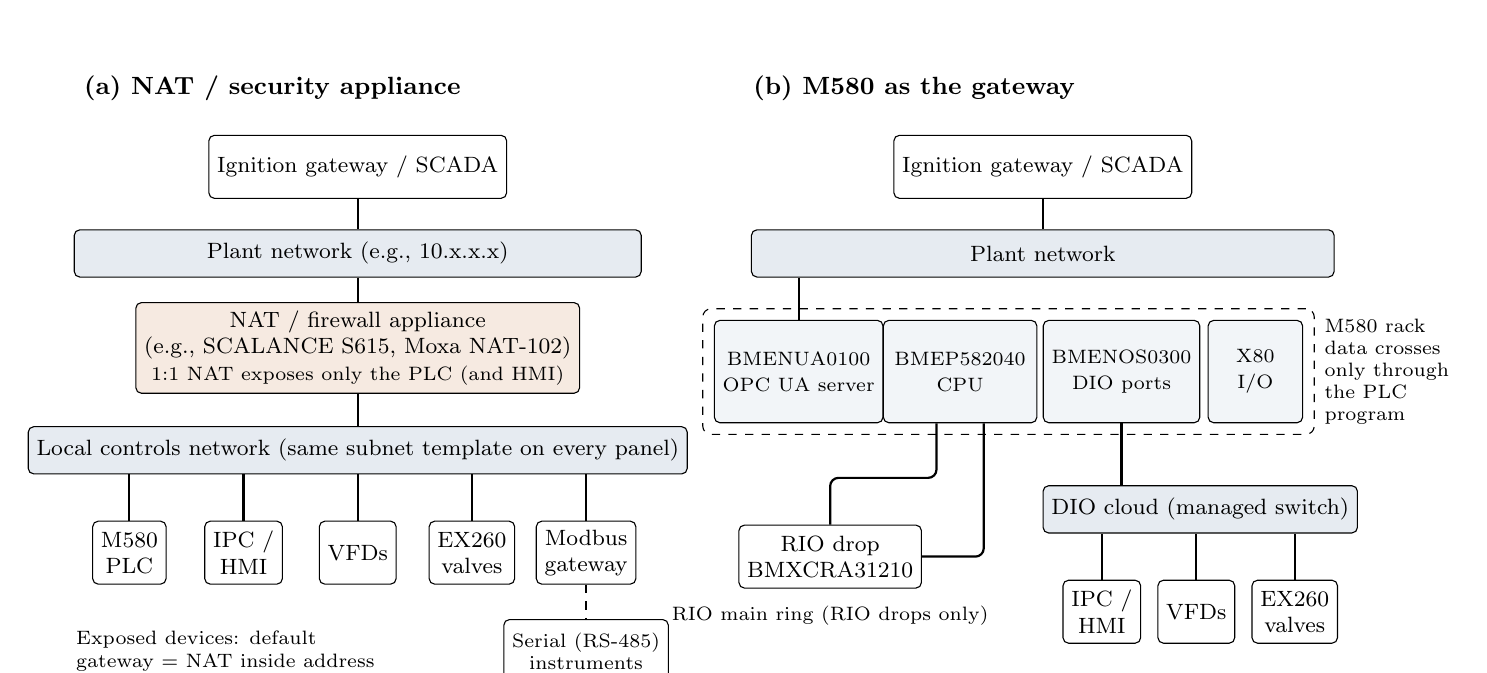
\begin{tikzpicture}[
  font=\footnotesize,
  box/.style={draw, rounded corners=2pt, align=center, minimum height=8mm, inner sep=3pt, fill=white},
  net/.style={draw, fill=headblue!12, rounded corners=2pt, align=center, minimum height=6mm, inner sep=3pt},
  link/.style={-, thick},
  every node/.style={align=center}
]
% ---------- (a) NAT appliance ----------
\node[font=\small\bfseries, anchor=west] at (-7.9,5.9) {(a) NAT / security appliance};
\node[net, minimum width=7.2cm] (plantA) at (-4.3,3.8) {Plant network (e.g., 10.x.x.x)};
\node[box] (scadaA) at (-4.3,4.9) {Ignition gateway / SCADA};
\draw[link] (scadaA) -- (scadaA |- plantA.north);
\node[box, fill=noteorange!12] (nat) at (-4.3,2.6) {NAT / firewall appliance\\(e.g., SCALANCE S615, Moxa NAT-102)\\\scriptsize 1:1 NAT exposes only the PLC (and HMI)};
\draw[link] (plantA) -- (nat);
\node[net, minimum width=7.2cm] (localA) at (-4.3,1.3) {Local controls network (same subnet template on every panel)};
\draw[link] (nat) -- (localA);
\node[box] (plcA) at (-7.2,0.0) {M580\\PLC};
\node[box] (hmiA) at (-5.75,0.0) {IPC /\\HMI};
\node[box] (vfdA) at (-4.3,0.0) {VFDs};
\node[box] (solA) at (-2.85,0.0) {EX260\\valves};
\node[box] (gwA) at (-1.4,0.0) {Modbus\\gateway};
\foreach \n in {plcA,hmiA,vfdA,solA,gwA} \draw[link] (\n.north) -- (\n.north |- localA.south);
\node[box, font=\scriptsize] (serA) at (-1.4,-1.25) {Serial (RS-485)\\instruments};
\draw[link, dashed] (gwA) -- (serA);
\node[font=\scriptsize, align=left, anchor=west] at (-8.0,-1.25) {Exposed devices: default\\gateway = NAT inside address};

% ---------- (b) M580 as gateway ----------
\node[font=\small\bfseries, anchor=west] at (0.6,5.9) {(b) M580 as the gateway};
\node[net, minimum width=7.4cm] (plantB) at (4.4,3.8) {Plant network};
\node[box] (scadaB) at (4.4,4.9) {Ignition gateway / SCADA};
\draw[link] (scadaB) -- (scadaB |- plantB.north);
% M580 rack
\node[box, minimum width=1.95cm, minimum height=1.3cm, fill=headblue!6] (nua) at (1.30,2.3) {\scriptsize BMENUA0100\\\scriptsize OPC UA server};
\node[box, minimum width=1.95cm, minimum height=1.3cm, fill=headblue!6] (cpu) at (3.35,2.3) {\scriptsize BMEP582040\\\scriptsize CPU};
\node[box, minimum width=1.95cm, minimum height=1.3cm, fill=headblue!6] (nos) at (5.40,2.3) {\scriptsize BMENOS0300\\\scriptsize DIO ports};
\node[box, minimum width=1.20cm, minimum height=1.3cm, fill=headblue!6] (io) at (7.10,2.3) {\scriptsize X80\\\scriptsize I/O};
\node[draw, dashed, rounded corners=3pt, inner sep=4pt, fit=(nua)(cpu)(nos)(io), label={[font=\scriptsize, align=left]right:M580 rack\\data crosses\\only through\\the PLC\\program}] (rack) {};
\draw[link] (plantB.south -| nua.north) -- (nua.north);
% RIO main ring from CPU (ring drawn as out-and-back)
\node[box] (rioB) at (1.70,-0.05) {RIO drop\\BMXCRA31210};
\draw[link, rounded corners=3pt] ([xshift=-3mm]cpu.south) -- ([xshift=-3mm]cpu.south |- 0,0.95) -| (rioB.north);
\draw[link, rounded corners=3pt] (rioB.east) -| ([xshift=3mm]cpu.south);
\node[font=\scriptsize] at (1.70,-0.80) {RIO main ring (RIO drops only)};
% DIO cloud from NOS
\node[net, minimum width=3.6cm] (dio) at (6.40,0.55) {DIO cloud (managed switch)};
\draw[link] (nos.south) -- (nos.south |- dio.north);
\node[box] (hmiB) at (5.15,-0.75) {IPC /\\HMI};
\node[box] (vfdB) at (6.35,-0.75) {VFDs};
\node[box] (solB) at (7.60,-0.75) {EX260\\valves};
\foreach \n in {hmiB,vfdB,solB} \draw[link] (\n.north) -- (\n.north |- dio.south);
\end{tikzpicture}}
\caption{Typical panel network layouts. In (a) an appliance translates addresses so only selected devices are visible on the plant network. In (b) the M580 keeps the networks separate: SCADA reads PLC variables through the BMENUA0100 OPC UA server, remote I/O drops are on the RIO main ring, and distributed devices are on a separate DIO cloud connected through a BMENOS0300 (or a dual-ring switch).}
\label{fig:network-layout}
\end{figure}

\subsection{Using the Modicon M580 as a Gateway}\label{sec:m580-gateway}
An M580 can act as the boundary between the plant network and the local controls network without a separate NAT device. The idea is simple: give the PLC separate network connections and let \emph{only the PLC program} pass data between them.
\begin{enumerate}[itemsep=2pt]
  \item \textbf{Local side.} Remote I/O drops go on the RIO main ring from the CPU's ports. Distributed devices (HMI, VFDs, valve banks, gateways) go on a separate DIO cloud, connected through a BMENOS0300 module, a dual-ring switch, or a BMENOC0301/11 --- never directly on the RIO ring. Schneider does not permit RIO modules in a DIO cloud or DIO devices directly on the main ring.\footnote{Schneider Electric, \emph{Modicon M580 Standalone System Planning Guide} (HRB62666) and \emph{System Planning Guide for Complex Topologies} (NHA58892). CPUs ending in ``40'' (e.g., BMEP582040) support RIO; those ending in ``20'' support local and DIO only.}
  \item \textbf{Plant side (standard).} Add a \separt{BMENUA0100} OPC UA module and connect its control port to the plant network. Ignition connects to it as an OPC UA client and browses the PLC variables by name (Section~\ref{sec:protocols}). Configure the module's cybersecurity (it ships with a Secured/Standard mode rotary switch) and confirm in the module configuration that it does not forward traffic between its control port and the device network.
  \item \textbf{Plant side (alternative).} Where Modbus TCP or EtherNet/IP explicit access is needed instead, add a \separt{BMENOC0301} and leave its \emph{Ethernet backplane port disabled} (the default). Schneider's documentation states that the module is then isolated from the rest of the M580 Ethernet network, so the plant network can't see the local devices; the module still exchanges data with the CPU over the X~Bus backplane. Bench test the access to CPU variables in this configuration before relying on it.
  \item \textbf{Give SCADA the data it needs.} SCADA reads and writes only the PLC's own variables. Data from local devices reaches SCADA because the PLC program copies it into those variables.
\end{enumerate}
\textbf{Limitations.} SCADA can't talk directly to a VFD or other local device this way --- everything goes through the PLC. If you need to reach local devices directly (for example to configure a drive from the plant network), use a NAT appliance instead. The \separt{BMENOC0321} control-network module can route traffic between networks (IP forwarding), but that is a routed design, not an isolated one, so it needs the same security review as a NAT appliance. Confirm the exact module configuration in Control Expert for each project.

\textit{Further reading:} \href{https://filedn.eu/l6oFb0aAwOAyRLLaUMiUmzz/CE_HELP/eng/BMENOC03x1/BMENOC03x1_D-SE-0035359.htm}{Schneider Electric --- The BMENOC0301/11 modules in Modicon M580 networks}; \href{https://www.se.com/us/en/product/BMENUA0100/communication-module-modicon-m580-opc-ua/}{Schneider Electric --- BMENUA0100 OPC UA module}.

\section{Communication Protocol Standards}\label{sec:protocols}
\textbf{PLC to SCADA: OPC UA.} Modicon M580 PLCs communicate with the Ignition SCADA server over OPC UA through the \separt{BMENUA0100} module.
\begin{itemize}[itemsep=1pt]
  \item Ignition connects as an OPC UA client and browses the PLC variables by name, so no register maps are needed and each PLC data type maps directly to an Ignition UDT (Section~\ref{sec:udt}).
  \item Expose variables in Control Expert under \textit{Tools \textgreater{} Project Settings \textgreater{} General \textgreater{} PLC embedded data \textgreater{} Data dictionary}. Selecting \textit{Only HMI variables} limits OPC UA access to variables with the HMI attribute set in the data editor; use it so SCADA only sees what it needs.
  \item Use certificate-based security (policy Basic256Sha256, sign and encrypt), named user accounts with the minimum permissions, and the module's Secured mode. Anonymous access is not used.
  \item The M580 CPU itself has only an OPC UA \emph{client} (firmware 4.10 and later); the OPC UA \emph{server} for SCADA is the BMENUA0100.
\end{itemize}

\textbf{Device communications: EtherNet/IP by default, Modbus TCP as the backup.} Communication between the PLC and drives, valve banks, scales, IPCs, and similar devices defaults to \textbf{EtherNet/IP}. \textbf{Modbus TCP} may be used:
\begin{itemize}[itemsep=1pt]
  \item as a backup when a device does not support EtherNet/IP or its EtherNet/IP option is not available (for example the Invertek OPT-3-MTPEG-IN case in Section~\ref{sec:vfd}); or
  \item to convert an existing Modbus RTU (serial) system to Ethernet through a gateway such as the EKI-122x (Section~\ref{sec:protocol-converters}).
\end{itemize}
Modbus addressing and setup are covered in Appendix~\ref{app:modbus}.

\textbf{Exceptions.}
\begin{itemize}[itemsep=1pt]
  \item \textbf{Productivity2000} has no OPC UA server and Ignition has no native Productivity driver, so its SCADA link uses Modbus TCP with a documented register map.
  \item The two existing \textbf{ControlLogix} systems (Rare Gas column and Helium system) use Ignition's Allen-Bradley Logix driver.
\end{itemize}

\section{Addressing}
IP addresses and VLANs must be assigned through the company IP address management process. A project number must not be inserted directly into an octet unless the resulting address and subnet have been allocated. The subnet mask must create the intended boundary; a /16 network must not be treated as though different third octets are isolated. Static addresses, reserved addresses, gateways, VLAN IDs, DNS names, and ownership must be recorded in the network schedule.

Do not use the common vendor default subnets (192.168.0.x and 192.168.1.x) for local controls networks. Many devices and laptops ship on those subnets, and plugging one in causes address conflicts.

\section{Network Equipment}
Managed industrial switches must be used unless the basis of design documents why an unmanaged switch is acceptable. Required features must be selected for the application and may include VLANs, access control, port security, SNMPv3, redundant ring protocol, quality of service, multicast/IGMP management (needed where EtherNet/IP I/O traffic is present), time synchronization, diagnostics, configuration backup, and event logging. Unused switch ports and services must be disabled where supported. Unmanaged switches are never used on an M580 RIO ring.

\section{Remote Access}\label{sec:remote-access}
Direct inbound access to PLCs, HMIs, or panel devices from the internet is prohibited. Remote access must use the company-managed secure access service, MFA, named accounts, authorization, session logging where available, and time-limited vendor access. Permanent vendor modems or cloud tunnels require documented cybersecurity approval.\footnote{CISA, NCSC-UK, FBI, et al., \emph{Secure Connectivity Principles for Operational Technology (OT)}, January 2026; CISA et al., \emph{Guide to Securing Remote Access Software}, June 2023.}

For the parent company's network and remote access platforms, Cato Networks and Claroty xDome Secure Access, see Appendix~\ref{app:cato-claroty}.

\section{System Hardening and Maintenance}\label{sec:hardening}
\note{Nothing is currently done to harden controls systems. A hardening plan should be discussed and adopted.}

The plan should cover:
\begin{itemize}[itemsep=1pt]
  \item An asset list: what is installed, its firmware and software versions, and who owns it.
  \item Changing default passwords on every device.
  \item Turning off unused services (for example FTP, HTTP, and TFTP on PLCs) and unused switch ports.
  \item A practical approach to firmware and Windows updates that weighs security against uptime.
\end{itemize}
Vendor guidance: Schneider Electric, \emph{Modicon Controllers Platform --- Cyber Security Reference Manual} (EIO0000001999); Inductive Automation, \href{https://inductiveautomation.com/resources/article/ignition-security-hardening-guide}{Ignition Security Hardening Guide}.

\textbf{A NAT device is a good first step.}
\begin{itemize}[itemsep=1pt]
  \item \textbf{Hides the local network.} Only the devices you choose (usually the PLC, sometimes the HMI) can be reached from the plant network. VFDs, valve banks, gateways, and everything else stay invisible.
  \item \textbf{Protects devices that can't be hardened.} Many drives, gateways, and older devices can't be patched or locked down. Putting them behind NAT protects them without touching each one --- a ``compensating control'' in ISA/IEC 62443 terms.
  \item \textbf{One place to control access.} With a firewall-capable appliance (Table~\ref{tab:nat-options}), allow-only rules (for example, SCADA server to PLC on the OPC UA port only) and logging live in one box instead of being set on every device.
  \item \textbf{Keeps panels standard.} Every panel can reuse the same local subnet, so panel designs, spares, and vendor setups stay the same from project to project.
\end{itemize}

\section{Time, Logging, and Recovery}
Controllers, SCADA, workstations, network devices, and security systems should use an approved time source and a consistent time zone. Security and operational events must be retained according to company policy. The design must document recovery priorities, replacement configurations, backups, and the test interval for restoring critical OT assets.

\future{set up a plant time server so all controls equipment is synchronized to one source. This will be investigated with IT.}
\begin{itemize}[itemsep=1pt]
  \item \textbf{Why it matters:} alarm and event timestamps, historian data, and the first-out records of trips (Chapter~\ref{ch:plc-standards}) can only be compared across systems if every device uses the same clock.
  \item \textbf{Likely approach:} IT provides an NTP server on the plant network, or the controls network gets its own (for example a GPS-referenced appliance). PLCs, Ignition servers, IPCs, and managed switches sync to it as NTP clients. The M580 CPU can be an NTP client (a BMENOC03x1 can also update the CPU time), and Productivity2000 CPUs sync over SNTP using the Network Time Service instruction.
  \item \textbf{Questions for IT:} which server to use, whether controls networks behind NAT can reach it, and which time zone or UTC convention to standardize on.
\end{itemize}

\chapter{Accounts and Access Control}\label{ch:accounts}
\section{Identity Requirements}
Named individual accounts should be used for normal engineering, administration, and operator access. Shared administrator accounts are limited to controlled emergency (``break-glass'') use or platform constraints. Roles should follow least privilege and separate operator, maintenance, engineering, security administration, and system administration duties where supported.
\note{Individual accounts are not currently implemented. See Section~\ref{sec:ignition-accounts} for the Ignition login discussion.}
\note{It would be good to adopt policies covering:
\begin{itemize}[itemsep=1pt]
  \item Logins and passwords: multi-factor authentication for remote access, storing passwords in a password manager (never in code, drawings, or documents), and changing default passwords.
  \item Shared and emergency accounts: service accounts and ``break-glass'' emergency logins, who owns them, and how they are stored.
  \item Account lifecycle: who approves access, periodic reviews, removing access when people leave, and expiration dates for vendor accounts.
  \item Handing over credentials at turnover, so EFC is not left depending on a contractor's login.
\end{itemize}}

\chapter{PLC Standards}\label{ch:plc-standards}
\section{Program Architecture}
Programs must be organized by equipment or functional area with a documented execution order. Each project must provide a main routine, input processing, equipment modules, sequences, alarm/protective logic, communications, output processing, diagnostics, and HMI interface. Safety-related logic must reside in the approved safety architecture and must be clearly separated from ordinary control logic.

IEC 61131-3 languages may be used according to purpose: ladder diagram for maintainable discrete/equipment logic, function block diagram for continuous control and reusable blocks, and structured text for calculations, data handling, and bounded iteration. Dense or obscure code must be avoided regardless of language.

\section{Naming and Data Quality}
Names must be descriptive, consistent, and traceable to P\&IDs and electrical drawings. Tags exposed outside the controller must include engineering units, range, description, quality/validity, and source where supported. PLC booleans must use \texttt{BOOL}; real process values must use \texttt{REAL} unless precision requirements justify another type. Retentive data must be explicitly identified and minimized.

\section{Operating Modes and Commands}\label{sec:udt-modes}
Equipment modules must distinguish Off, Manual, Auto, Maintenance/Lockout, and Simulation where applicable. HMI requests must not drive physical outputs directly; logic must validate mode, permissives, interlocks, ownership, and command timing. Manual mode must not bypass protective functions. On startup, mode and command restoration must follow the risk assessment and must not create an unexpected start.

\subsection{Mode Definitions (PCLib)}\label{sec:pclib-modes}
\future{These definitions apply to equipment built on the PCLib data types (Appendix~\ref{app:data-types-future}), which are not yet in use on projects. Existing systems keep the Off / Manual / Auto / Lockout pattern of the current types (Appendix~\ref{app:data-types}).}

Every PCLib control module (valve, motor, drive, PID loop, and so on) carries a nested \texttt{T\_Mode} object named \texttt{Mode}. It has exactly four modes. The mode answers one question: \emph{who is allowed to command this device right now?}

\begin{small}
\begin{longtable}{@{}P{2.50cm}P{1.40cm}P{6.40cm}P{6.21cm}@{}}
\caption{PCLib Equipment Modes}\label{tab:pclib-modes} \\
\toprule
\rowcolor{tblhead}\textbf{Mode} & \textbf{HMI} & \textbf{Who commands the device} & \textbf{Typical use} \\
\midrule
\endfirsthead
\multicolumn{4}{@{}l}{\small\textit{Table \thetable{} continued}} \\
\toprule
\rowcolor{tblhead}\textbf{Mode} & \textbf{HMI} & \textbf{Who commands the device} & \textbf{Typical use} \\
\midrule
\endhead
\textbf{Auto} \par{\footnotesize\texttt{Sts\_Mode = 3}} & \textbf{A} & The program: the sequence, phase, or equipment module that owns the device (\texttt{Prog\_} commands). Operator start/stop/open/close commands are ignored. & Normal production under sequence or loop control. \\
\textbf{Manual} \par{\footnotesize\texttt{Sts\_Mode = 2}} & \textbf{M} & The operator, from the SCADA faceplate (\texttt{Cmd\_} commands). Program commands are ignored. & Normal production when the operator runs the device by hand, for example during startup, upsets, or when a sequence is not running. \\
\textbf{Maintenance} \par{\footnotesize\texttt{Sts\_Mode = 1}} & \textbf{MT} & Maintenance or controls personnel, from the SCADA faceplate, using the Maintenance security role. Program commands are ignored and the device cannot be acquired by any sequence. & Testing, stroking, calibrating, or troubleshooting a device while the rest of the system stays in service. \\
\textbf{Out of service} \par{\footnotesize\texttt{Sts\_Mode = 0}} & \textbf{L} & Nobody. Outputs go to their de-energized (safe) state and all commands are ignored. & Device removed, isolated under LOTO, not yet installed, or failed and waiting for repair. \\
\bottomrule
\end{longtable}
\end{small}

\textbf{Rules that apply in every mode.}
\begin{itemize}[itemsep=1pt]
  \item Interlocks (\texttt{Inp\_IntlkOK}) stop running equipment in \emph{every} mode, including Manual and Maintenance. A mode never bypasses an interlock. An interlock may be bypassed only through the timed, authorized bypass of its \texttt{T\_Intlk} group, and only as allowed by the Table of Interlocks and Permissives.
  \item Hardwired E-stops and safety functions are independent of the PLC mode.
  \item Permissives (\texttt{Inp\_PermOK}) block a start in Auto and Manual.
  \item Simulation (\texttt{Sim\_} members) is not a mode. It replaces the field signal and is shown separately on the faceplate.
  \item SCADA requests a mode change; the PLC decides whether to accept it and reports the result in \texttt{Sts\_Mode}. SCADA never assumes the change took effect.
\end{itemize}

\textbf{Manual versus Maintenance.} Both let a person command the device directly, so they are easy to confuse. The difference is \emph{whether the device is still part of the process}:
\begin{longtable}{@{}P{4.20cm}P{6.15cm}P{6.16cm}@{}}
\toprule
\rowcolor{tblhead} & \textbf{Manual (M)} & \textbf{Maintenance (MT)} \\
\midrule
\endhead
Purpose & Running the process by hand & Working \emph{on} the device \\
Who may select it & Operator role & Maintenance role (maintenance technicians, controls engineers) \\
Still available to the process & Yes. A sequence can acquire the device and request Auto (\texttt{Prog\_Auto}). & No. The device cannot be acquired, and any phase or unit that needs it shows it as unavailable and will not start. \\
Permissives & Active & Process permissives that exist only to protect the product or the batch may be marked as bypassable in Maintenance in the Table of Interlocks and Permissives. Equipment and personnel protection permissives stay active. \\
Interlocks & Active & Active \\
Process alarms from the device & Active & May be suppressed by design (ISA-18.2 state G) so operators are not flooded while the device is being worked on. Device fault and equipment-health alarms stay active. \\
Run-time and start counters & Counted & Counted (maintenance runs are still wear) \\
Leaving the mode & To Auto or Maintenance & To Manual only. The operator confirms the device state before returning it to Auto. \\
\bottomrule
\end{longtable}
\note{Whether any permissive may be bypassed in Maintenance, and which process alarms are suppressed, is a design decision made per device, recorded in the Table of Interlocks and Permissives and the alarm list, and reviewed with the PHA. The default is that nothing is bypassed and nothing is suppressed.}

\textbf{Mode changes.} All changes go through Manual, so the device never jumps between Auto and Maintenance or Out of service without a person in control:
\begin{longtable}{@{}P{3.60cm}P{4.80cm}P{8.11cm}@{}}
\toprule
\rowcolor{tblhead}\textbf{Change} & \textbf{Requested by} & \textbf{Conditions} \\
\midrule
\endhead
Manual $\rightarrow$ Auto & Operator (\texttt{Cmd\_Auto}) or owner (\texttt{Prog\_Auto}) & On entering Auto the device follows the owner's current command; owner logic must make that command match the device's state so there is no bump. \\
Auto $\rightarrow$ Manual & Operator (\texttt{Cmd\_Man}) or owner (\texttt{Prog\_Man}) & Blocked while the owner holds a mode lock (\texttt{Prog\_Lock}), for example during a critical phase step. Outputs hold their last state, so the change is bumpless. \\
Manual $\rightarrow$ Maintenance & Maintenance role (\texttt{Cmd\_Maint}) & Only when no sequence owns the device; a supervisor can force a release (\texttt{Cmd\_ForceRelease}). Not available where \texttt{Cfg\_NoMaint} is set. \\
Maintenance $\rightarrow$ Manual & Maintenance role (\texttt{Cmd\_Man}) & Device must be in a known state (for example valve closed, motor stopped). \\
Manual or Maintenance $\rightarrow$ Out of service & Maintenance role (\texttt{Cmd\_OOS}) & Outputs go to the safe state; the device's alarms go out of service (ISA-18.2 state H). \\
Out of service $\rightarrow$ Manual & Maintenance role (\texttt{Cmd\_Man}) & After the device is reinstated and any LOTO is cleared. \\
\bottomrule
\end{longtable}

\textbf{Power-up.} Each device starts in the mode set by \texttt{Cfg\_PowerUpMode}, which defaults to Manual. A device may power up in Auto only where the risk assessment shows it cannot cause an unexpected start. A device left Out of service should stay Out of service after a power cycle; \texttt{T\_Mode} does not do this yet, so it must be added to the library before PCLib is adopted \tbd.

\textbf{SCADA indication.} The faceplate and every equipment symbol show the mode letter (A, M, MT, L) with the same colours on every screen (Appendix~\ref{app:screen-design}). Devices in Maintenance or Out of service are also listed on an overview screen so the shift can see what is not available to the process.

\textbf{Relationship to the current types and to the standards.} Auto, Manual, and Out of service correspond to MTP Automatic, Operator, and Offline; Maintenance is an EFC extension, as ISA-88 defines only Automatic, Semi-automatic, and Manual. The current types' \emph{Lockout} becomes Out of service. The current \emph{Off} is not a mode in PCLib: a stopped device is simply stopped, in Manual or Auto.

\subsection{Setpoint Limits}\label{sec:plc-setpoint-clamp}
Operator-entered values are checked in the PLC, not only in SCADA. For permissive setpoints (Section~\ref{sec:setpoints}) the minimum and maximum are hard-coded in the PLC program; the PLC clamps or rejects any value outside them and reports the active limits to SCADA for display. The limits are changed only through a software revision, under MOC where Section~\ref{sec:review-release} applies.

\section{Data Types (UDTs)}\label{sec:udt}
A user-defined type (UDT) is a reusable data structure that bundles everything about one piece of equipment or one signal --- commands, status, setpoints, alarms, and diagnostics --- into a single variable. Modicon Control Expert calls these \textbf{DDTs} (Derived Data Types); UDT is the general term used by Ignition and most other platforms.

\textbf{Why we use them:}
\begin{itemize}[itemsep=1pt]
  \item Every pump, valve, or analog input of the same kind has the same members with the same names, on every project.
  \item They pair with reusable function blocks (Section~\ref{sec:reusable-fbs}): the block holds the logic, the DDT holds the data.
  \item Programming, SCADA screens, and troubleshooting are faster because the structure is familiar.
\end{itemize}

\textbf{Rules of thumb:}
\begin{itemize}[itemsep=1pt]
  \item Name types with the \texttt{DDT\_} prefix (for example \texttt{DDT\_Valve}) and use one consistent capitalization style for member names.
  \item Use the standard type library shared across projects; do not create project-specific copies of a standard type.
  \item Changing a type changes every instance of it. Treat changes to standard types like any other controlled change (Section~\ref{sec:source-control}), and test them (Section~\ref{sec:change-testing}).
  \item Analog scaling must handle divide-by-zero, invalid configuration, underrange, overrange, and bad quality. Alarm comparison must use the scaled value only when quality is acceptable, unless a separate instrument-fault alarm is intended.
  \item Equipment types keep request, command, status, permissive, interlock, feedback, fault, warning, and runtime data as separate members.
\end{itemize}
The current data types, with their members, are listed in Appendix~\ref{app:data-types}. The proposed replacement library (PCLib), aligned with ISA-88, ISA-18.2, and ISA-101, is described in Appendix~\ref{app:data-types-future}; it is not yet in use on projects.

\subsection{Using UDTs Between the PLC and SCADA}
\begin{itemize}[itemsep=2pt]
  \item \textbf{One type on each side.} Each PLC data type has a matching Ignition UDT with the same member names and structure. A PLC instance (for example \texttt{P101} of type \texttt{DDT\_Motor\_VFD}) is brought into Ignition as one UDT instance, so faceplates and templates are built once per type and reused for every instance.
  \item \textbf{OPC UA.} With the M580 standard (Section~\ref{sec:protocols}), Ignition browses the PLC variables and their DDT structure directly through the BMENUA0100. Only variables marked with the HMI attribute in Control Expert are exposed, so mark the instances SCADA needs and leave internal working variables unmarked.
  \item \textbf{Read versus write.} SCADA writes only to request/command members (for example \texttt{HMI\_Auto}, \texttt{HMI\_CMD}) and operator setpoints. Status, interlock, and feedback members are read-only from SCADA. This matches the rule that HMI requests never drive outputs directly (Section~\ref{sec:udt-modes}).
  \item \textbf{Keep both sides in sync.} When a PLC type changes, the matching Ignition UDT is updated in the same revision and both are tested together.
  \item \textbf{Productivity2000.} Communication uses Modbus TCP, so each structure is mapped to consecutive registers and a register map is required (Appendix~\ref{app:modbus}).
\end{itemize}

\section{Interlocks and First-Out}
Interlock logic must use a structured condition type rather than parallel unstructured arrays. Each condition must include enable, raw condition, active, latched, bypassed, first-out, message/identifier, and timestamp where supported. The summary must include any-active, trip-active, reset-permitted, bypass-present, and first-out index. The number of conditions must be sized by the reusable library and not silently truncated.

Interlocks must fail to the defined state on bad or stale inputs when required by the risk assessment. Reset must not clear an active initiating condition. Bypasses must survive or clear on restart only as defined by the approved bypass policy.

\section{Sequences}
Sequences must use an explicit state model with named steps, entry actions, continuous actions, exit conditions, timeout, hold, abort, restart, and recovery behavior. The sequence structure must include active state, previous state, transition reason, elapsed time, timeout, permissive summary, faulted/held/complete status, and operator requests. Restart after download or power loss must be deterministic and risk assessed.

\section{Communications and Diagnostics}
Communications must include heartbeat or sequence checking where suitable, timeout, data-valid status, stale-data handling, and documented fail behavior. Raw received data must be separated from validated values used by control. Diagnostic status must be available to SCADA without flooding operators with non-actionable alarms.

\section{Reusable Function Blocks}\label{sec:reusable-fbs}
\subsection{What a Function Block Is}
A reusable function block is a block of PLC logic written once and used for every pump, valve, analog input, or sequence of the same kind, so each one behaves the same way. In Control Expert these are \textbf{DFBs} (Derived Function Blocks). The current DFBs are documented in Appendix~\ref{app:function-blocks}.

\subsection{The Standard Object: DFB, DDT, and Ignition UDT}
Each standard equipment type is a matched set of three parts:
\begin{itemize}[itemsep=1pt]
  \item a \textbf{DFB} that holds the logic (for example \texttt{DFB\_Valve});
  \item a \textbf{DDT} that holds the data (for example \texttt{DDT\_Valve}, Section~\ref{sec:udt}); and
  \item an \textbf{Ignition UDT} with its faceplate and templates that present it on SCADA.
\end{itemize}
The three are designed, versioned, and changed together. A change to one is checked against the other two.

\subsection{When to Make One}
Make a DFB for logic that is used more than once or that represents a standard equipment type. One-off logic stays in the project program, where it is easier to read in place.

\subsection{Design Rules}
\begin{itemize}[itemsep=1pt]
  \item Pass the equipment's DDT to the block as an input/output parameter, so the block reads and writes one structure.
  \item No direct I/O addresses or global variables inside the block; everything comes through its pins.
  \item Choose fail-safe default values for every input and parameter.
  \item Start each block with a header comment giving its purpose, revision, author, and date.
  \item Use the standard Off / Manual / Auto / Lockout mode pattern (Section~\ref{sec:udt-modes}).
  \item Keep protective logic visible: interlocks and E-stop inputs come in through pins (for example \texttt{Interlock} and \texttt{Estop} on \texttt{DFB\_Valve}) so they can be seen and traced at the call, not buried inside the block.
\end{itemize}

\subsection{Library Management}
Standard DFBs are kept in a master library (the Control Expert type library). Projects use copies; project-specific changes never overwrite the master. A DFB's revision follows the revision approach in Section~\ref{sec:source-control}. Changing a DFB that contains interlock or protective logic requires an MOC (Section~\ref{sec:review-release}) and a Change Test Record (Appendix~\ref{app:change-test}).
\note{Formal library versioning is not current practice. Git (Appendix~\ref{app:git}) is the planned way to track library changes in the future.}

\subsection{Testing}
New or changed blocks are tested in the simulator before they are used, covering every mode, the interlock and E-stop inputs, and bad-quality inputs. The test is kept on file with the library.

\subsection{Productivity2000}
Productivity Suite does not use DFBs. Reusable logic is built with User Defined Instructions (UDIs, Productivity Suite v4.5 and later), which can be stored in a UDI library (v4.7 and later). The same rules apply: one UDI per equipment type, used with a matching data structure.

\section{Common Systems}
Common systems should use a consistent control structure, naming convention, HMI faceplate, alarm approach, and test procedure. Project-specific limits and options may vary, but the basic operator experience and PLC interface should remain recognizable from project to project.

\subsection{PDC Compressor}\label{sec:pdc-compressor}
The PDC compressor module should organize the package interface into operating mode, start/stop requests, permissives, active interlocks, running status, load state, process values, warnings, trips, first-out indication, and maintenance counters.

The control narrative and code should address, as applicable, suction and discharge pressure, stage temperatures, cooling-water flow and temperature, hydraulic or oil-system status, diaphragm or process-gas leak detection, purge/vent status, valve position, motor feedback, vendor-panel communications, minimum stop time, and restart following a trip or power loss. Setpoints and shutdown actions must come from approved PDC documentation, the process design, and the project hazard review rather than from generic defaults.

The proposed PCLib type for this package is \texttt{T\_DiaComp} (Appendix~\ref{app:data-types-future}, Section~\ref{sec:pclib-t-diacomp}) \newmark. It holds one nested motor for the shared crankshaft, stage 1 and stage 2 pressures, temperatures and head oil pressures, crankcase oil, cooling water, leak detection per stage, purge, diaphragm run-hour counters, and a first-out trip code.
\future{\texttt{T\_DiaComp} replaces the current project-specific compressor type once it has been reviewed against the PDC documentation, the FBD logic, and the existing UDT.}

\chapter{SCADA and HMI Standards}\label{ch:scada}
\section{Ignition Architecture}
Ignition is the preferred SCADA/HMI platform for new projects. The differences between a standard Ignition gateway and Ignition Edge Panel, and how the two are integrated, are covered in Appendix~\ref{app:edge-panel}. The project team should choose the Gateway, database, client, and redundancy arrangement based on system size, availability needs, performance, and recovery time. Operator workstations should normally run Perspective or Vision clients rather than host the production Gateway or database.

Record the tag providers, projects, databases, historian, alarm pipelines, identity provider, certificates, modules, backups, and important external dependencies. Use a development or test environment when practical instead of making untested changes directly in production.

\subsection[Version and Upgrades]{Version and Upgrades \newmark}\label{sec:ignition-version}
EFC runs Ignition~8.1 (Table~\ref{tab:software-versions}). New projects are built on the version the site's Gateway runs; a project is not built on a newer version than the Gateway that will host it. Modules that are not part of the standard Ignition install (third-party drivers, Sepasoft, and similar) need EFC approval because they add licence, support, and upgrade dependencies.
\future{An upgrade to Ignition~8.3 is planned. 8.3 keeps Gateway configuration as files on disk and adds a REST API, which changes how backups and source control work (Appendix~\ref{app:git}). Projects started before the upgrade should avoid features that do not carry over cleanly; the upgrade plan will list them.}

\section{Project and Tag Design}
Use shared projects, inheritance, UDTs, templates, and common scripts to avoid duplicating the same work across projects. Tag names and folders should follow the PLC equipment model and use consistent units, ranges, descriptions, quality handling, alarms, and history settings.

Keep scripts readable and reusable. Log errors that will help with troubleshooting, but avoid repetitive logging that hides useful information. Where a tag, expression, binding, or shared function can do the job cleanly, prefer it over copying scripts into many components.

\section[PLC Connections]{PLC Connections \newmark}\label{sec:ignition-plc-connections}
\begin{itemize}[itemsep=1pt]
  \item \textbf{One device connection per PLC}, named after the PLC (for example the project number and PLC name used in the file name, Section~\ref{sec:source-control}). Connection settings and the security mode are recorded in the system documentation.
  \item \textbf{Protocols} follow Section~\ref{sec:protocols}: OPC UA to M580 PLCs through the BMENUA0100, Modbus TCP to Productivity2000, and the Logix driver to the existing ControlLogix systems.
  \item \textbf{UDTs match PLC data types} member for member, so a PLC instance maps to one Ignition UDT instance with one parameter for its path (Section~\ref{sec:udt}).
  \item \textbf{Scan rates} (tag groups) are chosen for what the data is used for. Use a normal rate (typically 1~s) for most tags, a slower rate for maintenance counters and configuration, and a faster rate only where an operator or a calculation needs it. Leased or driven tag groups can reduce load for tags that are only shown on some screens.
  \item \textbf{Writes} from Ignition go only to command, setpoint, and configuration members (\texttt{Cmd\_}, \texttt{Prm\_}, \texttt{Cfg\_} and the current-type equivalents). Status and input members are read-only in the UDT. The PLC checks and clamps every written value (Section~\ref{sec:plc-setpoint-clamp}).
  \item \textbf{Bad quality} is shown on the screen, never hidden behind the last good value.
\end{itemize}

\section{HMI Philosophy}
Screens should make the current process condition easy to understand. Use color mainly to show abnormal conditions or items requiring attention. Do not rely on color alone; use text, symbols, and state indication as well. Navigation, faceplates, trends, units, decimal precision, manual controls, and alarm presentation should work the same way throughout the project.

Use a clear display hierarchy, normally including overview, area, unit, equipment-detail, and diagnostic screens. Operators should be able to see the active mode, command ownership, equipment state, alarms, interlocks, and bypasses before issuing a command. Use confirmation prompts for consequential actions without adding unnecessary prompts to routine work.

\section{Perspective Design}
Perspective screens follow the Perspective Screen Design Standard in Appendix~\ref{app:screen-design}. Perspective views should be tested at the screen sizes and aspect ratios expected in service. Use responsive containers where resizing is required. Docked views, popups, embedded views, parameters, and message handlers should have clear interfaces and should not depend on fragile component paths.

Startup and navigation scripts should be safe to run more than once, finish quickly, and handle missing tags or bad-quality data without breaking the view. Reusable views should not assume that every optional parameter is present.

\section{Alarms}
Configure Ignition alarms from the approved alarm list. Include the identifier, priority, message, cause, consequence, expected response, deadband, delay, shelving permissions, and any state-based suppression. Acknowledging an alarm does not clear the process condition that caused it.

\textbf{Annunciation and acknowledgment.} Ignition annunciates alarms. For PLC data types that carry their own alarm state (the PCLib types, Appendix~\ref{app:data-types-future}), acknowledging the alarm in Ignition writes through to the alarm's \texttt{Cmd\_Ack} member in the PLC, so the PLC and SCADA states stay the same. Alarms are not acknowledged separately in two places. \newmark

\textbf{Priority.} Alarm priority uses Ignition's built-in priority levels. PLC data types that carry a priority use the same numbers, so a priority set in the PLC carries straight into Ignition without a lookup table: \newmark

\begin{small}
\begin{longtable}{@{}P{1.40cm}P{3.20cm}P{12.33cm}@{}}
\caption{Alarm Priority Numbering}\label{tab:alarm-priority} \\
\toprule
\rowcolor{tblhead}\textbf{Value} & \textbf{Ignition priority} & \textbf{Use} \\
\midrule
\endfirsthead
\toprule
\rowcolor{tblhead}\textbf{Value} & \textbf{Ignition priority} & \textbf{Use} \\
\midrule
\endhead
0 & Diagnostic & Equipment and system diagnostics for maintenance; not shown on the operator alarm summary by default. \\
1 & Low & Operator response needed, with time to respond and a minor consequence. \\
2 & Medium & Prompt response needed to avoid an upset or equipment damage. \\
3 & High & Immediate response needed to avoid a trip, release, or major equipment damage. \\
4 & Critical & Reserved for the most severe consequences; use sparingly. \\
\bottomrule
\end{longtable}
\end{small}
\note{PCLib v1.00 (Appendix~\ref{app:data-types-future}) still numbers \texttt{Cfg\_Priority} 1=Emergency to 4=Low. The generator will be changed to the numbering above at the next PCLib revision.}
Priority is assigned during alarm rationalization from the consequence and the time available to respond (Section~\ref{sec:alarm-mgmt} and Appendix~\ref{app:alarm-doc}), not chosen per tag by the programmer.

Test alarm journals and notification pipelines, including loss and recovery of the database or notification service. Review nuisance, chattering, standing, and frequently occurring alarms after startup.

\section{Historian and Data}
Historize data that has a defined operating, quality, maintenance, regulatory, or analysis purpose. Choose the sampling mode, deadband, timestamp source, and retention period to match that purpose. Document store-and-forward behavior and how bad or uncertain quality is handled.

Database connections should use managed credentials and only the permissions they need. Use encrypted connections when supported by the approved architecture.

\section{Security and Audit}
\subsection*{Individual accounts}\label{sec:ignition-accounts}
Every operator, engineer, and other user should have their own Ignition account and be logged in before using the system. Individual logins mean that actions such as setpoint changes, alarm acknowledgments, and bypasses are recorded against a person, and that each user gets only the access their role needs.
\note{Not currently implemented. This should be discussed in the near future, including how logins work on shared operator stations --- for example automatic logout after inactivity and a fast way to switch users at the station.}
\future{Ignition Perspective can use single sign-on (SSO) through an identity provider using OpenID Connect 1.0 or SAML 2.0, such as Microsoft Entra ID (Azure AD) or Okta. Users would log in with their existing company account rather than a separate Ignition password, and accounts would be added or removed centrally when people join or leave. This works for Perspective, Vision, the Designer, and the Gateway in both 8.1 and 8.3, and is worth looking into, possibly with the parent company's IT group.}

\subsection*{Roles and audit}
Use the approved identity provider when practical and assign access by role. Typical roles include operator, maintenance, engineering, supervisor, and administrator. Audit important actions such as setpoint changes, alarm shelving, recipe changes, and security administration.

OPC UA connections should use trusted certificates, a supported security policy (Basic256Sha256, sign and encrypt), named accounts with the minimum permissions needed, and no anonymous access (Section~\ref{sec:protocols}). Remove default accounts and unused connections before turnover.

\section{Backup, Deployment, and Recovery}
Create a Gateway backup before and after significant production changes and after commissioning. Record the Ignition version, installed modules, licenses, database dependencies, certificates, identity-provider settings, DNS/NTP needs, and restore steps.

For critical systems, demonstrate that the backup can be restored and that the project can be rolled back if a deployment fails. Keep the accepted backup with the project turnover package.

\chapter{Reference Material}
\section{Standards Referenced}\label{sec:standards-referenced}
The project basis of design must identify the editions adopted by the jurisdiction and the editions contractually required. The table below lists each standard cited in this guide once, with the edition cited and where it is used. When a new edition is published, this is the one place to check what needs updating. Applicability must be determined per project.

\begin{longtable}{@{}P{6.05cm}P{10.88cm}@{}}
\caption{Standards Referenced}\label{tab:references}\\
\toprule \rowcolor{tblhead}\textbf{Standard (edition cited)} & \textbf{Subject and where used in this guide}\\ \midrule
\endfirsthead
\multicolumn{2}{@{}l}{\small\textit{Table \thetable{} continued}} \\
\toprule \rowcolor{tblhead}\textbf{Standard (edition cited)} & \textbf{Subject and where used in this guide}\\ \midrule
\endhead
\multicolumn{2}{@{}l}{\textit{Electrical and machinery}} \\
\href{https://link.nfpa.org/all-publications/70/2023}{NFPA 70 (NEC), 2023} & National Electrical Code. Art.~250 grounding and bonding (Section~\ref{sec:bonding}); 409.22 SCCR (Section~\ref{sec:sccr}); 450.3(B) transformer protection (Appendix~\ref{app:transformer-sizing}); Art.~501 Class I locations (Appendix~\ref{app:c1d2}). The 2026 edition is published; confirm the edition adopted by the jurisdiction. \\
NFPA 70E, company-adopted edition & Electrical safe work practices and risk controls. \\
\href{https://link.nfpa.org/all-publications/79/2024}{NFPA 79, 2024} & Electrical equipment of industrial machinery: stop categories and E-stop (Section~\ref{sec:estop}), technical documentation (Appendix~\ref{app:drawing-package}), testing and verification (Appendix~\ref{app:sample-fat}, Section~\ref{sec:change-testing}). \\
\href{https://www.shopulstandards.com/ProductDetail.aspx?productId=UL508A}{UL 508A, 3rd ed. (2018), revised through 2025} & Industrial control panels: construction, markings, and SCCR (Supplement SB). \\
\href{https://webstore.iec.ch/en/publication/26037}{IEC 60204-1:2016+A1:2021} & Electrical equipment of machines: stop categories, pushbutton and indicator colors (Section~\ref{sec:estop}), verification and retesting. \\
ISO 13850:2015 & Emergency stop function (Section~\ref{sec:estop}). \\
\href{https://www.iso.org/standard/73481.html}{ISO 13849-1:2023} & Safety-related parts of machinery control systems. \\
\href{https://webstore.iec.ch/en/publication/59927}{IEC 62061:2021} & Functional safety of machinery safety-related control systems. \\
\multicolumn{2}{@{}l}{\textit{Hazardous locations}} \\
NFPA 496, 2024 & Purged and pressurized enclosures (Appendix~\ref{app:c1d2}). \\
UL 121201, 9th ed. & Nonincendive equipment for Class I and II, Division 2 locations (Appendix~\ref{app:c1d2}). \\
UL 698A, 4th ed. (2018, reaffirmed 2022) & Industrial control panels relating to hazardous locations (intrinsically safe circuits). \\
\multicolumn{2}{@{}l}{\textit{Documentation}} \\
IEC 61082-1:2014 & Preparation of documents used in electrotechnology (Appendix~\ref{app:drawing-package}). \\
IEC 81346-1:2022 and 81346-2:2019 & Reference designations (Appendix~\ref{app:drawing-package}). \\
IEEE 315-1975 (inactive-reserved) / IEC 60617 & Graphic symbols for electrical diagrams. \\
ISA-5.1, adopted edition & Instrumentation symbols and identification. \\
\multicolumn{2}{@{}l}{\textit{Process safety, alarms, and testing}} \\
OSHA 29 CFR 1910.119 & Process safety management: (i) pre-startup safety review, (l) management of change (Sections~\ref{sec:online-changes} and~\ref{sec:change-testing}). \\
IEC 61511-1:2016+A1:2017 / ANSI/ISA-84 & Functional safety for safety instrumented systems; bypass and modification rules. \\
\href{https://www.isa.org/products/ansi-isa-18-2-2016-management-of-alarm-systems-for}{ANSI/ISA-18.2-2016} and IEC 62682:2022 & Alarm management lifecycle (Section~\ref{sec:alarm-mgmt} and Appendix~\ref{app:alarm-doc}). \\
\href{https://www.isa.org/products/isa-101-01-2015-human-machine-interfaces-for}{ANSI/ISA-101.01-2015} & HMI philosophy, design, implementation, operation, and maintenance. \\
IEC 62381:2024 (Ed.~3) & Factory, site, and site integration acceptance tests (Appendix~\ref{app:sample-fat}). \\
ISA-TR18.2.7-2017 & Alarm management for packaged systems (Section~\ref{sec:packaged-equipment}). \\
ISA-88 series, where applicable & Batch-control models, terminology, and modular structure. \\
\multicolumn{2}{@{}l}{\textit{Cybersecurity}} \\
IEC 62443-2-4:2023 (Ed.~2) & Security program requirements for IACS service providers (integrators and maintenance contractors) (Section~\ref{sec:contractor-cyber}). \\
\href{https://www.isa.org/standards-and-publications/isa-standards/isa-iec-62443-series-of-standards}{ISA/IEC 62443-2-1:2024, 62443-3-2:2020, 62443-3-3:2013} & Security program (configuration management, logging), zones and conduits, and system security requirements (Chapter~\ref{ch:networking}, Section~\ref{sec:online-changes}). \\
\href{https://csrc.nist.gov/pubs/sp/800/82/r3/final}{NIST SP 800-82 Rev.~3 (2023)} & OT cybersecurity guidance. A later revision must not replace Rev.~3 in project requirements until issued as final and adopted by EFC. \\
CISA et al., \emph{Secure Connectivity Principles for OT} (2026) & Remote and external connectivity to OT (Section~\ref{sec:remote-access}). \\
\bottomrule
\end{longtable}

Manufacturer manuals, certificates, and application notes must be retained for the actual product revision used. A web link is informational and does not replace a controlled project copy of required technical data.

\section[EFC Internal References]{EFC Internal References \newmark}\label{sec:internal-refs}
\begin{small}
\begin{longtable}{@{}P{5.20cm}P{11.73cm}@{}}
\caption{EFC Internal References}\label{tab:internal-refs} \\
\toprule
\rowcolor{tblhead}\textbf{Item} & \textbf{What it is and where it is kept} \\
\midrule
\endfirsthead
\multicolumn{2}{@{}l}{\small\textit{Table \thetable{} continued}} \\
\toprule
\rowcolor{tblhead}\textbf{Item} & \textbf{What it is and where it is kept} \\
\midrule
\endhead
This standard (LaTeX source) & Source for this document and its appendix PDFs. Rebuild the PDFs from the source; do not edit the PDFs. Each released revision is tagged in Git (\texttt{rev-G}, \texttt{rev-H}, \ldots). \\
Separate appendix PDFs & One PDF per appendix, built with the main document, for handing to contractors (Section~\ref{sec:efc-provides}). \\
PCLib (EFC Repo, \texttt{PCLib/}) & Proposed standard data types: the generator \texttt{gen\_pclib.py}, the Control Expert and Ignition import files, the member list, and the source of Appendix~\ref{app:data-types-future}. \\
Current data types and DFBs & The DDTs and DFBs in Appendices~\ref{app:data-types} and~\ref{app:function-blocks}, kept in the Control Expert master library (Section~\ref{sec:udt}). \\
Standard hardware selections & Chapter~\ref{ch:hardware}, with prices and ordering history kept in the hardware pricing archive. \\
Perspective Screen Design Standard & Appendix~\ref{app:screen-design} and its fluid text style sheet. \\
\bottomrule
\end{longtable}
\end{small}
\note{A formal location for the EFC Repo (company Git server or hosted service) and who may change it have not been decided.}

\section[Manufacturer Documentation]{Manufacturer Documentation \newmark}\label{sec:mfr-docs}
The manuals below are the ones most often needed for EFC systems. Download the revision that matches the hardware firmware and software version in use and keep a copy with the project, as required above.

\begin{small}
\begin{longtable}{@{}P{6.60cm}P{2.80cm}P{7.53cm}@{}}
\caption{Key Manufacturer Documents}\label{tab:mfr-docs} \\
\toprule
\rowcolor{tblhead}\textbf{Document} & \textbf{Number} & \textbf{Use} \\
\midrule
\endfirsthead
\multicolumn{3}{@{}l}{\small\textit{Table \thetable{} continued}} \\
\toprule
\rowcolor{tblhead}\textbf{Document} & \textbf{Number} & \textbf{Use} \\
\midrule
\endhead
\multicolumn{3}{@{}l}{\textit{Schneider Electric --- Modicon M580 and Control Expert}} \\
\href{https://www.se.com/us/en/download/document/EIO0000001578/}{Modicon M580 Hardware Reference Manual} & EIO0000001578 & CPU, rack, power supply, and module hardware. \\
\href{https://www.se.com/us/en/download/document/998-21389419_GMA-US/}{Designing Successful Modicon M580 Architectures} (white paper) & 998-21389419 & Choosing local, remote, and distributed I/O architectures (Chapter~\ref{ch:networking}). \\
\href{https://www.se.com/us/en/download/document/HRB62666}{M580 Standalone: Frequently Used Architectures} & HRB62666 & Reference network layouts for single-CPU systems. \\
\href{https://www.se.com/us/en/download/document/EIO0000001590/}{M580 Change Configuration on the Fly} & EIO0000001590 & Adding modules and I/O to a running system (Section~\ref{sec:online-changes}). \\
Modicon Controllers Cybersecurity User Guide & EIO0000001999 & Hardening M580 PLCs and Control Expert (Section~\ref{sec:protocols} and Chapter~\ref{ch:networking}). \\
\href{https://www.se.com/us/en/faqs/FAQ000208173/}{BMENUA0100 forbidden architectures} (FAQ) & FAQ000208173 & Check before finalizing the OPC UA module's network connections. \\
\multicolumn{3}{@{}l}{\textit{Inductive Automation --- Ignition}} \\
\href{https://docs.inductiveautomation.com/docs/8.1/intro}{Ignition 8.1 User Manual} & --- & Gateway, tags, alarms, Perspective (Chapter~\ref{ch:scada}). \\
Ignition Security Hardening Guide & --- & Gateway security settings (Chapter~\ref{ch:networking}). \\
\multicolumn{3}{@{}l}{\textit{AutomationDirect --- Productivity2000}} \\
Productivity Suite help file and P2000 hardware user manual & P2-USER-M & Programming, Modbus mapping, and hardware for the low-cost PLC option. \\
\bottomrule
\end{longtable}
\end{small}

\section[Further Reading]{Further Reading \newmark}\label{sec:further-reading}
\subsection*{Free papers}
\begin{itemize}[itemsep=1pt]
  \item B.~Hollifield, \emph{Understanding and Applying the ANSI/ISA-18.2 Alarm Management Standard} (PAS, 2010). Written for the 2009 edition, but still a clear summary of the alarm lifecycle and rationalization.
  \item ISA, \emph{Industrial Cybersecurity for Small- and Medium-Sized Businesses} (updated 2024). A practical starting point for an OT security program.
  \item ISAGCA, \emph{Quick Start Guide: An Overview of the ISA/IEC 62443 Standards} (2024). Which parts of the series apply to an asset owner, an integrator, and a product supplier.
  \item ISAGCA, \emph{Leveraging ISA 62443-3-2 for IACS Risk Assessment} (2021). The zones, conduits, and risk assessment workflow.
\end{itemize}

\subsection*{ISA technical reports for sections still being developed}
These are paid documents. ISA members can read them on ISA Pub Hub.
\begin{small}
\begin{longtable}{@{}P{7.20cm}P{9.73cm}@{}}
\toprule
\rowcolor{tblhead}\textbf{Document} & \textbf{Where it would help} \\
\midrule
\endhead
ISA-TR101.01-2022, HMI Philosophy, and ISA-TR101.02-2019, HMI Usability and Performance & HMI Philosophy (Chapter~\ref{ch:scada}) and the screen design standard. \\
ISA-TR18.2.1-2018, Alarm Philosophy; ISA-TR18.2.3, Basic Alarm Design & A site alarm philosophy and the alarm settings in the data types (Appendix~\ref{app:alarm-doc}). \\
ISA-TR18.2.7-2017, Alarm Management When Utilizing Packaged Systems & Alarms from vendor packages (Section~\ref{sec:packaged-equipment}). \\
ISA-TR88.00.02-2022, Machine and Unit States & Equipment state models in the data types. \\
ANSI/ISA-106.00.01-2023 and related technical reports & Procedural automation for startup and shutdown sequences. \\
\bottomrule
\end{longtable}
\end{small}

\subsection*{Training}
\begin{itemize}[itemsep=1pt]
  \item \href{https://inductiveuniversity.com/}{Inductive University}: free Ignition training and the Ignition Core certification.
  \item Schneider Electric training: Control Expert and M580 courses through the local distributor or Schneider's training centers.
  \item Inductive Automation Forum and the Schneider Community \emph{Industrial Automation How-to} board: the most useful places to search for practical M580-to-Ignition questions.
\end{itemize}

\appendix
\chapter{Perspective Screen and Template Scaling Procedure}
\label{app:perspective-scaling}
\setlength{\emergencystretch}{3em}

\textbf{Applies to:} Ignition Perspective 8.1 process views designed at 1000 $\times$ 800, deployed on 1920 $\times$ 1080 and 3840 $\times$ 2160 operator displays. Recheck the procedure during migration to 8.3. The view size, physical monitor resolution, and session viewport are three different measurements.

\section{Purpose and design basis}
Create one maintainable set of process screens and reusable equipment views. Use the actual 1000 $\times$ 800 view canvas as the coordinate reference. The target monitors are 16:9; the design canvas is 5:4. Uniformly scaling a 5:4 canvas into 16:9 space leaves unused space, unless the screen is redesigned, cropped, or stretched. Windows scaling, browser zoom, Workstation mode, taskbars, and docked views also change the usable viewport. Record those settings for each workstation class before selecting font sizes or evaluating fit.

The process diagram shall preserve geometry. Operator text and controls shall remain legible and usable at the smallest deployed viewport. Physical 4K resolution alone does not require larger CSS font sizes; at 200\% operating-system scaling, the available CSS viewport may resemble a 1080p display.

\section{Set up the page and process view}
\begin{enumerate}[leftmargin=*,itemsep=3pt]
\item Identify the deployed screen modes: display resolution, OS scaling, browser or Perspective Workstation, browser zoom, fullscreen/window mode, and dock dimensions. Measure the actual viewport available to the primary view.
\item Create the representative process view with a default size of 1000 $\times$ 800. Set its root Coordinate Container \texttt{props.mode} to \texttt{percent}. If the complete diagram must preserve its original 5:4 geometry, set \texttt{props.aspectRatio} to \texttt{5:4}. Do not set \texttt{16:9} merely because the monitor is 16:9. If the process content has a different intended ratio, measure that content area separately.
\item Keep navigation, alarms, and supporting panels in separate Flex containers or docked views. Decide how to use spare space around a 5:4 diagram on a 16:9 monitor. If filling all available width is required, redesign the layout for that width rather than distorting the symbols and pipes.
\item Add equipment as Embedded View instances. Place the instances with relative positions in the parent Coordinate Container. For a design coordinate $(x,y,w,h)$ in the 1000 $\times$ 800 reference, use $(x/1000,y/800,w/1000,h/800)$. For example, a valve at $(250,200)$ with a 24 $\times$ 24 footprint uses $(0.25,0.25,0.024,0.03)$.
\item Keep a consistent process-layer order for background, pipes, equipment, indicators, and interactive overlays. Check that resized overlays still line up with their symbols.
\end{enumerate}

\section{Build reusable equipment templates}
Each valve, motor, pump, compressor, and process-value display shall be its own parameterized view. The template default size is a \emph{design footprint}, not the SVG's intrinsic resolution. For a dense 1000 $\times$ 800 P\&ID, begin with compact symbols and short callouts. The values below are trial dimensions on that design canvas; actual content and operator interaction determine the final sizes.

\begin{center}
\begin{tabular}{@{}p{5.05cm}p{3.73cm}p{6.86cm}@{}}
\toprule
Template & Starting footprint & Contents / sizing check\\ \midrule
Valve symbol & 24 $\times$ 24 px & Separate interactive hit region if needed\\
Motor symbol & 28 $\times$ 28 px & State on symbol; name nearby\\
Pump symbol & 32 $\times$ 28 px & State on symbol; name nearby\\
Compressor symbol & 40 $\times$ 32 px & State on symbol; details in faceplate\\
Valve with short callout & 60 $\times$ 36 px & Brief tag or state only\\
Process value callout & 104 $\times$ 42 px & Short tag; value and units\\
\bottomrule
\end{tabular}
\end{center}

\begin{enumerate}[leftmargin=*,itemsep=3pt]
\item Use a compact symbol view when only the SVG and state are needed. Use a separate short callout or a symbol-plus-callout view when the tag and value must travel with it. Long messages and command details belong in an equipment faceplate or popup. A Percent Coordinate Container suits spatial symbol assemblies; a Flex Container suits flowing text.
\item Give each SVG a correct \texttt{viewBox} and preserve its intrinsic aspect ratio. In an Image component use a containing fit, not a fill mode that distorts the symbol. If individual SVG parts must change color from bindings, use an appropriate embedded SVG/Drawing strategy and validate it in the installed 8.1 minor version.
\item Use view parameters for equipment identity, tag paths, name, units, and optional state. Bind SVG color, status text, and process values within the template. Include explicit bad-quality and communication-loss states.
\item Size the parent Embedded View instance to the intended footprint. Inspect the Embedded View's width and height default settings. Start with both set to \texttt{false} for a resizable instance, then verify no scrollbars, clipping, or unexpected internal sizing. These settings are not a universal text-scaling switch.
\item Keep commands, status messages, and numeric values as Perspective components when they must be interactive or data-bound. A separate text component can scale independently of its adjacent SVG; its style must be tested explicitly.
\end{enumerate}

\section{Text, interaction, and state rules}
The Percent Coordinate Container scales component bounds and locations, but a label's CSS font size needs its own rule. Keep SVG geometry and interactive text as distinct components within each template. Apply named Style Classes to the actual Label components; inspect components that expose separate internal text-style properties.

\subsection{Define text roles}
Use the existing text roles for full-size callouts, faceplates, and details. For compact P\&ID callouts, start with \texttt{compactName}, \texttt{compactValue}, and \texttt{compactUnits} in the companion CSS file. Their base sizes are 12, 16, and 12 CSS px respectively. Do not place full status sentences inside a small symbol. These are trial values, not Ignition requirements or a substitute for operator review.

\begin{center}
\begin{tabular}{@{}p{4.91cm}p{3.62cm}p{7.11cm}@{}}
\toprule
Style Class & Base font size & Use\\ \midrule
\texttt{equipmentName} & 16 px & Equipment tag and short name, e.g., P-101\\
\texttt{processValue} & 20--24 px bold & Primary numeric reading\\
\texttt{processUnits} & 14--16 px & psig, $^\circ$C, GPM\\
\texttt{equipmentStatus} & 16--18 px bold & RUNNING, FAULT, LOCAL\\
\texttt{interactionMessage} & 16--18 px & Disabled command or interlock message\\
\bottomrule
\end{tabular}
\end{center}

\subsection{Use the fluid text stylesheet}
For Ignition 8.1.22 or later, use the accompanying \texttt{Perspective-Fluid-Text-Styles.css} in the project's Advanced Stylesheet. In the Designer, expand Perspective \(\rightarrow\) Styles. If \texttt{stylesheet.css} does not exist, right-click Styles and select \emph{Enable Advanced Stylesheet}. Open \texttt{stylesheet.css}, paste the supplied CSS rules, and save the project. This file is a paste-ready stylesheet, not a standalone one-click Style Class import.

On each Label, enter the unprefixed name in \texttt{props.style.classes}. For a compact value use \texttt{compactValue}; a separate units Label uses \texttt{compactUnits}. The full-size roles listed above are for larger displays. Perspective adds the \texttt{.psc-} prefix to CSS selectors. Enter the class name on the component without this prefix or a leading dot. Do not set a competing inline \texttt{fontSize}.

The CSS uses \texttt{clamp(minimum, fluid size, maximum)}. For example, \texttt{clamp(16px, 1.4815vmin, 32px)} produces roughly 16 px at a 1920 $\times$ 1080 CSS viewport and 32 px at 3840 $\times$ 2160. It changes continuously between those \emph{viewport} sizes. \texttt{vmin} does not measure the 1000 $\times$ 800 view or an individual Embedded View. If the diagram retains a fixed 1000 $\times$ 800 rendered size while the viewport grows, these font rules can outgrow the callouts. In that case, keep compact fonts fixed or base sizing on the rendered view container after validating browser support. At 200\% OS scaling, a 3840-pixel display may expose a viewport near 1920 CSS pixels. Docks, browser chrome, and zoom also affect the result. Check both workstations.

If the installed 8.1 minor version predates the Advanced Stylesheet feature, enter the corresponding \texttt{clamp()} value directly as the Label's \texttt{props.style.fontSize} or use ordinary Style Classes after confirming the expression renders correctly in that version. Keep those values centralized when the project is upgraded.

\subsection{Provide room for labels and interactions}
Enlarging the font does not enlarge its allocated label box automatically. Reserve space for the longest equipment identifier, negative sign, precision, units, and worst-case status. Keep number and units in separate components if their sizes differ. Use a Flex Container for a symbol with flowing text, or increase the template and label footprints at larger layouts. For long messages, define a two-line wrap area or show a short state on the diagram with detail in a faceplate or popup. Do not shrink text until arbitrary messages fit or let it overlap neighboring equipment.

Keep an interactive target large enough to select reliably; 44 $\times$ 44 CSS px is a starting trial for touch operation, subject to site HMI requirements and operator review. A 24 px visual symbol can have a larger transparent hit region, but adjacent hit regions must not overlap. Show abnormal state with text or symbols as well as color. Keep confirmation, permissive, interlock, and command feedback visible and unambiguous.

\subsection{Worked example: process value template}
Create a compact instance of \texttt{Templates/Process Value} around 104 $\times$ 42 on the 1000 $\times$ 800 canvas. Put a short tag on the first line and the reading plus units on the second, using \texttt{compactName}, \texttt{compactValue}, and \texttt{compactUnits}. Represent bad quality with an unmistakable short indicator and show the full message in the faceplate. Test the longest actual tag, \texttt{-9999.99 psig}, and a bad-quality state. If they do not fit, widen the callout or abbreviate the tag consistently; do not hide or truncate critical values. Place several instances in the representative process screen and check both workstation configurations, including the right dock.

\section{Verification and acceptance}
\begin{enumerate}[leftmargin=*,itemsep=3pt]
\item Build one representative view containing at least one of each template type, the longest expected equipment name and message, a bad-quality value, an alarmed item, and a command target.
\item Open the session on actual 1920 $\times$ 1080 and 3840 $\times$ 2160 stations with their deployed OS scaling, zoom, docks, and Workstation/browser mode. Record the effective viewport dimensions.
\item Confirm symbols and pipes retain alignment and shape; no view has unwanted scrollbars, clipping, overlap, or stretched SVGs. Inspect labels, units, number precision, quality indication, and long messages.
\item Confirm every interactive target can be selected reliably and that popups and commands remain visible. Check normal, running, stopped, fault, alarm, disabled, and communication-loss conditions relevant to each template.
\item Repeat the test after upgrading to 8.3, including representative SVG color bindings, embedded view sizing, style classes, and interaction behavior. Record any changes before releasing the upgraded project.
\end{enumerate}

\section{Maintenance rule}
Keep this appendix source in the Controls Standard LaTeX project. When changing the screen or template sizing guidance, update this file, the standalone procedure PDF, and the compiled Controls Standard PDF in the same revision. Record the affected Ignition version and recheck the two deployed screen configurations.

\section*{Ignition documentation}
\begin{itemize}[leftmargin=*]
\item \href{https://www.docs.inductiveautomation.com/docs/8.1/appendix/components/perspective-components/perspective-container-palette/perspective-coordinate-container}{Perspective Coordinate Container (8.1)}
\item \href{https://www.docs.inductiveautomation.com/docs/8.1/ignition-modules/perspective/views-in-perspective/embedded-views}{Embedded Views (8.1)}
\item \href{https://www.docs.inductiveautomation.com/docs/8.1/ignition-modules/perspective/styles/style-classes}{Style Classes (8.1)}
\item \href{https://www.docs.inductiveautomation.com/docs/8.1/ignition-modules/perspective/working-with-perspective-components/images-and-icons-in-perspective}{Images and Icons in Perspective (8.1)}
\end{itemize}

\chapter{Important Equations and Calculations}
\label{app:equations}

This appendix collects the main design calculations referenced in Chapter~\ref{ch:hardware}. Each one is written as a short, step-by-step method with a worked example, and every equation links to a source that explains it in more detail.

\section{Short-Circuit Current Rating (SCCR)}
\label{app:eq-sccr}
\textbf{Used in:} Section~\ref{sec:sccr}. The panel's SCCR must be equal to or greater than the available fault current where the panel is installed.

\textbf{How to work it out (simple version).} UL 508A Supplement SB uses a ``weakest link'' approach: the panel is only as strong as its lowest-rated power component.
\begin{enumerate}[itemsep=2pt]
  \item \textbf{Get the available fault current} at the panel location. This comes from the facility's electrical engineer, a short-circuit study, or the utility. Write it down; it goes on the drawings.
  \item \textbf{List every component in the power circuit} --- main disconnect, fuses and breakers, power distribution blocks, motor starters and overloads, contactors, VFDs, and the primary side of control transformers. Control-circuit parts on the secondary of a control transformer usually do not count.
  \item \textbf{Write down each component's SCCR} from its nameplate, datasheet, or the manufacturer's tested-combination table. If a part has no rating, UL 508A assigns it a low default value (often 5~kA), which usually ends up being the weak link.
  \item \textbf{Take the lowest number.} That is the panel SCCR:
\end{enumerate}
\[
  \text{SCCR}_{\text{panel}} = \min\left(\text{SCCR}_{1},\ \text{SCCR}_{2},\ \dots,\ \text{SCCR}_{n}\right) \;\geq\; I_{\text{available fault}}
\]
\begin{enumerate}[resume,itemsep=2pt]
  \item \textbf{Compare it to the available fault current.} If the panel SCCR is too low, replace the weak component with a higher-rated one or use a manufacturer's tested combination (for example a specific fuse class protecting a VFD or a motor starter).
\end{enumerate}
UL 508A also lets you raise some component ratings when they are protected by current-limiting fuses or breakers. That is an advanced step --- ask before relying on it.

\textbf{Example.} The facility says 22~kA is available at the panel.
\begin{center}
\small
\begin{tabular}{@{}P{12.52cm}R{4.80cm}@{}}
\toprule
Component & SCCR \\ \midrule
Main fused disconnect (Class J fuses) & 100 kA \\
Power distribution block (stand-alone rating) & 10 kA \\
Motor starter (manufacturer combination rating) & 65 kA \\
VFD (with the fuses listed in its manual) & 65 kA \\
Control transformer primary fuse holder (Class CC) & 200 kA \\ \midrule
\textbf{Lowest value = panel SCCR} & \textbf{10 kA} \\
\bottomrule
\end{tabular}
\end{center}
10~kA is less than 22~kA, so the panel fails. Swapping the distribution block for one rated 100~kA when protected by Class J fuses makes the lowest value 65~kA, and $65 \geq 22$, so the panel passes and is marked ``SCCR: 65~kA.''

\textit{Further reading:} \href{https://www.eaton.com/us/en-us/products/electrical-circuit-protection/short-circuit-current-ratings.html}{Eaton --- Short-Circuit Current Ratings (SCCR) resource page}; \href{https://www.eaton.com/content/dam/eaton/products/electrical-circuit-protection/fuses/solution-center/bus-ele-tech-lib-short-circuit-current-rating-calculations-and-marking-2008-spd.pdf}{Bussmann --- SCCR calculations and marking (UL 508A SB)}; \href{https://www.mersen.com/sites/default/files/files_imported_ep/TT-SCN1-Achieving-Higher-Short-Circuit-Current-Ratings-for-Industrial-Control-Panels-Tech-Topic.pdf}{Mersen --- Achieving higher SCCR for industrial control panels}.

\section{Enclosure Heat and Cooling}
\label{app:eq-heat}
\textbf{Used in:} Section~\ref{sec:heat}. Check the heat at the hottest expected ambient temperature.

\subsection*{Step 1 --- Add up the heat inside the panel}
Add the heat loss (in watts) of every device. Use the ``power loss'' or ``heat dissipation'' value from each datasheet. Typical sources:
\begin{itemize}[itemsep=1pt]
  \item \textbf{Power supplies:} not all input power reaches the output. Heat $= P_{\text{out}}\left(\dfrac{1}{\eta} - 1\right)$, where $\eta$ is efficiency. A 240~W supply at 92\% efficiency gives off about 21~W.
  \item \textbf{VFDs:} roughly 2--3\% of the drive's rated power, or use the datasheet value.
  \item \textbf{PLC racks, I/O, switches, PCs:} use the datasheet watts (power drawn is roughly heat given off).
  \item \textbf{Relays, contactor coils, transformers:} a few watts each; transformers list their losses.
\end{itemize}
\[
  P_{\text{heat}} = \sum P_{\text{device}} \quad [\text{W}]
\]

\subsection*{Step 2 --- Work out how much heat the enclosure can shed on its own}
A closed steel enclosure loses heat through its outside walls. How much it can lose depends on its exposed surface area and how much hotter you let the inside get compared to the room:
\[
  P_{\text{natural}} = k \times A \times \Delta T
\]
\begin{itemize}[itemsep=1pt]
  \item $k \approx 5.5~\text{W}/(\text{m}^2\cdot\text{\textdegree C})$ for painted steel (about $0.28~\text{W}/(\text{ft}^2\cdot\text{\textdegree F})$).
  \item $A$ = exposed surface area. Don't count a side that is mounted against a wall or another enclosure.
  \item $\Delta T$ = maximum inside temperature you allow minus the maximum ambient temperature.
\end{itemize}

\subsection*{Step 3 --- Compare, and pick a cooling method}
If $P_{\text{heat}} \leq P_{\text{natural}}$, natural cooling is enough. If not, add cooling:
\[
  \text{Fan airflow (CFM)} = \frac{3.17 \times P_{\text{heat}}~[\text{W}]}{\Delta T~[\text{\textdegree F}]}
  \qquad\qquad
  \text{AC size (BTU/hr)} = 3.412 \times P_{\text{total}}~[\text{W}]
\]
For an air conditioner, $P_{\text{total}}$ is the internal heat \emph{plus} the heat soaking in through the walls when the room is hotter than the panel ($k \times A \times (T_{\text{ambient}} - T_{\text{inside}})$). Add about 20--30\% margin to fan airflow for filter and airflow-path losses.

\begin{center}
\small
\begin{tabular}{@{}P{8.66cm}P{8.66cm}@{}}
\toprule
\rowcolor{tblhead}\textbf{Situation} & \textbf{Use} \\ \midrule
Heat load is below what the enclosure sheds on its own & \textbf{Natural cooling.} Sealed enclosure, no fan. \\
Too much heat, but room air is clean, dry, and at least \textasciitilde5~\textdegree C (10~\textdegree F) cooler than the allowed inside temperature & \textbf{Filtered fan} (fan in, filtered vent out). Cheapest active option; filters need regular cleaning. \\
Room air is dirty, wet, oily, or corrosive, or the panel must stay NEMA 4/4X/12, but the room is still cooler than the allowed inside temperature & \textbf{Air-to-air heat exchanger} (keeps the enclosure sealed). \\
Room is as hot or hotter than the allowed inside temperature, or the heat load is large & \textbf{Air conditioner.} Also the usual choice for outdoor panels in direct sun. \\
Hazardous (classified) location & Cooling equipment must be rated for the area (see Section~\ref{sec:c1d2}). \\
\bottomrule
\end{tabular}
\end{center}

\textbf{Example.} A wall-mounted 36" H $\times$ 30" W $\times$ 12" D steel enclosure. Room maximum is 30~\textdegree C and we want the inside to stay at or below 40~\textdegree C, so $\Delta T = 10$~\textdegree C (18~\textdegree F).
\begin{itemize}[itemsep=1pt]
  \item Exposed area (front, top, bottom, two sides; back is on the wall) $= 1080 + 720 + 864 = 2664~\text{in}^2 \approx 1.72~\text{m}^2$.
  \item Natural capacity: $5.5 \times 1.72 \times 10 \approx 95$~W.
  \item Heat load: 24~V power supply 21~W + PLC rack 40~W + industrial PC 25~W + network switch 10~W + two small VFDs 80~W $= 176$~W.
  \item $176 > 95$, so natural cooling is not enough. The air is clean, so use a fan: $3.17 \times 176 / 18 \approx 31$~CFM; with 30\% margin, choose a filtered fan of at least \textbf{40~CFM}.
  \item If the room could reach 45~\textdegree C instead, a fan can't cool below room temperature, so use an air conditioner: wall heat gain $= 5.5 \times 1.72 \times 5 \approx 47$~W, total $= 223$~W, and $3.412 \times 223 \approx 760$~BTU/hr. Choose the next standard size up (e.g., \textbf{1,000~BTU/hr}).
\end{itemize}

\textit{Further reading:} \href{https://www.nvent.com/sites/default/files/acquiadam/assets/Heat\%20dissipation_En_nVent_HOFFMAN_2.pdf}{nVent HOFFMAN --- Calculating heat dissipation in enclosures (white paper)}; \href{https://www.proventofan.com/how-to-calculate-electrical-enclosure-cooling-formula-example-and-fan-sizing/}{Electrical enclosure cooling --- fan airflow formula and example}.

\section{Control Transformer Sizing}
\label{app:transformer-sizing}
\textbf{Applies to:} control power transformers (CPTs) that take plant power (for example 480~VAC) and make 120~VAC for panel control circuits --- power supplies, the PLC, contactor coils, fans, lights, and a service receptacle.

\subsection{The Short Version}
\begin{enumerate}[itemsep=2pt]
  \item Decide how the transformer connects (primary and secondary voltage).
  \item Add up the \textbf{sealed (steady) VA} of everything on 120~VAC.
  \item Add 25\% and round up to the next standard size.
  \item Check that the transformer can handle the \textbf{inrush} when coils pull in.
  \item Size the primary and secondary fuses.
  \item Pick a part and wire it per the nameplate.
\end{enumerate}

\subsection{Step-by-Step}
\subsubsection*{Step 1 --- Decide how it connects}
A 480~VAC \emph{delta} system has three hot lines and no neutral. A single-phase control transformer is connected \textbf{line-to-line} across two of the phases (for example L1 and L2), so its primary sees 480~V. The secondary is 120~V. One side of the secondary (X2) is bonded to ground to make the grounded (neutral) conductor; the other side (X1) is the fused hot.

Most control transformers have dual-voltage windings (for example 240$\times$480 primary, 120$\times$240 secondary). You set the voltage with jumpers shown on the nameplate.

\subsubsection*{Step 2 --- Add up the sealed VA}
``Sealed'' VA is what each device draws once it is running. Get it from the datasheet; for power supplies use input VA (output power $\div$ efficiency $\div$ power factor), not output watts. Only count loads that can be on at the same time.
\[
  \text{VA}_{\text{sealed}} = \sum \text{VA}_{\text{each device}}
\]

\subsubsection*{Step 3 --- Add margin and round up}
Add 25\% for growth and continuous loading, then pick the next standard size up. Common sizes are 50, 75, 100, 150, 250, 350, 500, 750, 1000, 1500, 2000, 3000, and 5000~VA.
\[
  \text{VA}_{\text{required}} = 1.25 \times \text{VA}_{\text{sealed}}
\]

\subsubsection*{Step 4 --- Check inrush}
When a contactor or relay coil first pulls in, it draws several times its sealed VA for a few cycles. If many coils pull in at once, the transformer's output voltage dips; if it dips too far, coils chatter or don't close. Combine the sealed load with the inrush of the coils that can energize at the same moment:
\[
  \text{VA}_{\text{inrush selection}} = \sqrt{\left(\text{VA}_{\text{sealed}}\right)^2 + \left(\text{VA}_{\text{inrush}}\right)^2}
\]
Then look up the chosen transformer in the manufacturer's \emph{regulation} (inrush) chart, usually in the 90\% secondary voltage column at 40\% power factor. The transformer's listed inrush rating must be at least your calculated value. If not, go up one size.

\subsubsection*{Step 5 --- Size the fuses}
The National Electrical Code (NEC 450.3(B), and 430.72(C) for motor control circuits) sets the maximum fuse size. For a transformer with \emph{both} primary and secondary fuses:
\begin{center}
\small
\begin{tabular}{@{}P{5.95cm}P{4.54cm}P{6.38cm}@{}}
\toprule
\rowcolor{tblhead}\textbf{Where} & \textbf{Rated current} & \textbf{Maximum fuse size} \\ \midrule
Primary & any (with secondary fuse) & 250\% of primary current \\
Secondary & 9 A or more & 125\% (next standard size allowed) \\
Secondary & less than 9 A & 167\% \\
Primary only (no secondary fuse) & 9 A or more & 125\% \\
Primary only (no secondary fuse) & 2 A to 9 A & 167\% \\
Primary only (no secondary fuse) & less than 2 A & 300\% (500\% allowed by 430.72(C) for control circuits) \\
\bottomrule
\end{tabular}
\end{center}
\[
  I_{\text{primary}} = \frac{\text{VA}}{V_{\text{primary}}}
  \qquad\qquad
  I_{\text{secondary}} = \frac{\text{VA}}{V_{\text{secondary}}}
\]
Use \textbf{time-delay} fuses (for example Class CC time-delay) on the primary so the transformer's own magnetizing inrush doesn't blow them. Both primary lines are fused because neither leg of a 480~V delta is grounded. On the secondary, fuse only X1; X2 is the grounded conductor.

\subsection{Worked Example: 480~VAC Delta to 120~VAC}
A panel is fed from a 3-phase, 480~VAC delta supply and needs 120~VAC control power. The 120~VAC loads are (example values --- use your actual datasheets):
\begin{center}
\small
\begin{tabular}{@{}P{10.81cm}R{3.03cm}R{3.03cm}@{}}
\toprule
\rowcolor{tblhead}\textbf{Load} & \textbf{Sealed VA} & \textbf{Inrush VA} \\ \midrule
24~VDC power supply, 240~W output (92\% efficient, PF 0.95) & 275 & --- \\
Modicon BMXCPS3500 PLC power supply & 75 & --- \\
Enclosure fan & 40 & --- \\
LED panel light & 15 & --- \\
Service receptacle (NEC counts 180~VA) & 180 & --- \\
Three contactor coils (10~VA sealed / 100~VA inrush each) & 30 & 300 \\ \midrule
\textbf{Total} & \textbf{615} & \textbf{300} \\
\bottomrule
\end{tabular}
\end{center}

\begin{enumerate}[itemsep=4pt]
  \item \textbf{Connection.} Single-phase transformer, primary across L1--L2 at 480~V, secondary 120~V with X2 bonded to ground.
  \item \textbf{Sealed VA} $= 615$~VA.
  \item \textbf{Margin:} $1.25 \times 615 = 769$~VA $\Rightarrow$ next standard size is \textbf{1000~VA}.
  \item \textbf{Inrush check} (all three contactors pulling in together):
  \[
    \sqrt{615^2 + 300^2} = \sqrt{378{,}225 + 90{,}000} \approx 684~\text{VA}
  \]
  Look up the 1000~VA model in the manufacturer's regulation chart (90\% column). Its inrush rating must be at least 684~VA; 1000~VA control transformers are normally rated well above that, so 1000~VA is fine. Confirm on the chart for the exact part.
  \item \textbf{Fuses.}
  \begin{itemize}[itemsep=1pt]
    \item Primary current: $1000 / 480 = 2.08$~A. Maximum with secondary protection: $2.5 \times 2.08 = 5.2$~A $\Rightarrow$ \textbf{5~A time-delay Class CC}, one in each primary line (2 fuses).
    \item Secondary current: $1000 / 120 = 8.33$~A. Less than 9~A, so the maximum is $1.67 \times 8.33 = 13.9$~A $\Rightarrow$ \textbf{10~A} fuse on X1 (leaves margin above the 8.33~A rating).
  \end{itemize}
  \item \textbf{Select a part.} For example, the \href{https://www.lamonde.com/ph1000mqmj.html}{Hammond Power Solutions PH1000MQMJ}: 1000~VA, 240$\times$480~V primary, 120$\times$240~V secondary. Jumper the primary for 480~V and the secondary for 120~V exactly as shown on its nameplate diagram. Add finger-safe fuse blocks for the primary and secondary fuses, or choose the factory fuse-kit version (PH1000MQMJ-FK) if available.
\end{enumerate}

\textbf{Result:} 1000~VA, 480~V to 120~V control transformer; 2 $\times$ 5~A time-delay primary fuses; 1 $\times$ 10~A secondary fuse on X1; X2 bonded to ground.

\subsection{Further Reading}
\begin{itemize}[itemsep=2pt]
  \item \href{https://www.elliottelectric.com/StaticPages/ElectricalReferences/Guides/control-transformer-selection-guide.aspx}{Elliott Electric --- Control transformer selection guide (inrush VA equation and regulation chart)}
  \item \href{https://literature.rockwellautomation.com/idc/groups/literature/documents/wp/1497-wp001_-en-p.pdf}{Rockwell Automation --- Proper selection of control circuit transformers (white paper)}
  \item \href{https://electrical-engineering-portal.com/overcurrent-protection-transformer-nec-450-3}{Electrical Engineering Portal --- Overcurrent protection of transformers (NEC 450.3)}
\end{itemize}

\chapter{Modbus Addressing on the M580 and Productivity2000}
\label{app:modbus}

This appendix explains how Modbus works, how to set up Modbus addressing on our two PLC platforms --- the Modicon M580 (Control Expert Classic) and the AutomationDirect Productivity2000 (Productivity Suite) --- and how to match those addresses in Ignition. Software versions are listed in Section~\ref{sec:software-versions}.

\textbf{When Modbus is used:} EFC's standards are OPC UA between the M580 and SCADA and EtherNet/IP for device communications (Section~\ref{sec:protocols}). Modbus is used for the backup and conversion cases: a device without EtherNet/IP, an EtherNet/IP option that is not available, an existing Modbus RTU system being converted to Ethernet, and Productivity2000 SCADA links (which have no OPC UA server).

\textbf{Scope:} Modbus TCP, Modbus RTU where a device requires it, and Modbus/TCP Security.

\section{Modbus Basics}
Modbus is a request/response protocol: a client asks and a server answers. Servers never send data on their own, so every value SCADA shows was polled. All data lives in four tables.

\begin{longtable}{@{}P{3.25cm}P{2.18cm}P{2.39cm}P{2.18cm}P{1.74cm}P{3.91cm}@{}}
\toprule
\textbf{Table} & \textbf{Size} & \textbf{Access} & \textbf{Legacy prefix} & \textbf{Read FC} & \textbf{Write FC} \\
\midrule
\endhead
Coils & 1 bit & Read/write & 0xxxx & 01 & 05 single, 15 multiple \\
Discrete inputs & 1 bit & Read-only & 1xxxx & 02 & --- \\
Input registers & 16-bit word & Read-only & 3xxxx & 04 & --- \\
Holding registers & 16-bit word & Read/write & 4xxxx & 03 & 06 single, 16 multiple \\
\bottomrule
\end{longtable}

\subsection*{Function codes in common use}
\begin{longtable}{@{}P{1.88cm}P{9.40cm}P{5.63cm}@{}}
\toprule
\textbf{FC} & \textbf{Name} & \textbf{Per-request limit} \\
\midrule
\endhead
01 / 02 & Read coils / discrete inputs & 2000 bits \\
03 / 04 & Read holding / input registers & 125 registers \\
05 / 06 & Write single coil / register & 1 \\
15 & Write multiple coils & 1968 bits \\
16 & Write multiple registers & 123 registers \\
22 & Mask write register (set bits inside a word) & 1 \\
23 & Read/write multiple registers in one transaction & 125 read / 121 write \\
43/14 & Read device identification & --- \\
\bottomrule
\end{longtable}

\subsection*{Framing}
\begin{itemize}[itemsep=2pt]
  \item \textbf{Modbus RTU (serial):} binary frames on RS-485/RS-232 with a slave address (1--247) and CRC. One master per bus.
  \item \textbf{Modbus TCP:} the same message with a 7-byte header (transaction ID, protocol ID, length, unit ID) on TCP port 502. No CRC.
  \item \textbf{RTU over TCP:} raw RTU frames (with CRC) over a TCP socket, common on low-cost serial-to-Ethernet converters. Not the same as Modbus TCP; the client driver must match.
  \item \textbf{Unit ID:} ignored by most native TCP devices (use 255 or 1). Through a gateway it selects the serial slave address.
\end{itemize}

\subsection*{Exception codes}
\begin{longtable}{@{}P{1.41cm}P{5.40cm}P{10.10cm}@{}}
\toprule
\textbf{Code} & \textbf{Name} & \textbf{Usual cause} \\
\midrule
\endhead
01 & Illegal function & Device does not support that FC (for example FC16 or FC22) \\
02 & Illegal data address & Off-by-one, or a request spanning an undefined address \\
03 & Illegal data value & Value out of range, or quantity above the device limit \\
04 & Server device failure & Internal device fault \\
06 & Server busy & Long command in progress; retry \\
0A / 0B & Gateway path / target failed & Gateway cannot reach the serial device: unit ID, wiring, baud \\
\bottomrule
\end{longtable}

\section{Addressing and Data Types}
Most Modbus problems are an off-by-one address or a swapped word order. Settle both in writing for every device before building tags.

\subsection*{Address notation}
The protocol itself only carries a 0-based offset (0--65535) within a table. Documentation adds other numbering on top:
\begin{longtable}{@{}P{5.87cm}P{3.52cm}P{7.51cm}@{}}
\toprule
\textbf{Notation} & \textbf{First holding register} & \textbf{Where it is used} \\
\midrule
\endhead
Offset (0-based) & 0 & Wire captures, Modicon \%MW numbers, Ignition with zero-based on \\
Register number (1-based) & 1 & Most device manuals, Ignition default \\
Legacy 5-digit & 40001 & Older manuals; the leading 4 names the table \\
Extended 6-digit & 400001 & Devices with more than 9999 registers; Productivity Suite \\
\bottomrule
\end{longtable}
40001, 400001, 1-based HR1, and \%MW0 all point to the same register (offset 0). The conversion is:
\[
  \text{offset} = \text{register number} - 1 = \text{legacy address} - 40001 = \text{6-digit address} - 400001
\]
Confirm any vendor map by reading a known value before building the full tag set (\href{https://www.modbus.org/modbus-specifications}{Modbus Application Protocol Specification}).

\subsection*{Data types and word order}
\begin{itemize}[itemsep=2pt]
  \item Modbus only defines bits and 16-bit words. INT/UINT use one register; DINT, UDINT, and REAL use two; LREAL and LINT use four; strings use one register per two characters.
  \item Bytes within a register are big-endian. The order of the two words in a 32-bit value is not standardized: high word first (ABCD) or low word first (CDAB).
  \item \textbf{The Modicon M580 stores 32-bit values low word first} in consecutive \%MW. Ignition must have \emph{Reverse Word Order} on for these devices.
  \item Test with known values: 123.456 in a REAL and 70000 in a DINT. A word swap shows up as an obviously wrong number.
\end{itemize}

\section{Platform Comparison}
\begin{longtable}{@{}P{3.90cm}P{6.50cm}P{6.50cm}@{}}
\toprule
& \textbf{Modicon M580 (Control Expert Classic)} & \textbf{Productivity2000 (Productivity Suite)} \\
\midrule
\endhead
Where Modbus addresses come from & You assign them: located variables at fixed \%MW / \%M addresses & Assigned per tag in the Tag Database (MOD Start column), automatically or by hand \\
Address numbering & \%MW\textit{n} = offset \textit{n} (0-based) & 6-digit, 1-based (e.g., 400001) as shown in the Tag Database \\
32-bit word order & Low word first & Confirm with a test value (see Section~\ref{app:modbus:p2000}) \\
Modbus TCP server & Built into the CPU, port 502 & Built into the CPU, port 502; enable on the Ethernet port \\
Modbus RTU & Through an X80 serial module (BMXNOM0200) or a gateway & Built-in serial ports \\
PLC as Modbus client & I/O scanning (DTM Browser) or READ\_VAR / WRITE\_VAR & MRX (read) and MWX (write) instructions \\
Ignition settings & Zero-based on, Reverse Word Order on & Zero-based off (1-based); set word order to match the test value \\
\bottomrule
\end{longtable}

\section{Step-by-Step: Modicon M580 in Control Expert Classic}
\label{app:modbus:m580}
The M580 is a Modbus TCP server on port 502 and can also act as a client. Only \textbf{located} variables (\%M, \%MW) can be read over Modbus; unlocated variables and DDT instances cannot. These steps are written for Control Expert Classic v16.2.

\subsection*{Setting up the M580 as a Modbus server}
\begin{enumerate}[itemsep=2pt]
  \item \textbf{Size the located memory.} In the Project Browser, open the CPU in the PLC bus configuration and go to its \emph{Configuration} tab. Set the number of \%M bits and \%MW words large enough for the full SCADA map plus room to grow (see the register map layout in Section~\ref{app:modbus:rules}).
  \item \textbf{Declare located variables.} In the Data Editor, create each variable SCADA needs and enter its address in the \emph{Address} column, for example \texttt{PT101\_PV} (REAL) at \texttt{\%MW200}. Put REAL, DINT, and UDINT values on even addresses and never locate anything on the second word of a 32-bit value.
  \item \textbf{Copy between your DDTs and the map.} DDT instances (DDT\_Process\_Value, DDT\_Device, and so on) can't be read over Modbus directly. In a dedicated section of the program, copy status values from the DDTs into the located map each scan, and copy commands and setpoints from the map back into the DDTs after checking limits.
  \item \textbf{Lock down access.} On the CPU's \emph{Security} tab, enable the access control list and list only the Ignition servers and engineering stations allowed to connect. Enforce Security disables FTP, TFTP, HTTP, EtherNet/IP, SNMP, and DHCP/BOOTP; re-enable only what the project needs.
  \item \textbf{Test.} Write known test values into a REAL and a DINT, then read them with a standalone Modbus client (Modbus Poll, QModMaster) before setting up Ignition.
  \item \textbf{Ignition device settings.} Port 502, Zero-based Addressing \textbf{on}, Reverse Word Order \textbf{on}, timeout 2000~ms, 1 concurrent request.
\end{enumerate}
\textbf{Do not use FC04 (input registers) against the M580.} Its behavior depends on the \%IW configuration and changed in Control Expert 15.0. Use FC03 (holding registers).

\subsection*{The M580 as a Modbus client}
\begin{longtable}{@{}P{3.25cm}P{4.98cm}P{3.25cm}P{4.98cm}@{}}
\toprule
\textbf{Method} & \textbf{Setup} & \textbf{Function codes} & \textbf{Use for} \\
\midrule
\endhead
I/O scanning & DTM Browser: add a generic Modbus device and define request lines with a repetition rate & FC03, 16, 23 only & Cyclic exchange with drives, meters, remote PLCs \\
Explicit messaging & READ\_VAR / WRITE\_VAR with ADDM, or DATA\_EXCH & Coils, holding and input registers & Input registers, coils, occasional reads/writes \\
\bottomrule
\end{longtable}
Both methods can run against the same device at the same time. Wrap explicit messaging in a standard DFB with timeout, retry, and diagnostics rather than hand-building each call. The M580 CPU has no serial Modbus port: use an X80 serial module (BMXNOM0200) or an external TCP-to-RTU gateway (Section~\ref{sec:protocol-converters}).

\section{Step-by-Step: Productivity2000 in Productivity Suite}
\label{app:modbus:p2000}
The P2-622 CPU has a built-in Modbus TCP server and Modbus RTU on its serial ports. In Productivity Suite, Modbus addresses belong to tags.
\begin{enumerate}[itemsep=2pt]
  \item \textbf{Enable the server.} In Hardware Configuration, open the CPU's Ethernet port settings and make sure the Modbus TCP server is enabled on port 502. For Modbus RTU, set the serial port's protocol to Modbus and set the address, baud rate, and parity to match the bus.
  \item \textbf{Assign Modbus addresses to tags.} Open the Tag Database. Select the tags SCADA needs, right-click the \emph{MOD Start} column, and choose \emph{Auto Assign Modbus Address}; or type the address in yourself. Addresses appear in 6-digit, 1-based form (e.g., \texttt{400101}).
  \item \textbf{Keep the map stable.} Assign addresses deliberately, in blocks that follow the register map layout in Section~\ref{app:modbus:rules}, so adding tags later doesn't shift existing addresses. Export the Tag Database to CSV and keep it with the project as the register map.
  \item \textbf{Check 32-bit word order.} Put known values in a 32-bit integer and a float tag and read them with a Modbus client. Set Ignition's Reverse Word Order to whichever setting gives the correct values, and record the result in the register map.
  \item \textbf{The P2 as a Modbus client.} Use the \emph{MRX} (Modbus Read) and \emph{MWX} (Modbus Write) instructions to read from or write to other Modbus devices, such as a meter or a VFD. Set the IP address (or serial port and slave address), function code, starting address, and word-swap option in the instruction. Trigger them on a timer and check the instruction's status bits for errors.
  \item \textbf{Ignition device settings.} Port 502, Zero-based Addressing \textbf{off} (the P2 uses 1-based numbers), Reverse Word Order set from the test above.
\end{enumerate}
\note{Verify the exact menu names and word-order behavior against the Productivity Suite v4.7 help files on the first project, and update this section.}

\section{Worked Example}
A pressure reading \texttt{PT101} (REAL, 32-bit) is read by Ignition from each platform.
\begin{longtable}{@{}P{3.25cm}P{6.82cm}P{6.82cm}@{}}
\toprule
\textbf{Step} & \textbf{Modicon M580} & \textbf{Productivity2000} \\
\midrule
\endhead
PLC location & \texttt{PT101\_PV} located at \texttt{\%MW200}--\texttt{\%MW201} & Tag \texttt{PT101\_PV}, MOD Start \texttt{400201} (registers 400201--400202) \\
Protocol offset & 200 & 200 \\
Ignition device & Zero-based on, Reverse Word Order on & Zero-based off, word order per test \\
Ignition tag path & \texttt{[M580\_R23]HRF200} & \texttt{[P2\_Skid1]HRF201} \\
\bottomrule
\end{longtable}
Both tags read the same offset (200). The M580 path uses 200 because zero-based addressing is on; the Productivity path uses 201 because Ignition is set to 1-based numbering for that device.

\section{Ignition Settings Reference}
Perspective does not talk to Modbus directly. The Ignition Gateway's OPC UA module runs the Modbus driver as a device connection; OPC tags reference that device and Perspective views bind to the tags. On 8.1, reach serial devices through a TCP gateway.

\begin{longtable}{@{}P{5.27cm}P{2.75cm}P{5.04cm}P{3.43cm}@{}}
\toprule
\textbf{Setting} & \textbf{Default} & \textbf{Function} & \textbf{M580 value} \\
\midrule
\endhead
Port & 502 & Modbus TCP port & 502 \\
Communication Timeout & 2000\,ms\,* & Response wait & 2000\,ms \\
Concurrent Requests & 1\,* & Requests in flight & 1--2 \\
Max Holding Registers per Request & 125 & Read size (8.3.1+: separate write, 123) & 125 / 123 \\
Zero-based Addressing & Off\,* & On: HR0 = offset 0 & \textbf{On} \\
Reverse Word Order & Off\,* & Swaps words of 32/64-bit values & \textbf{On} \\
Span Gaps & On\,* & Reads across unused addresses & On if map contiguous \\
Reverse String Byte Order & Off & Swaps bytes in string words & Test per device \\
\bottomrule
\end{longtable}
\note{* Defaults to be verified on the company Gateway.}

\textbf{Address syntax.} Item paths take the form \texttt{[Device]HRF200}. Designators: \texttt{C}/\texttt{DI} (bits), \texttt{HR}/\texttt{IR} (INT), \texttt{HRUS} (UINT), \texttt{HRI}/\texttt{HRUI} (DINT/UDINT), \texttt{HRF} (REAL), \texttt{HRD} (LREAL), \texttt{HRS}\textit{n}:\textit{len} (string). A bit in a register is \texttt{HR100.3} (requires FC22). A unit ID is prefixed as \texttt{[GW1]3.HR100}.

\subsection*{M580 to Ignition cross-reference}
With Zero-based Addressing and Reverse Word Order both on, the Ignition address number equals the \%MW number.
\begin{longtable}{@{}P{3.91cm}P{2.39cm}P{1.74cm}P{2.18cm}P{2.82cm}P{2.61cm}@{}}
\toprule
\textbf{M580 variable} & \textbf{Type} & \textbf{Offset} & \textbf{Legacy} & \textbf{Ignition (0-based)} & \textbf{Ignition (1-based)} \\
\midrule
\endhead
\%MW100 & INT & 100 & 400101 & \texttt{HR100} & \texttt{HR101} \\
\%MW101 & UINT & 101 & 400102 & \texttt{HRUS101} & \texttt{HRUS102} \\
\%MW200--201 & REAL & 200 & 400201 & \texttt{HRF200} & \texttt{HRF201} \\
\%MW202--203 & DINT & 202 & 400203 & \texttt{HRI202} & \texttt{HRI203} \\
\%MW300.3 & BOOL in word & 300 & 400301 & \texttt{HR300.3} & \texttt{HR301.3} \\
\%M50 & EBOOL & 50 & 000051 & \texttt{C50} & \texttt{C51} \\
\%MW400--409 & STRING[20] & 400 & 400401 & \texttt{HRS400:20} & \texttt{HRS401:20} \\
\bottomrule
\end{longtable}
\note{Confirm whether Modicon strings require Reverse String Byte Order on the first project (R23).}

\section{Modbus TCP in Practice}
\begin{itemize}[itemsep=2pt]
  \item Performance depends on the number of requests needed to cover the data. Design maps so the client reads a few large contiguous blocks (up to 125 registers per read, 123 per write).
  \item Reading across unused addresses (span gaps) saves requests, but some devices return exception 02 for any undefined address in the block.
  \item Embedded devices often accept few simultaneous clients. Count SCADA servers, redundant servers, historians, laptops, and other PLCs before adding a client.
  \item Poll tiers: 250--500\,ms for operator-critical status, 1\,s for analogs, 5--30\,s for configuration and diagnostics.
  \item Serial gateways are as slow as the serial bus. Use 19{,}200 baud or higher and keep gateway devices on their own driver connection.
  \item \textbf{Security:} Modbus TCP has no authentication or encryption; any host that can reach port 502 can read and write every register. Modbus/TCP Security (TLS on port 802) exists but device support is limited, so protection relies on network segmentation, controller IP allow-lists, and firewall rules (Chapter~8).
\end{itemize}

\section{Company Rules}
\label{app:modbus:rules}
\subsection*{Device connections}
\begin{itemize}[itemsep=2pt]
  \item One Ignition device per PLC, named after the PLC tag on the System Layout drawing (e.g., \texttt{M580\_R23}).
  \item Every M580 device: Zero-based Addressing on, Reverse Word Order on, port 502, timeout 2000\,ms, concurrent requests 1. These are fixed by this standard, not chosen per project.
\end{itemize}

\subsection*{Register map layout}
The SCADA map is a dedicated, contiguous block, separate from PLC working memory. The ranges below are \%MW numbers on the M580; on the Productivity2000 use the same offsets (add 400001 for the 6-digit address).
\begin{longtable}{@{}P{2.75cm}P{2.75cm}P{3.43cm}P{7.55cm}@{}}
\toprule
\textbf{Range} & \textbf{Area} & \textbf{Written by} & \textbf{Contents} \\
\midrule
\endhead
0--99 & System & PLC & Heartbeat, PLC mode, first-out alarm, map version, comm status of scanned devices \\
100--999 & Status & PLC & Fixed-size blocks per UDT instance \\
1000--1499 & Setpoints & SCADA and PLC & Setpoints and alarm limits, REAL, engineering units \\
1500--1999 & Commands & SCADA & Command words, cleared by the PLC after action \\
2000+ & Spare & Either & Reserved growth \\
\bottomrule
\end{longtable}
\begin{itemize}[itemsep=2pt]
  \item 32-bit values start on even offsets; nothing overlaps the second word of a 32-bit value.
  \item Analogs are REAL in engineering units. Scaled integers only where a third-party device requires them, with the factor documented.
  \item The map version word is incremented on every layout change; Ignition alarms on a mismatch.
\end{itemize}
\note{Decide fixed block sizes for DDT\_Process\_Value and DDT\_Device (e.g., 16 and 8 words) so Ignition UDTs need only one base-address parameter.}

\subsection*{Commands and writes}
\begin{itemize}[itemsep=2pt]
  \item SCADA never writes directly to an output or interlock. It writes a request; the PLC checks permissives and interlocks (DDT\_Interlock) and acts.
  \item One command word per device (bit 0 start, bit 1 stop, bit 2 reset, \ldots). The PLC clears the word after processing it.
  \item Setpoint writes are clamped in the PLC to engineering limits; out-of-range values are rejected and flagged.
\end{itemize}

\subsection*{Heartbeat and communication health}
\begin{itemize}[itemsep=2pt]
  \item The PLC increments a heartbeat word every second; Ignition alarms if it is unchanged for 10\,s.
  \item Ignition writes a watchdog word every 5\,s; the PLC alarms and puts remote commands in a defined safe state if it goes stale.
  \item Every Modbus device scanned by the PLC has a comm-healthy bit in the System area, alarmed in SCADA.
\end{itemize}

\subsection*{Third-party devices}
Vendors and panel builders supply a register map spreadsheet with, for every point: name, table, address, \textbf{whether it is 0- or 1-based}, data type, word order, units and scaling, read/write, and poll tier. The header states supported function codes, maximum registers per request, connection limit, and unit ID. This is a Stage 1 input alongside the Standard Hardware Spreadsheet.

\subsection*{Security}
\begin{itemize}[itemsep=2pt]
  \item Modbus stays inside the control-network zone. Firewall rules allow port 502 only from named Ignition servers and engineering stations.
  \item The M580 access control list is enabled on every project and lists those hosts explicitly.
  \item No Modbus over remote-access or vendor VPN paths.
\end{itemize}
\note{Decide whether to trial Modbus/TCP Security or a BMENUA0100 OPC UA module on a future project.}

\section{Troubleshooting}
\begin{longtable}{@{}P{4.69cm}P{5.40cm}P{6.81cm}@{}}
\toprule
\textbf{Symptom} & \textbf{Likely cause} & \textbf{Check / fix} \\
\midrule
\endhead
Device stays ``Connecting'' & Route, IP, firewall, or M580 allow-list & Ping; test port 502 from the Gateway; check the CPU Security tab \\
All tags Bad & Address outside map, or timeouts & Gateway log exception code \\
Exception 01 & FC not supported & Disable write-multiple or bit writes for the device \\
Exception 02 & Off-by-one or spanned gap & Toggle zero-based to confirm; disable Span Gaps \\
Values shifted by one & Zero-based mismatch & Fix at the device setting \\
REAL wrong magnitude & Word order, or HR used for REAL & Use HRF; check Reverse Word Order \\
Strings pairwise swapped & Byte order in word & Toggle Reverse String Byte Order \\
Intermittent Bad quality & Too many requests or clients & Consolidate blocks, slow tag groups, lengthen timeout \\
Exception 0A / 0B & Gateway cannot reach slave & Unit ID, RS-485 wiring, baud/parity \\
FC04 returns inputs on M580 & Control Expert 15.0 behavior & Use FC03 \\
\bottomrule
\end{longtable}
Tools: Wireshark (Modbus/TCP dissector) on a mirrored port; a standalone Modbus client (e.g., Modbus Poll, QModMaster) to test the device independently of Ignition.

\section{Sources}
\begin{itemize}[itemsep=1pt]
  \item Modbus Organization, \href{https://www.modbus.org/modbus-specifications}{Modbus Application Protocol Specification v1.1b3} and \href{https://assets.noviams.com/novi-file-uploads/modbus/pdfs-and-documents/MB-TCP-Security-v36_2021-07-30.pdf}{Modbus/TCP Security v36 (2021)}
  \item Inductive Automation, \href{https://www.docs.inductiveautomation.com/docs/8.1/ignition-modules/opc-ua/opc-ua-drivers/modbus}{Ignition 8.1 Modbus driver}, \href{https://www.docs.inductiveautomation.com/docs/8.1/ignition-modules/opc-ua/opc-ua-drivers/modbus/modbus-addressing}{Modbus addressing}, \href{https://www.docs.inductiveautomation.com/docs/8.3/ignition-modules/opc-ua/opc-ua-drivers/modbus/connecting-to-modbus-device}{8.3 device settings}
  \item Schneider Electric FAQs: \href{https://www.se.com/au/en/faqs/FAQ000223813/}{M580 Modbus client methods}, \href{https://www.se.com/uk/en/faqs/FAQ000222833/}{FC04 behavior}, \href{https://www.se.com/ca/en/faqs/FA282558/}{M580 Security tab}
  \item \href{https://docs.cybus.io/2-4-2/guides/machine-connectivity/plcs-industrial-controllers/connecting-a-schneider-modicon-m580-plc}{Cybus: Connecting a Modicon M580} (located variables, addressing, and word order)
  \item AutomationDirect, \href{https://www.automationdirect.com/productivity/software/softwarewhatsnew}{Productivity Suite --- What's New}; Productivity Suite built-in help (Tag Database, MRX/MWX instructions)
  \item \href{https://www.plctalk.net/forums/threads/questions-about-programming-with-productivity-suite-software.112341/}{PLCtalk: Productivity Suite Modbus address auto-assignment}
\end{itemize}


\end{document}
